% options:
% thesis=B bachelor's thesis
% thesis=M master's thesis
% czech thesis in Czech language
% slovak thesis in Slovak language
% english thesis in English language
% hidelinks remove colour boxes around hyperlinks

\documentclass[thesis=M,english,hidelinks]{FITthesisXE}[2012/06/26]
\usepackage[utf8]{inputenc} % LaTeX source encoded as UTF-8
\usepackage{xeCJK}
\usepackage{tabularx}

\usepackage{graphicx} %graphics files inclusion
\graphicspath{{images/}}
% \usepackage{amsmath} %advanced maths
% \usepackage{amssymb} %additional math symbols

\usepackage{dirtree} %directory tree visualisation
\usepackage{listings}

\lstset{ %
  backgroundcolor=\color{white},
  basicstyle=\footnotesize,
  breakatwhitespace=false,
  breaklines=true,
  captionpos=b,
  deletekeywords={...},
  escapeinside={\%*}{*)},
  extendedchars=true,
  rulecolor=\color{black},
  showspaces=false,
  showstringspaces=false,
  showtabs=false,
  tabsize=2
}

% % list of acronyms
% \usepackage[acronym,nonumberlist,toc,numberedsection=autolabel]{glossaries}
% \iflanguage{czech}{\renewcommand*{\acronymname}{Seznam pou{\v z}it{\' y}ch zkratek}}{}
% \makeglossaries

\newcommand{\tg}{\mathop{\mathrm{tg}}} %cesky tangens
\newcommand{\cotg}{\mathop{\mathrm{cotg}}} %cesky cotangens

\department{Department of Computer Graphics and Interaction}
\title{Data Visualization in Virtual Reality}
\authorGN{Tomáš} %(křestní) jméno (jména) autora
\authorFN{Havlík} %příjmení autora
\authorWithDegrees{Bc. Tomáš Havlík} %jméno autora včetně současných akademických titulů
\supervisor{Ing. David Sedláček, Ph.D.}
\acknowledgements{My thanks go out to academic staff and students of the Interactive Content Design Laboratory at Tohoku University and the Department of Computer Graphics and Interaction at the Czech Technical University for their valuable feedback as well as providing me with laboratories to conduct testing in, Oculus for supplying me with a development kit and members of Unity and Oculus Start developer communities for providing answers to many technical questions. A sincere thank you to all the testers and friends for their patience. Special thanks goes out to Ing. David Sedláček, Ph.D. for providing an excellent introduction to VR development. Lastly, I would like to thank my parents, Věroslav and Lenka for their support during my studies.}
\abstractCS{Cílem této diplomové práce je návrh a implementace aplikace pro virtuální realitu, která umožní uživateli vytvářet obecné vizualizace poskytnutých dat v souladu s principy uživatelsky orientovaného návrhu a s využitím možností prostorového rozhraní. Nedostatky virtuální reality by měly být potlačeny.}
\abstractEN{The aim of this master thesis is to design and implement an application for virtual reality that enables the user to create generalized visualizations of provided datasets, while following the user-centered design practices and leveraging spatial interface design. Shortcomings of contemporary virtual reality hardware are to be mitigated.}
\placeForDeclarationOfAuthenticity{Prague}
\declarationOfAuthenticityOption{1} %volba Prohlášení (číslo 1-6)
\keywordsCS{virtuální, realita, vizualizace, imersivní, analytika, prostorový, design}
\keywordsEN{virtual, reality, visualization, immersive, analytics, spatial, design}

\bibliography{bibliography.bib}

\begin{document}

\begin{introduction}

The advances in technology over the past 30 years have brought us treasure troves of data. With the rise of the Internet especially, we are living in a world filled with information. Internet of things, big data and cloud are just some of the buzzwords that are often used in popular media. As the century turned, data had become the new oil. New industries were born out of nowhere as more and more people realized that information is power.

We live in an age where products we use know more about ourselves than we do. Data has been weaponized to change public opinion during the 2016 US presidential elections. Chief executive officer of a consulting company employed by the presidential elect Donald Trump has been quoted as saying that they keep four to five thousand data points on nearly two thirds of US population.\autocite{cambridge} This data has been used to classify individuals based on political preferences and for targeted advertising. The Cambridge Analytica dataset is just one example of big data, a popular term that denotes data of high volume, variety (form of data), veracity (uncertainty) and velocity.\autocite{bigdata}

However, if we are to gain insight from such data, we have to find effective ways of analyzing it. Data analytics is the process of finding, interpreting and communicating data. Data visualization provides an effective means of communicating the results using visual representations. A related term that is often used interchangeably with-, but is often thought of as a superset of data analytics software, is Business intelligence (BI). BI software incorporate so-called decision support technologies, which include predictive analytics, benchmarking and various kinds of other tools. They utilize special databases that are capable of handling big data.\autocite{bi}

As we will discuss in the following chapter, these pieces of software are not very user-friendly and are often unavailable for those outside of large corporations due to their reliance on enterprise-focused technology and business models, which make such products unattainable by end consumers. The hypothesis of our work is that we can make data visualization more accessible by utilizing novel interaction techniques, specifically spatial interfaces used in virtual reality (VR) applications. We will also discuss the state of virtual reality in 2019 and implications of using such technology in the context of data visualization before moving on to look at current applications in the area. We will then discuss in detail the design process behind our application and follow up with specification of our testing methodology and evaluation of feedback we have received from test participants. We will also provide a brief description of the technology used in the implementation stage and conclude the thesis with a look into the near future.

\section{Chapters}

The thesis is comprised of the following chapters.

\subsection{Motivation}

In this chapter we are going to go over several examples of traditional data analytics and business intelligence software, i.e. software that runs on a personal computer and utilizes a flat user interface. We will try to assess the ease of use and come up with reasons why VR might help us in this space.

\subsection{Domain analysis}

In this chapter, we will analyze the state of virtual reality in 2019 and take a look at a couple examples of applications in the space of immersive analytics. Furthermore, we will define our target group and set design goals to help narrow down our scope.

\newpage

\subsection{Design}

In this chapter we will discuss in detail the target user group and use cases of our application, specify important goals that we would like to meet, select features to help us meet these goals and talk about implications of virtual reality prototyping on our design process.

\subsection{Manager}

This chapter includes description of the prototyping process behind Manager, our web component. We will start by creating wireframes and continue by implementing two versions of the component.

\subsection{Plugins}

This chapter introduces plugins, programming integrations intended for developers and power users to incorporate dataset creation and updating functionality into their applications and scripts.

\subsection{Navigator}

This chapter concerns the design and implementation of Navigator, the VR component of our application. The process of design and creation of three prototypes is discussed.

\subsection{Testing}

In this chapter, we will compare the efficiency of our application against that of its contemporary alternatives introduced in chapter 1, introduce our testing methodology and present some of the findings.

\subsection{Used technology}

In this chapter we will briefly discuss the technological stack behind our applications suite, which consists of a web component called Manager and a VR application called Navigator. Plugins are omitted, as their implementation varies on the language that they interface with.

\end{introduction}

\chapter{Motivation}

In this chapter we are going to go over several examples of traditional data analytics and business intelligence software, i.e. software that runs on a personal computer and utilizes a flat user interface. We will try to assess the ease of use and come up with reasons why VR might help us in this space.

\section{Analysis of desktop applications}

This section introduces two applications that we have chosen and goes over their functionality and user interface design. We will attempt to complete a simple task of creating a scatter plot from a CSV file. In order to quantify the data for further comparison, we will make use of the keystroke-level model (KLM).\autocite{klm} For an explanation of the model and time values used, please see the appropriate section in the appendix.

\subsection{Example task list}

\begin{enumerate}
\item Load Wine dataset from a CSV file.
\item Create a scatter plot.
\item Assign attributes onto spatial axes.
\item Map attribute onto color.
\item Change range of one of the spatial axes.

\end{enumerate}

\subsection{ParaView}

ParaView is an open-source application for data analysis and visualization.\autocite{paraview} It is available for Linux, macOS and Windows. In our analysis, we will focus on the software's visualization capabilities.

User workflow is centered on the so-called pipeline, which is presented to the user via a UI element called \emph{Pipeline browser}. Here, the user can place actions, which then get applied incrementally, giving the user an option to jump back to a previous state in real time. Examples of actions include loading a file, creating a visualization of selected type and applying filters.

\begin{figure}[ht]
\centering
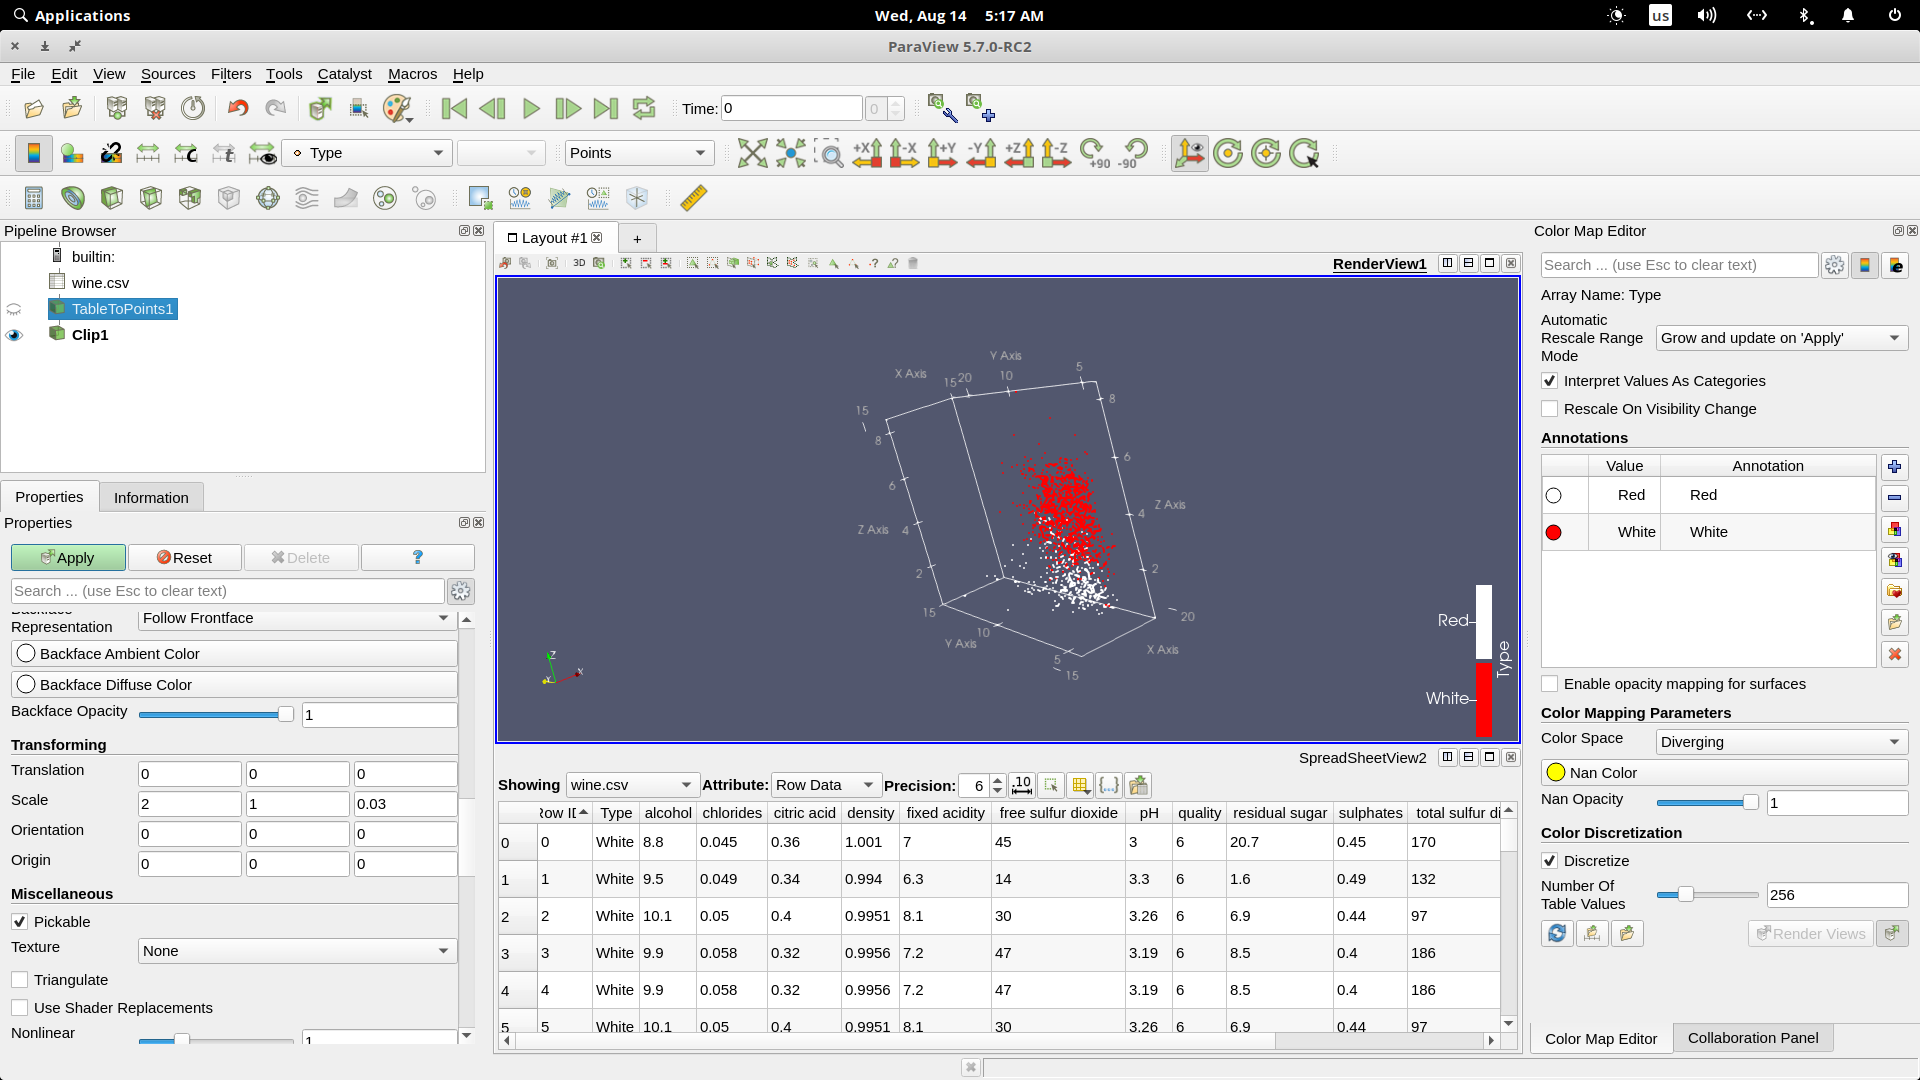
\includegraphics[scale=0.2]{paraview}
\caption{Result of our example workflow.}
\label{fig:paraview}
\end{figure}

Other key parts of the user interface include a properties panel, which allows the user to modify parameters of a selected action in the pipeline, and the work area where visualizations are drawn. The user is also able to display other panels, which contain further statistical information on loaded dataset. Of particular note is the \emph{Color Map} panel, which enables the user to choose between various color spaces. 

There is also a \emph{Collaboration} panel, which enables multiple users to connect to one another using a local-area network and share the current state of the work area as well as communicate with one another using text messages. The user roles are clearly defined --- one user acts as a master and has the ability to edit the project, while others act as slaves and cannot interact with the visualization.

We will start our usability test by opening our CSV file. ParaView supports a countless amount of input formats. After loading the data, it is analyzed and data types are automatically assigned, the user can choose a delimiter character and specify whether the dataset in question includes headers. To finish the loading process, the user has to click on the \emph{Apply} button. After loading the dataset they are presented with a tabular view of it in its entirety.

\begin{figure}[ht]
\centering
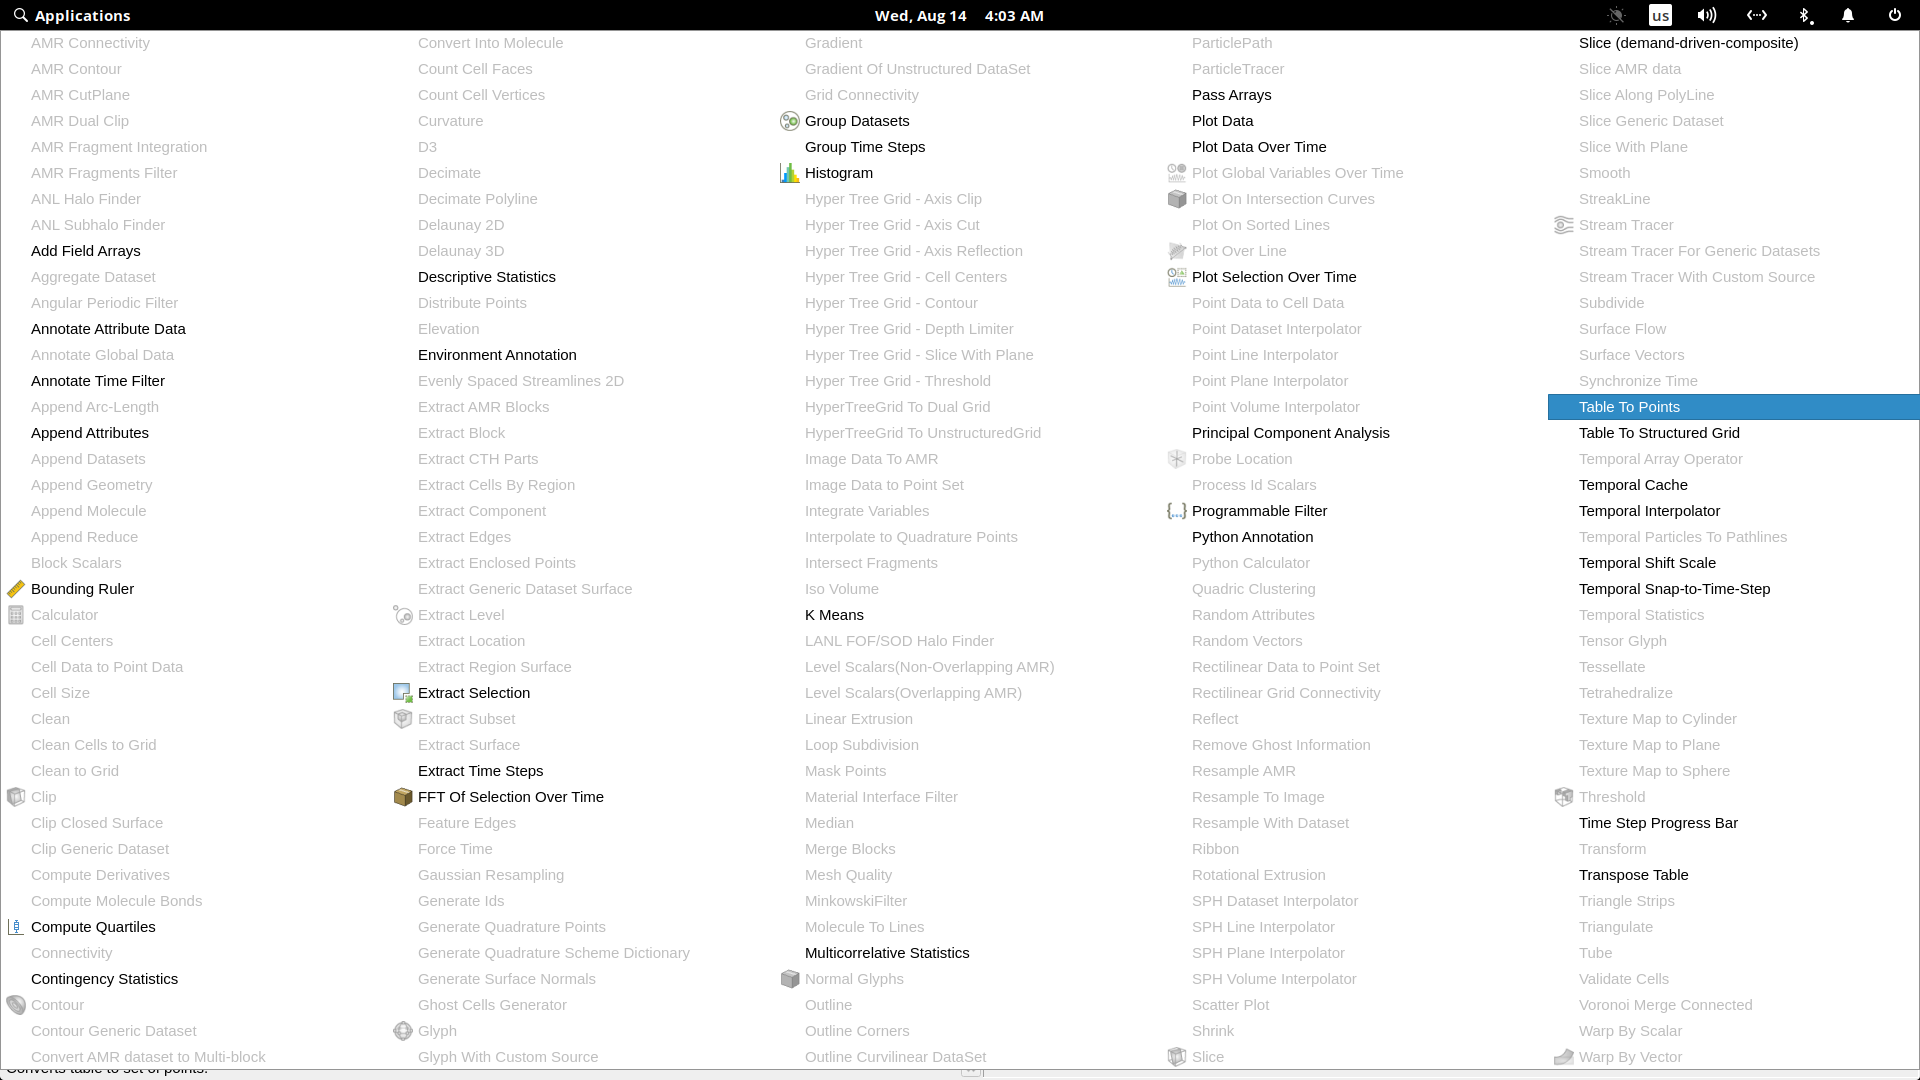
\includegraphics[scale=0.2]{paraview_menu}
\caption{Menu listing all available filters.}
\label{fig:paraview_menu}
\end{figure}

Next, we need to create a scatter plot. This is done in a very convoluted fashion by first selecting the dataset action in the pipeline browser and then opening up a menu via \emph{Filters \textrightarrow{} Alphabetical}. This menu takes up the entirety of the screen and contains many seemingly unrelated actions. An obvious choice for the user would be to select the \emph{Plot Data} option, however they must instead select \emph{Table to Points}.

The user is then free to select assignments for spatial axes using a drop down menu and map an attribute onto color in the same fashion. Clicking on \emph{Apply} and afterwards clicking on the eye icon next to the filter renders the plot.

The plot appears to be stretched, so we have to scale it by first pressing the cog icon to enable advanced options, and then modifying scale values for each axis in the \emph{Transforming} section by typing in random values until we are satisfied with the look of our plot.

As points are very small when we zoom in on the plot, we set \emph{Point Size} to a larger number. In order to be able to rotate the plot, we need to reset the pivot by pressing the \emph{Zoom To Data} button in ParaView's toolbar.

The next step is to slice the data by using the clip filter. We add the filter using \emph{Filters \textrightarrow{} Alphabetical \textrightarrow{} Clip}. It is appended to the end of our pipeline, however we need to copy the transform values to the new filter. Finally, we select the desired cutting plane using \emph{X/Y/Z Normal} buttons and drag the plane to a position that we would like. In order to view original axes, we select the result of \emph{Table to Points} filter in our pipeline.

The following table lists all KLM operations necessary to complete our task. The total time necessary to complete our tasks is 75.74 seconds. Overall, ParaView seems like a powerful tool, albeit with a very convoluted user interface. The tool's tutorial guide contains 159 pages, although it covers advanced functionality in its later chapters.

\begin{table}[]
\centering
\caption{Listing of KLM operations for ParaView.}
\label{klm-paraview}
\scalebox{0.7}{
\begin{tabular}{lll}
Operator & Description & Time (s)\\
M & Initiate opening a file & 1.35\\
M & Find file open button & 1.35\\
PB & Point at the button and press it & 1.3\\
PB & Select file and double click it & 1.3\\
M & Find properties panel & 1.35\\
PB & Point on \emph{Apply} button and press it & 1.3\\
M & Initiate plot addition & 1.35\\
PBPPB & Open up \emph{Filters} menu, navigate to \emph{Alphabetical \textrightarrow{} Table to Points} & 3.7\\
M & Find \emph{Properties} section of \emph{Properties} panel & 1.35\\
3*(PBPB) & Select assignments from dropdown & 7.8\\
M & Find \emph{Coloring} section of \emph{Properties} panel & 1.35\\
PBPB & Select an assignment from dropdown & 2.6\\
M & Find \emph{Styling} section of \emph{Properties} panel & 1.35\\
PBHKH & Change value of point size & 2.38\\
PB & Click on the eye icon to display filter & 1.3\\
M & Find \emph{Transforming} section of \emph{Properties} panel & 1.35\\
6*(PBHKKKH) & Guess transform scales that make length of plot's axes equal & 17.64\\
MPB & Find \emph{Zoom to Data} button and press it & 1.3\\
PBPPB & \emph{Filters \textrightarrow{} Alphabetical \textrightarrow{} Clip} & 3.7\\
PBPB & Click on the eye icon next to the two recently added filters & 2.6\\
M & Find \emph{Transforming} section of \emph{Properties} panel & 1.35\\
3x(PBHKKKH) & Fill in scale values from the previous filter & 8.82\\
M & Find \emph{Plane parameters} section of \emph{Properties} panel & 1.35\\
PB & Point and click on desired normal button to create a cutting plane & 1.3\\
PBPB & Drag the cutting plane to desired position & 2.6\\
PB & Click on \emph{Apply} & 1.3\\
PB & Select original filter to display its axes & 1.3
\end{tabular}
}
\end{table}


\subsection{Tableau}

Tableau is a commonly used software for business intelligence. It allows the user to load data by opening a local file (CSV, JSON, Excel spreadsheet) or connecting to a database (MSSQL, Oracle, MySQL, Amazon Redshift and more). The number of database integrations is much larger than the number of supported types of local files indicative of the product's focus on enterprises and big data. The desktop application is available for Windows and macOS.\autocite{tableau} The company also offers a product called Tableau Server which enables the users to store their data online using either a publicly hosted service or an on-premises server.

The client software includes a very straightforward and easy-to-use interface. The user loads a dataset and is presented with a tabular view. Data types are automatically detected, as is the column delimiter (in the case of CSV files). In this view, the user is also able to pre-filter data by selecting a threshold and filling in null values. They are then able to create a \emph{sheet}, a metaphor commonly used in spreadsheet software. The user then selects attributes they would like to use by dragging them into a \emph{Dimensions} list and afterwards can map them onto rows, columns and non-spatial features of the two-dimensional scatter plot.

Unfortunately, as of version 2019.2.2, Tableau does not have native support for three-dimensional plots. There is a workaround for creating pseudo-3D plots, but it requires the use of a SQL database and is not user-friendly at all, being more of a hack than a proper solution.\autocite{tableau3d}

The following table lists all KLM operations necessary to complete a simplified task of creating a two-dimensional scatter plot.

\begin{table}[]
\centering
\caption{Listing of KLM operations for Tableau.}
\label{klm-tableau}
\scalebox{0.7}{
\begin{tabular}{lll}
Operator & Description & Time (s)\\
M & Initiate opening a file & 1.35\\
M & Find \emph{More...} button on sidebar & 1.35\\
PB & Point at the button and press it & 1.3\\
PB & Select file and double click it & 1.3\\
M	& Locate \emph{Sheet1} tab & 1.35\\
PB & Point at the tab and press it & 1.3\\
M & Locate \emph{Measures} and \emph{Dimensions} lists & 1.35\\
3*(PBPB) & Move attributes we want to display from \emph{Measures} to \emph{Dimensions} & 7.8\\
M & Locate plot dimension settings & 1.35\\
2*(PBPB) & Move spatial attributes from \emph{Dimensions} list to \emph{Columns} and \emph{Plots} respectively & 5.2\\
2*(PBPB) & Click on both assignments and select \emph{Continuous} from dropdown menu & 5.2\\
PBPB & Move one attribute from \emph{Dimensions} onto \emph{Color} subsection of \emph{Marks} panel & 2.6\\
M & Locate the axis we want to slice & 1.35\\
PBPB & Right click on the axis and select \emph{Edit Axis} from dropdown & 2.6\\
PB & Select \emph{Fixed} radio button & 1.3\\
PBHKKKH & Input desired value to \emph{Fixed end} textbox & 2.94\\
PB & Close the modal & 1.3
\end{tabular}
}
\end{table}

The total time necessary to complete our tasks is 40.94 seconds, half the time of a similar workflow in ParaView. However, we have only been able to create a two-dimensional scatter plot due to software's limitations.

\begin{figure}[ht]
\centering
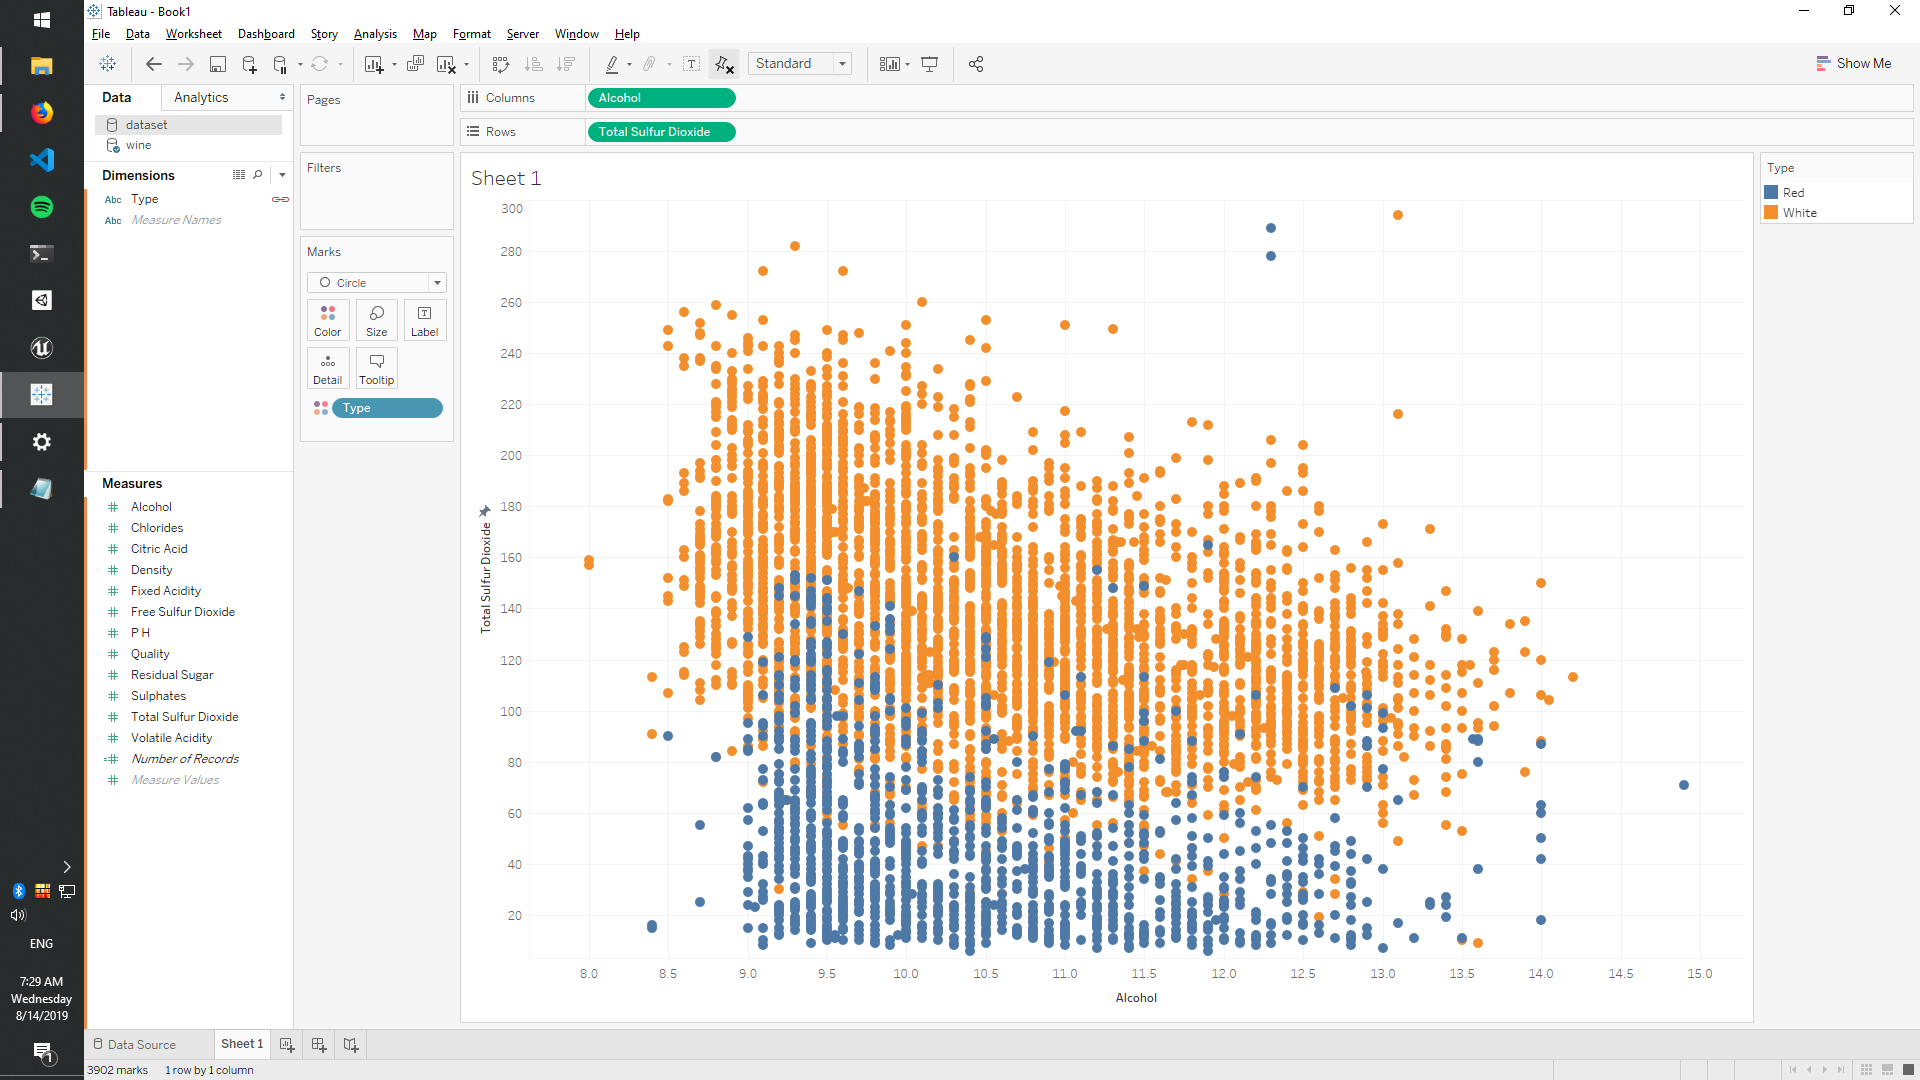
\includegraphics[scale=0.2]{tableau_sheet}
\caption{Tableau's sheet view.}
\label{fig:tableau_sheet}
\end{figure}

\begin{figure}[ht]
\centering
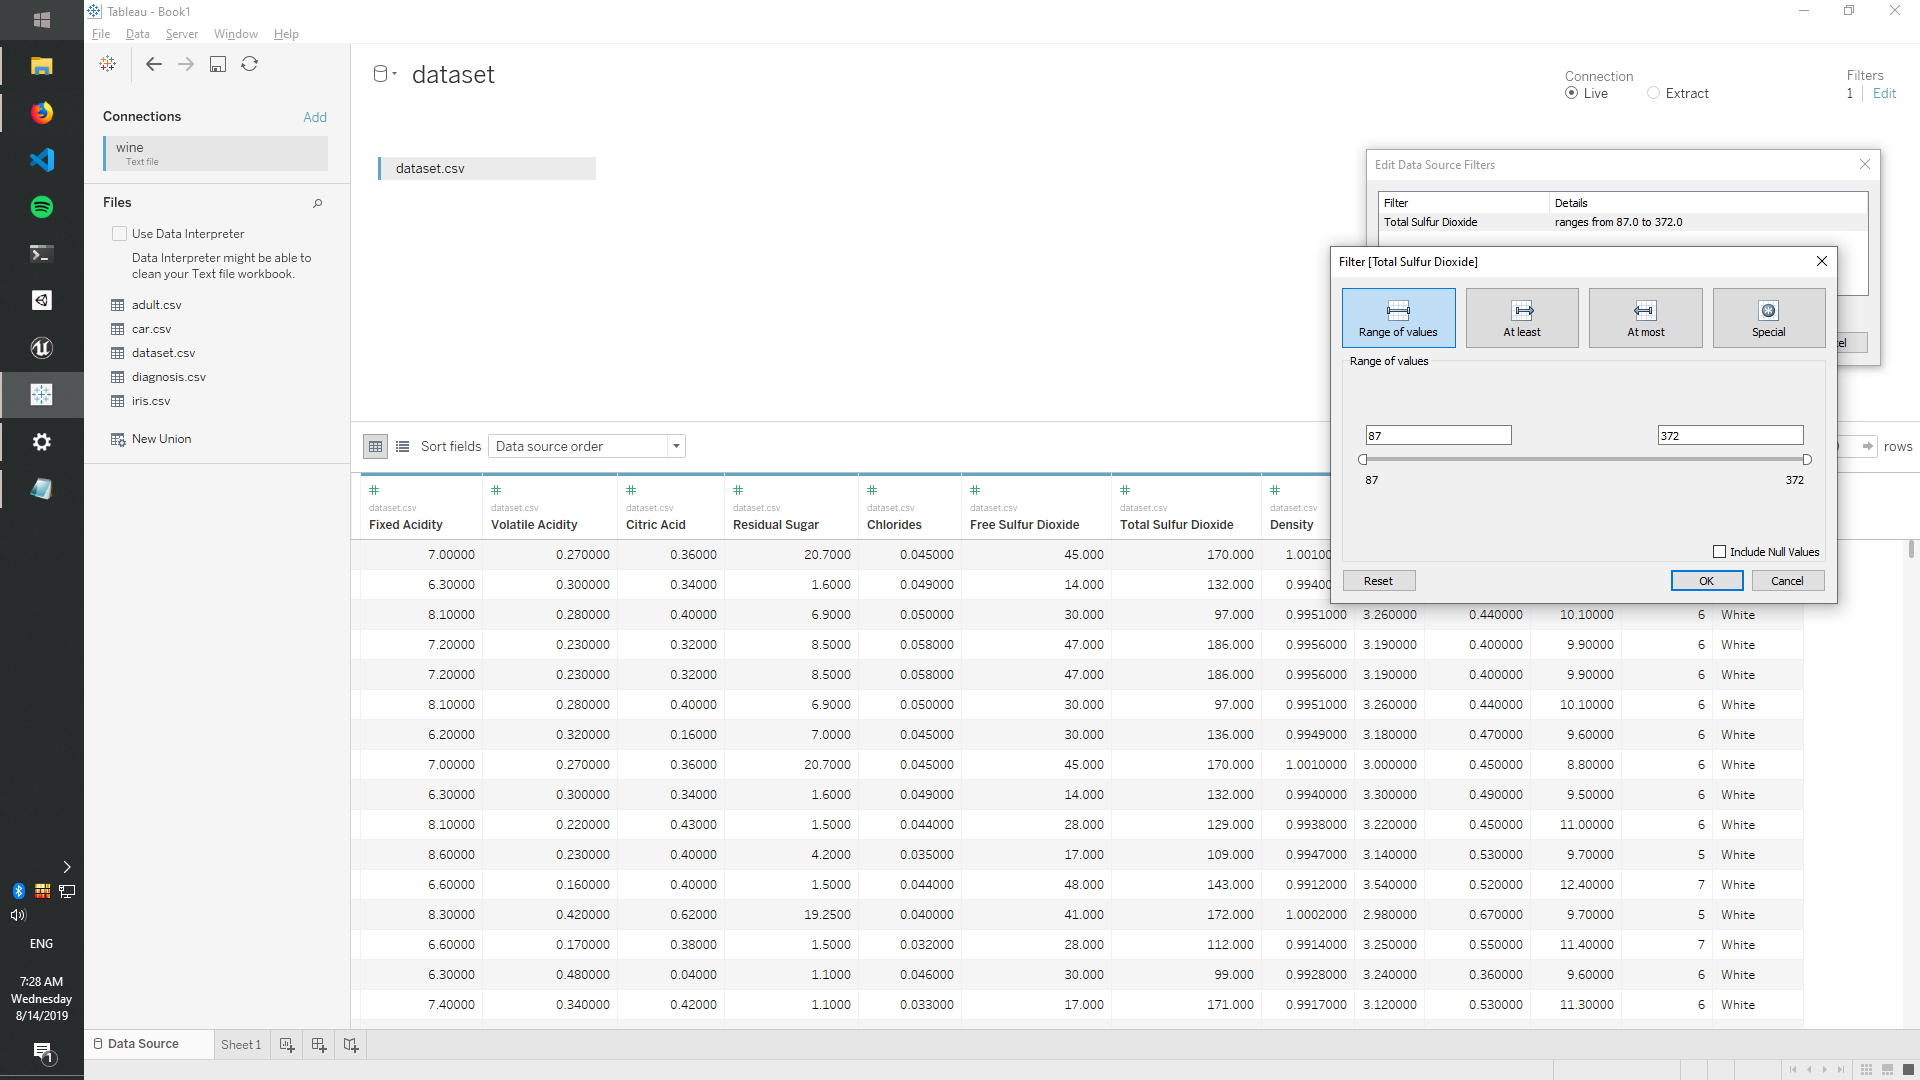
\includegraphics[scale=0.2]{tableau_edit}
\caption{Tableau's edit view.}
\label{fig:tableau_edit}
\end{figure}

\newpage

\section{Benefits of virtual reality}

We believe that virtual reality has the potential to enhance the visualization experience. Let us explore several reasons why.

\subsection{Stereoscopic view, 6DOF}

Head-mounted displays (HMD) are by design stereoscopic. One study compared error rates of visualization analysis on a conventional monitor against a stereoscopic solution with eye separation (interpupillary distance, IPD) of 6.4 cm. It also focused on the benefits of dynamic motion for perception.

The findings were that the use of both dynamic motion and stereoscopy significantly reduced error rates (by 10\% in inexperienced participants, n=14 and 15-30\% in experienced participants, n=2). Combination of these two methods led to further improvement.\autocite{ware}

With modern HMDs we can leverage both of these methods as 6 degrees of freedom (6DOF) headsets allow the user to freely position their head in space, simulating motion.

\subsection{Spatial interface}

Researchers and designers alike have been looking at replacing the traditional Windows-Icons-Menus-Pointing (WIMP) desktop metaphors with 3D alternatives since the early 90s. The new interfaces instead rely on hand gestures and speech recognition to navigate around 3D space. One article from the era argues that users are frustrated by many layers of \emph{point and click} and visual clutter that is common with WIMP UIs and discusses the limitations of relying exclusively on the sense of sight. The author prophesizes rise of virtual reality and proceeds to discuss potential applications.\autocite{wimp}

Innovative examples such as Google Earth VR prove that well-designed spatial interfaces have the potential to make UI more intuitive, especially to first-time users.\autocite{earthux}

\newpage

\subsection{Immersive analytics}

The full use of one's visual field as well as senses of touch (through force feedback) and spatial sound allow the user to fully immerse themselves into their data, which has potential to improve their concentration. Furthermore, they have the ability to invite other users into their virtual space, which allows for multi-user interactions with plots inside the space.

\chapter{Domain analysis}

In this chapter, we will analyze the state of virtual reality in 2019 and take a look at a couple examples of applications in the space of immersive analytics. Furthermore, we will define our target group and set design goals to help narrow down our scope.

\section{Target group}

Our application should provide an intuitive way to view data in a virtual reality environment in an attempt to leverage the spatial properties and immersion. It should be friendly enough to be accessible to users with basic computer skills while also providing advanced functionality to power users via API integrations.

\section{Target platform}

In order to specify a baseline for our application, we first need to look at the current landscape of virtual reality hardware. Over the years, we have primarily been dividing virtual reality systems into two main categories --- phone- and PC-based VR. The former category includes ecosystems like Google Cardboard\autocite{cardboard}, Daydream\autocite{daydream} and Samsung's GearVR\autocite{gearvr}, while the latter includes three primary vendors --- Oculus with its Rift headset\autocite{rift}, Microsoft's Windows Mixed Reality\autocite{wmr} ecosystem composed of head-mounted displays (HMDs) made by third-party manufacturers and Valve's SteamVR\autocite{steamvr}, which includes support for pretty much any PC-based headset.

\begin{figure}[ht]
\centering
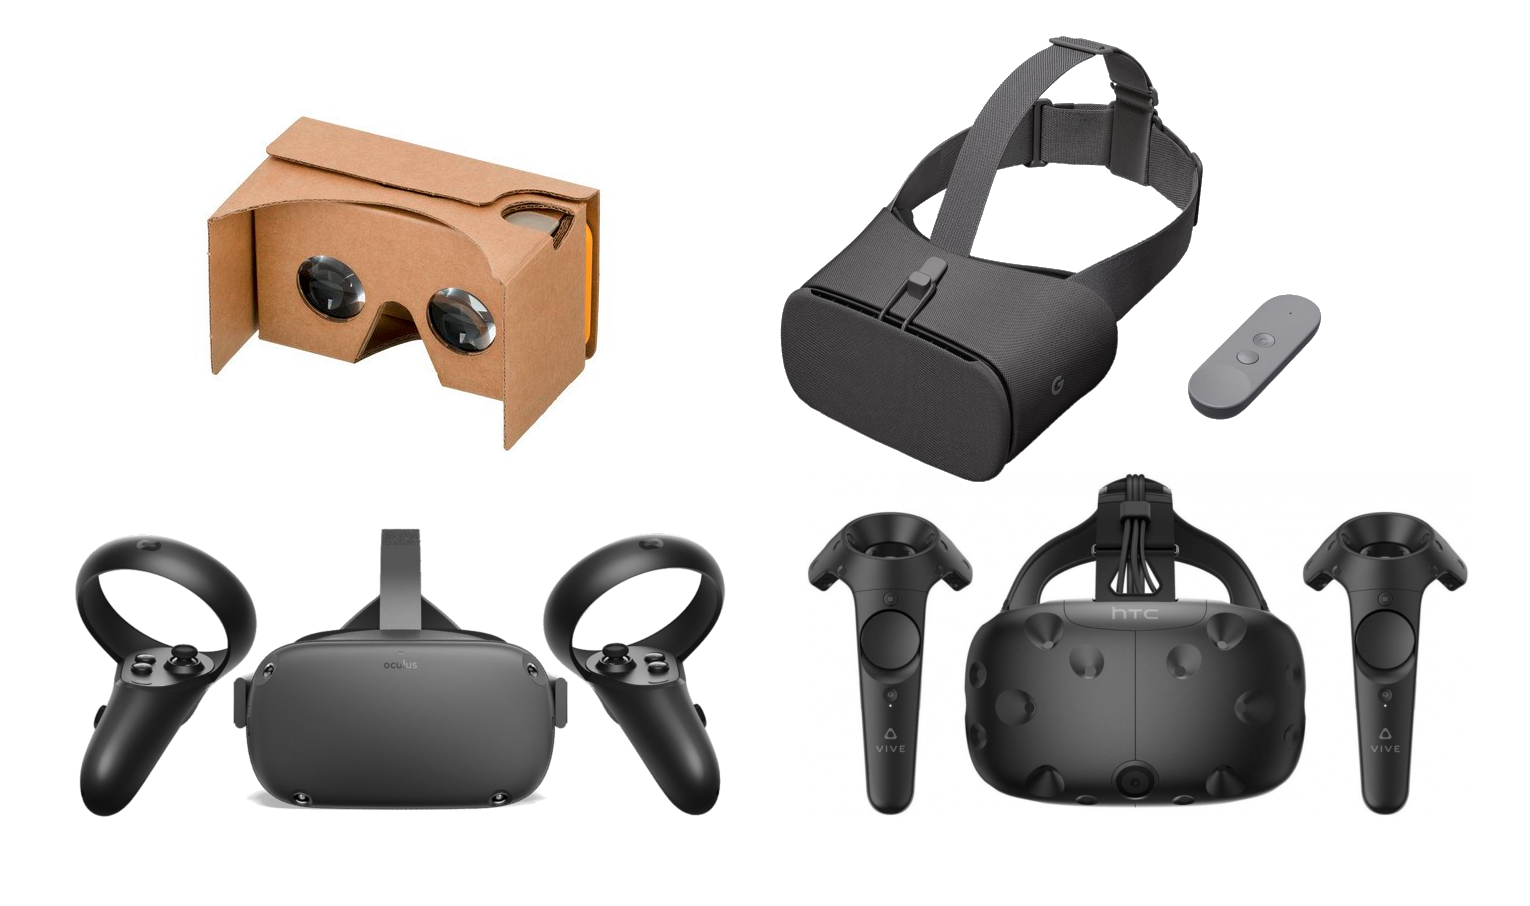
\includegraphics[scale=0.2]{hmd_examples}
\caption{Examples of various contemporary virtual reality systems. Clockwise from top: Google Daydream View (mobile), HTC Vive (PC), Oculus Quest (standalone), Google Cardboard (mobile).}
\label{fig:hmd_examples}
\end{figure}

There are two primary differences between the two mentioned categories. The first concerns system resources available to developer. Graphics processing units (GPUs) in modern personal computers are significantly more powerful than their handheld counterparts and as such, the software can be ran at much higher fidelity. To get a rough idea on performance targets for PC and mobile, we can consult Oculus's development documentation. The recommended limit for draw calls and vertices is 100 and 100,000 for mobile and 1,000 and 2,000,000 for PC, more than a ten-fold difference.\autocite{oculusperftargets} We also have to keep in mind that this number is based on minimum requirements for Oculus Rift headset, which mention an Nvidia GeForce GTX 1050 Ti, a relatively low-spec GPU.\autocite{riftspecs}

The second difference has to do with capabilities in regards to sensing movement and rotation of controllers and the HMD itself. Mobile headsets are limited to 3 degrees of freedom (DOF), making use of rotational data from the phone's inertial measurement unit (IMU), whereas PC-based systems generally offer 6 degrees of freedom (6DOF), which enables developers to utilize position as well as rotation. Controllers typically offer an array of buttons, digital/analog triggers and either a thumbstick or touchpad. The most basic VR systems do not offer a controller at all (Google Cardboard) or a non-tracked controller (also referred to as 0DOF; early iterations of Oculus Rift). These systems are restricted to gaze-based interaction techniques such as \emph{dwell selection}, where an action is triggered by lining up a reticle at the center of the screen with an object and keeping the head still for a defined period of time.\autocite{bookofvr}

\begin{figure}[ht]
\centering
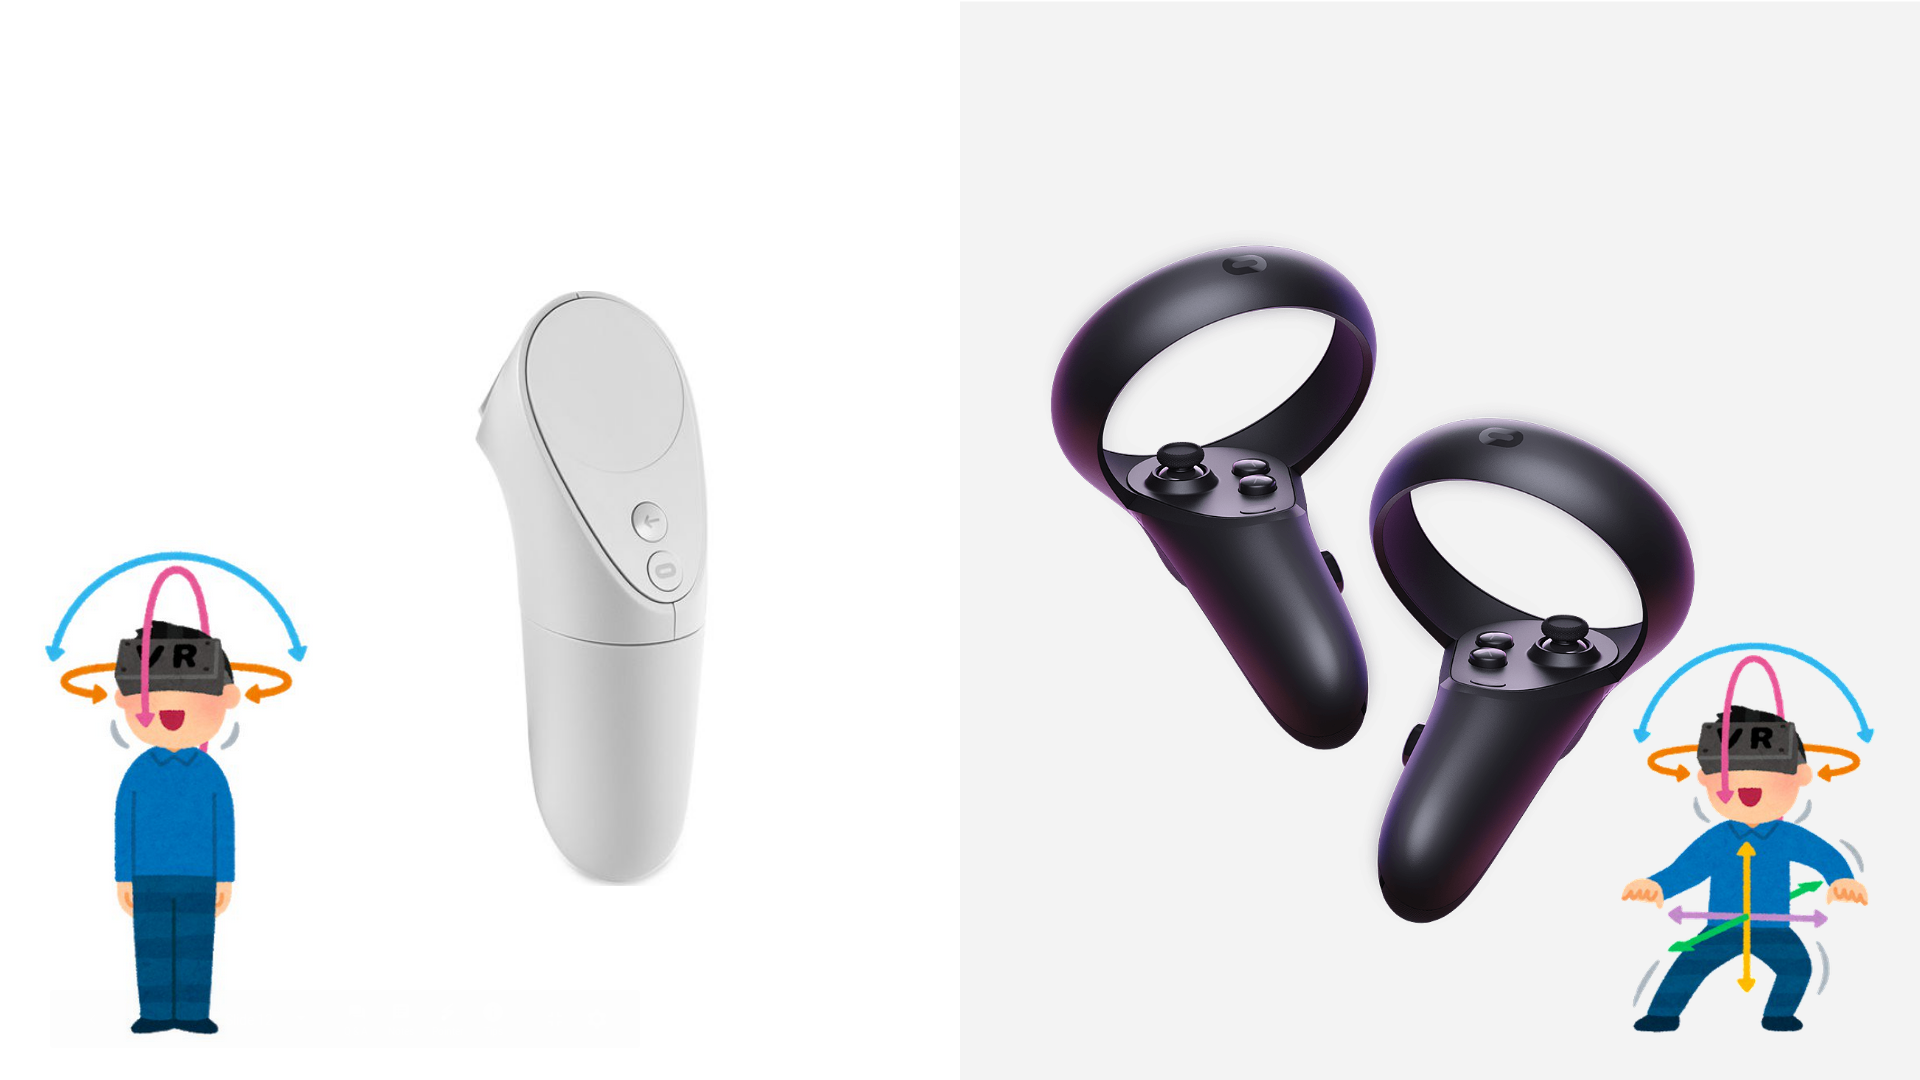
\includegraphics[scale=0.2]{dof_explanation}
\caption{Left: Oculus Go controller offering 3 degrees of freedom. Right: Oculus Touch 6DOF controller.\autocite{dofexplanation}}
\label{fig:dof_explanation}
\end{figure}

The last two years saw a shift from phone-based VR into a completely new category of standalone virtual reality hardware, composed of headsets like Oculus Quest\autocite{quest}, Oculus Go\autocite{go} and HTC Vive Focus\autocite{vivefocus}. These headsets offer a much better end-user experience and reduce barrier to entry by removing the need for a powerful computer or a compatible smartphone. Technical capabilities of these devices are somewhere in between the two traditional categories with devices like Oculus Quest offering 6DOF inside-out tracking capabilities and ability to run graphically optimized versions of content previously exclusive to PCs.

In order to start designing our application, we first have to decide on baseline hardware as all future design decisions have to take into consideration technical limitations of targeted devices. In order to support the largest possible user base, we aim to support all classes of VR systems. To keep development manageable, we will primarily target Oculus hardware. We have chosen this particular company as it encompasses all three categories (PC, mobile, standalone) with its devices. The only ecosystems we will not support are Google Cardboard due to lack of hand controllers (and thus the necessity of designing around gaze-based interaction methods) and Google Daydream due to the recent discontinuation of the platform.\autocite{daydreameol}

\section{State of the art}

In this part we will focus on analyzing existing VR-enabled visualization tools. Emphasis is given on select features that author perceives as relevant. We will explore data support to see how we can load data onto the platform, as well as options for extensibility via plugins. Due to the rise of mobile HMDs, we will look at how well they are supported in each product. From the feature set, we will focus on machine learning capabilities and collaboration features. Lastly, we will take a quick look at business models of companies that develop these applications and check availability of editions aimed at end consumers and/or academia.

\subsection{Virtualitics}

Virtualitics aims to combine the benefits of high-dimensional visualization in VR with those of AI-driven data analysis.\autocite{virtualitics} It includes a Windows application for loading, editing and visualizing data in both desktop mode and VR, the latter enables the user to visualize data in an immersive environment as well as to collaborate with other users who are represented by avatars. Virtualitics also offers a Python API, which enables programmers to implement an integration into their applications. This API is available in the Python repository under a FOSS license (MIT).\autocite{pyvip}

\begin{figure}[ht]
\centering
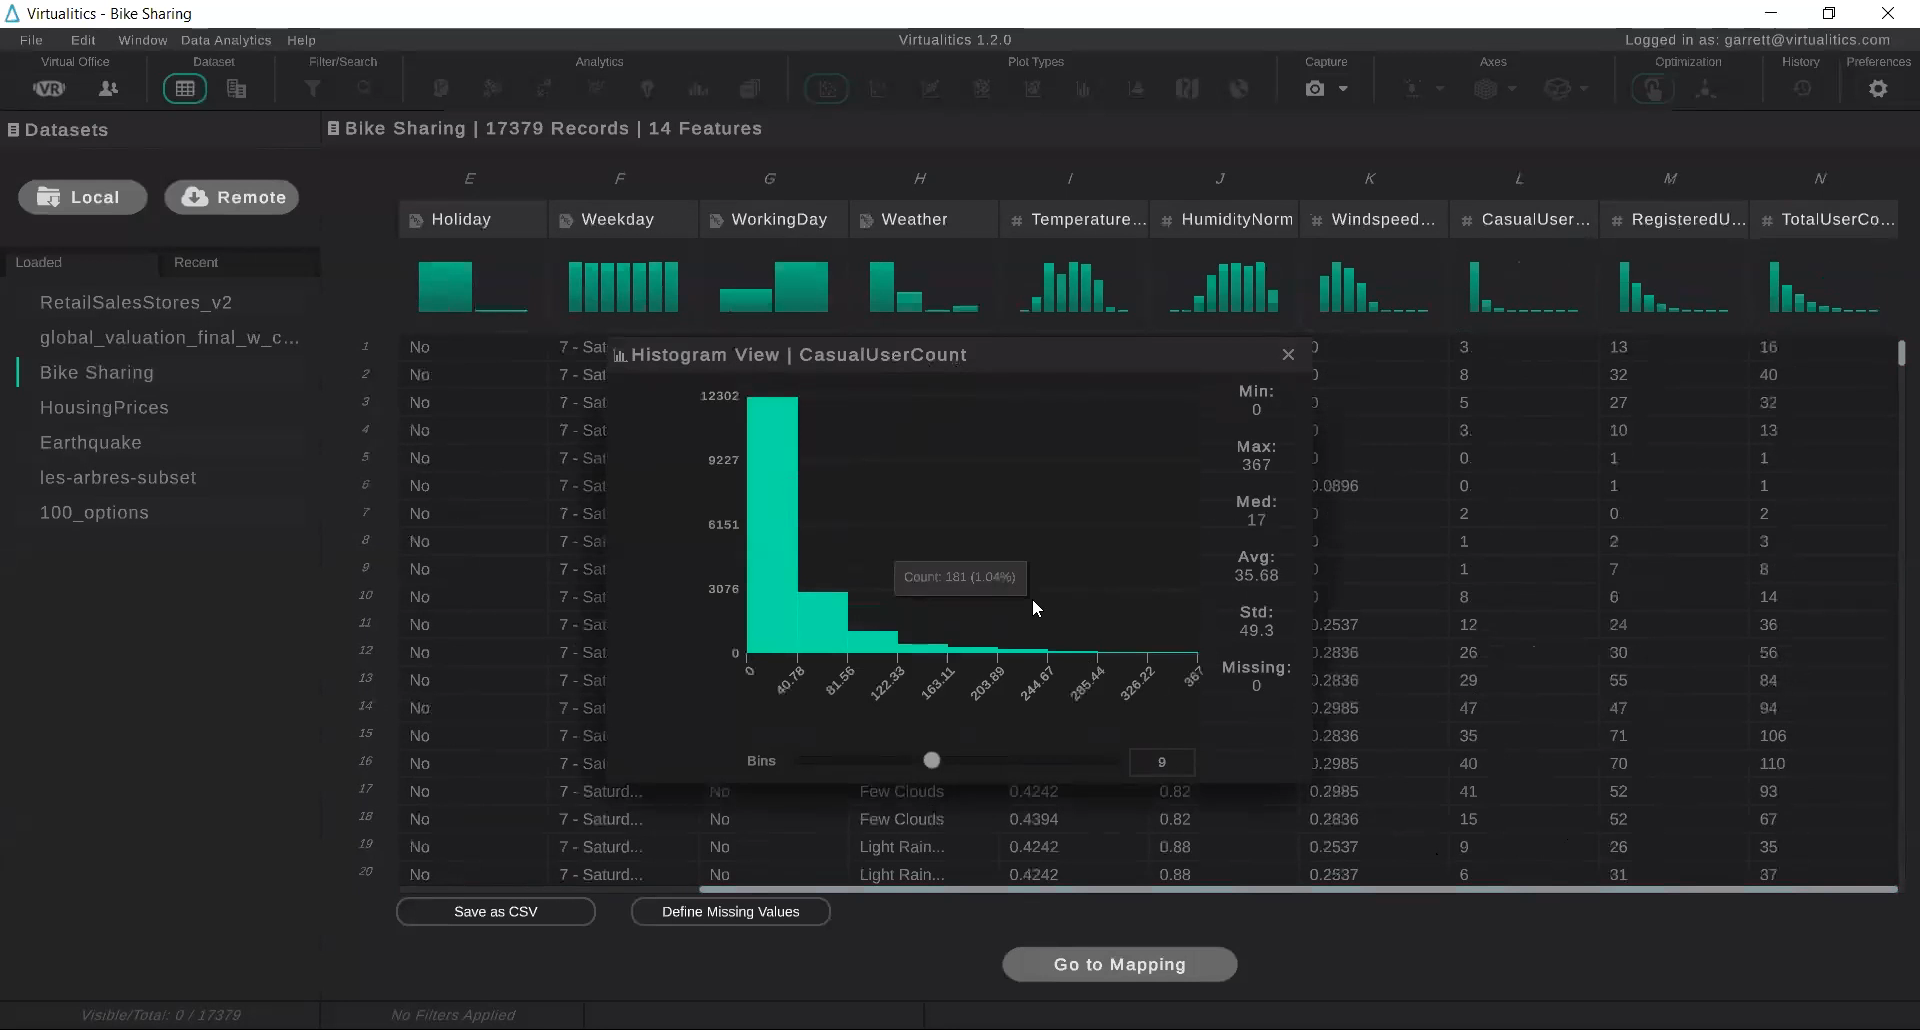
\includegraphics[scale=0.2]{virtualitics_spreadsheet}
\caption{Spreadsheet view in Virtualitics's desktop application.\autocite{virtualiticsvideo}}
\label{fig:virtualitics_spreadsheet}
\end{figure}

The interface of Virtualitics's desktop application bears resemblance to Tableau. Data can be loaded from either a local file or a remote database. It includes a \emph{spreadsheet view}, which shows loaded data in a tabular form with histograms and basic statistical information such as mean and median. The user is able to filter data and fill in missing values.

\newpage

Afterwards, they are able to switch into the \emph{mapping view}, which allows them to map attributes onto dimensions. A unique feature called \emph{smart mapping} offers the user a selection of attributes that are calculated to be the most important in the dataset. The user can also toggle between multiple plot types.

\begin{figure}[ht]
\centering
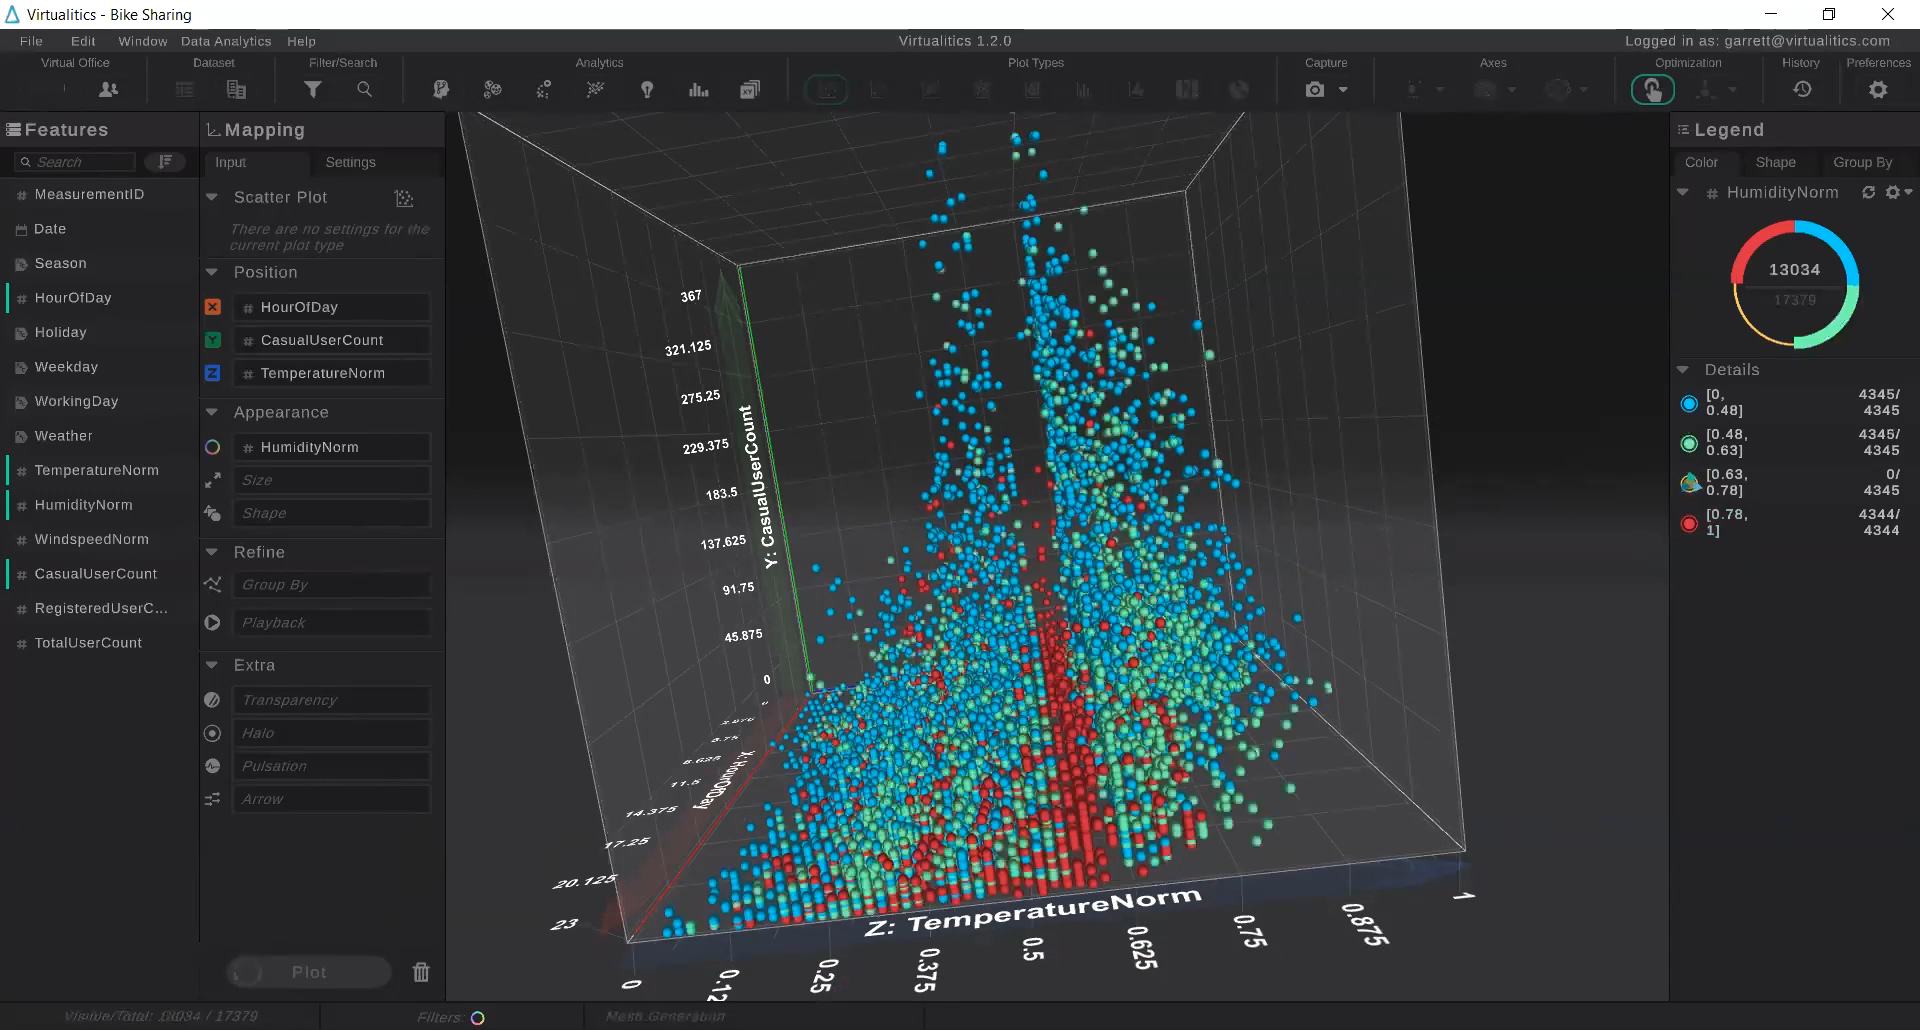
\includegraphics[scale=0.2]{virtualitics_mapping}
\caption{Mapping view in Virtualitics's desktop application.\autocite{virtualiticsvideo}}
\label{fig:virtualitics_mapping}
\end{figure}

The VR component dubbed \emph{Virtual Office} allows the user to interact with plots they have defined in the \emph{mapping view} in VR. They are able to access key features of the desktop application using flat panels which have the same appearance as in desktop mode. The user can interact with one 3D plot at a time, which is located at the center of the virtual space with 2D plots surrounding the user and offering more insight. The software includes a collaboration feature, enabling the user to invite other stakeholders into their virtual environment.

Virtualitics's Python API enables the user to connect to a running instance of the desktop application and load data from a Pandas data table as well as access certain analytics and visualization features straight from their code.

\begin{figure}[ht]
\centering
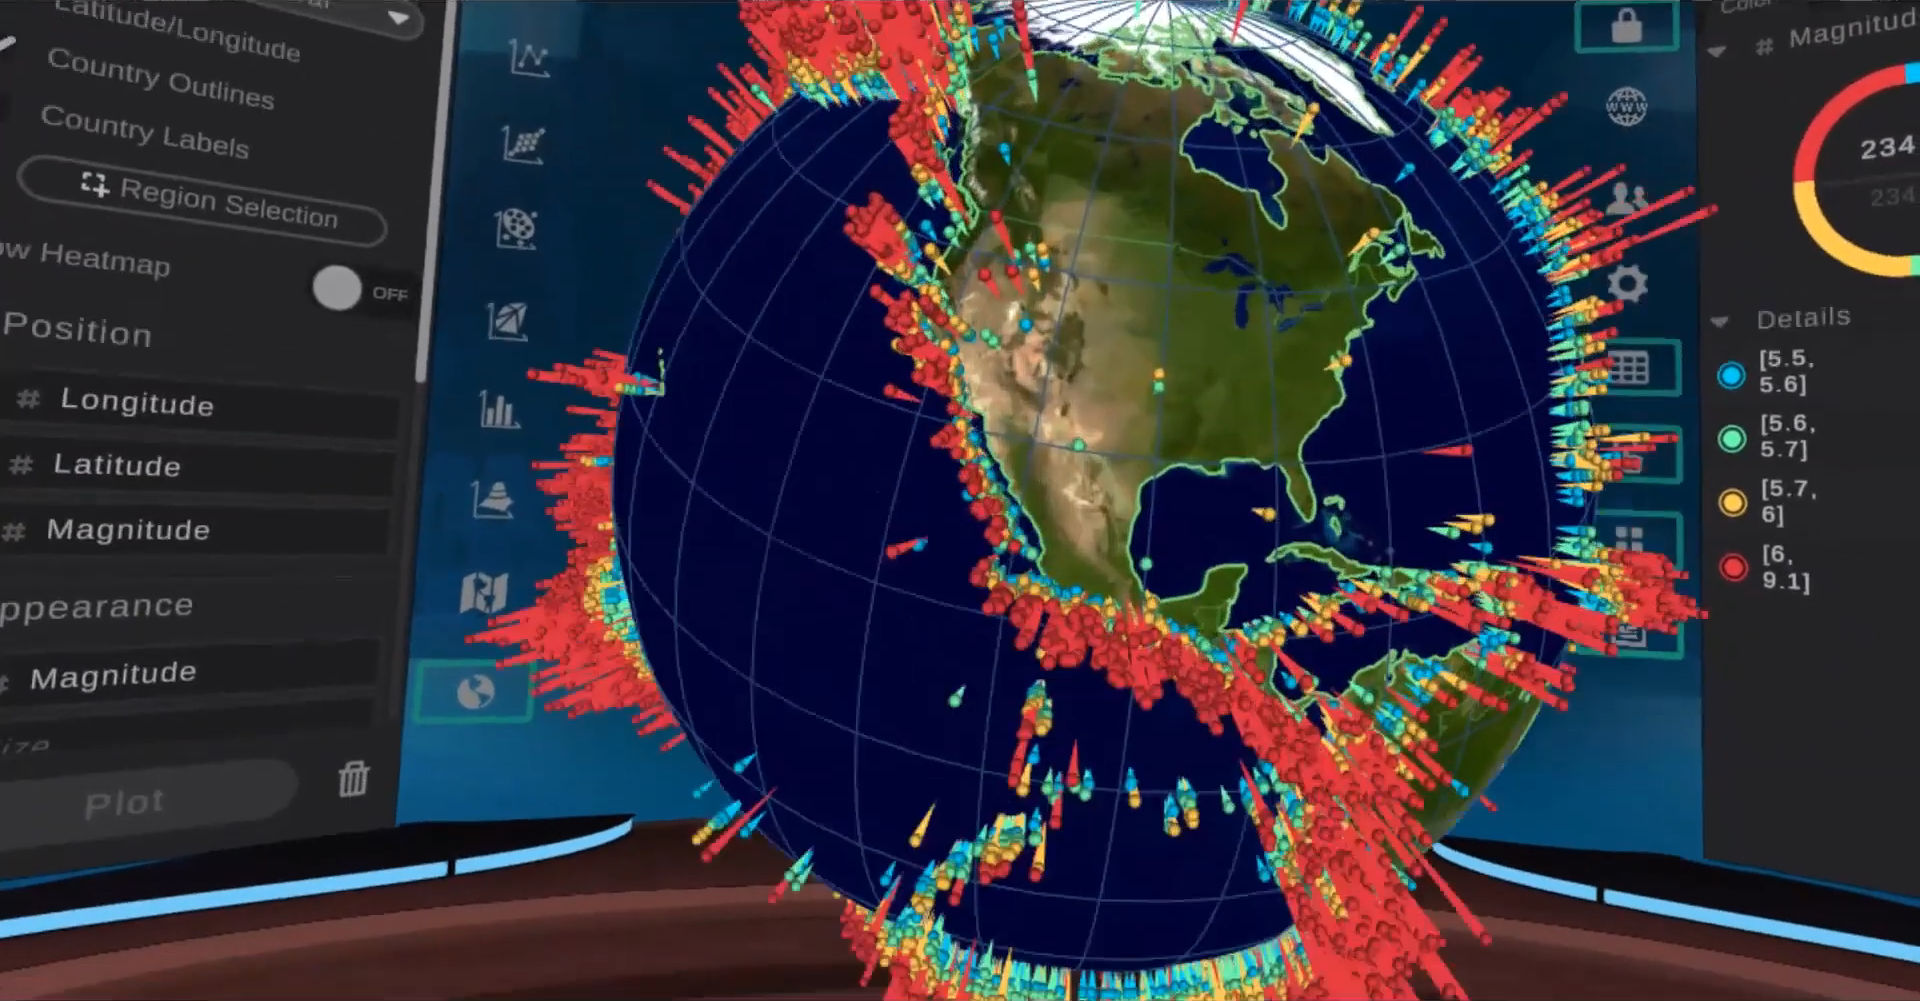
\includegraphics[scale=0.2]{virtualitics_vr}
\caption{Virtualitics's VR interface.\autocite{virtualiticsvideo}}
\label{fig:virtualitics_vr}
\end{figure}

Virtualitics includes support for Oculus Quest, however it is interesting to note that due to its limited hardware capabilities, arbitrary limits are in place for dataset size and number of points rendered in plots. If the point limit is reached, the software renders them as 2D billboards rather than as meshes.\autocite{virtualiticsquest}

Out of the three products that we have analyzed, Virtualitics seems to be the most advanced. It offers a very clean task-driven user interface, powerful tools for analytics, mobile support for Oculus Quest, large number of integrations with an open-source Python API and collaboration features. Negatives include proprietary nature of all other components, which requires users to resort to the aforementioned Python API, lack of support for 3DOF headsets such as Oculus Go or Google Daydream, VR interface that is perhaps too similar to its desktop counterpart and does not fully utilize the capabilities of room-scale VR and, as with all other products mentioned, lack of any consumer or academic version.

\subsection{LookVR}

LookVR is a virtual reality tool for exploring data that is part of Looker, an enterprise business analytics platform.\autocite{lookvr} Looker enables its customers to connect to more than 50 types of databases. Their BI platform can be accessed via a web browser, a demo of an example dashboard is available.\autocite{lookerdash} LookVR enables the user to access 3D scatter plots, bar plots as well as more unorthodox plot types hosted on Looker. There does not seem to be any interactivity at all outside of selecting a plot. The software allows the user to push a cartoon-like \emph{big data} button in order to enlarge the visualized plot.

\begin{figure}[ht]
\centering
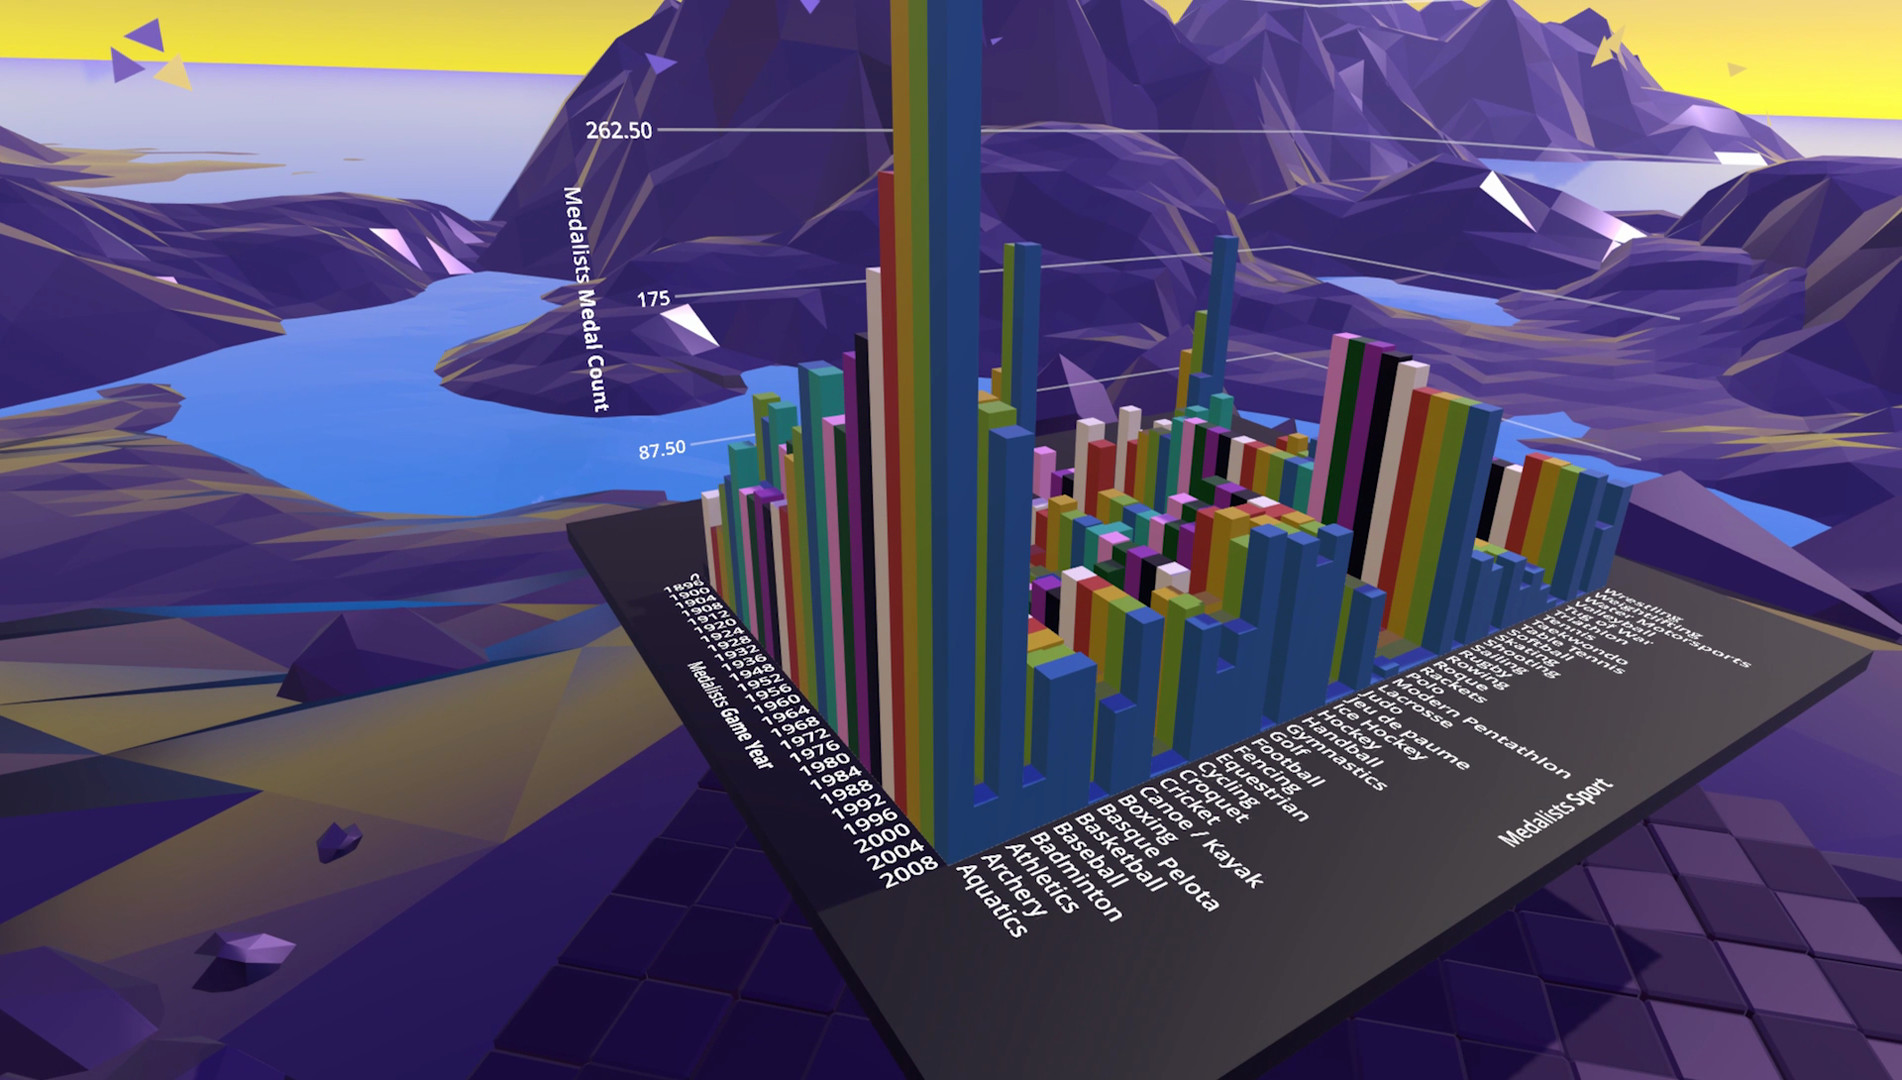
\includegraphics[scale=0.2]{lookvr}
\caption{LookVR's user interface.\autocite{lookvrsteam}}
\label{fig:lookvr}
\end{figure}

LookVR is available for free via Steam.\autocite{lookvrsteam} If the user's company has access to Looker, they may log in using their credentials, otherwise a small selection of plots is available as a sample. Unfortunately, all of our attempts to load sample data have ended unsuccessfully.

When it comes to LookVR's feature set, it is rather basic. The amount of available plot types is small, there is no support for mobile HMDs, no extensibility or FOSS components and although it is distributed for free via Steam, the requirement of a Looker license does not allow non-enterprise customers to utilize the product.

\subsection{3Data}

Austin-based startup 3Data started as a 2016 prototype called DataVizVR.\autocite{datavizvroculus} As of January 2020, this demo is still available via Oculus Store. The demo features a number of preloaded datasets and enables the user to interact with a single plot via a very spartan user interface. Since then, the product has matured, offering various plot types including terrain maps.\autocite{3data}

\begin{figure}[ht]
\centering
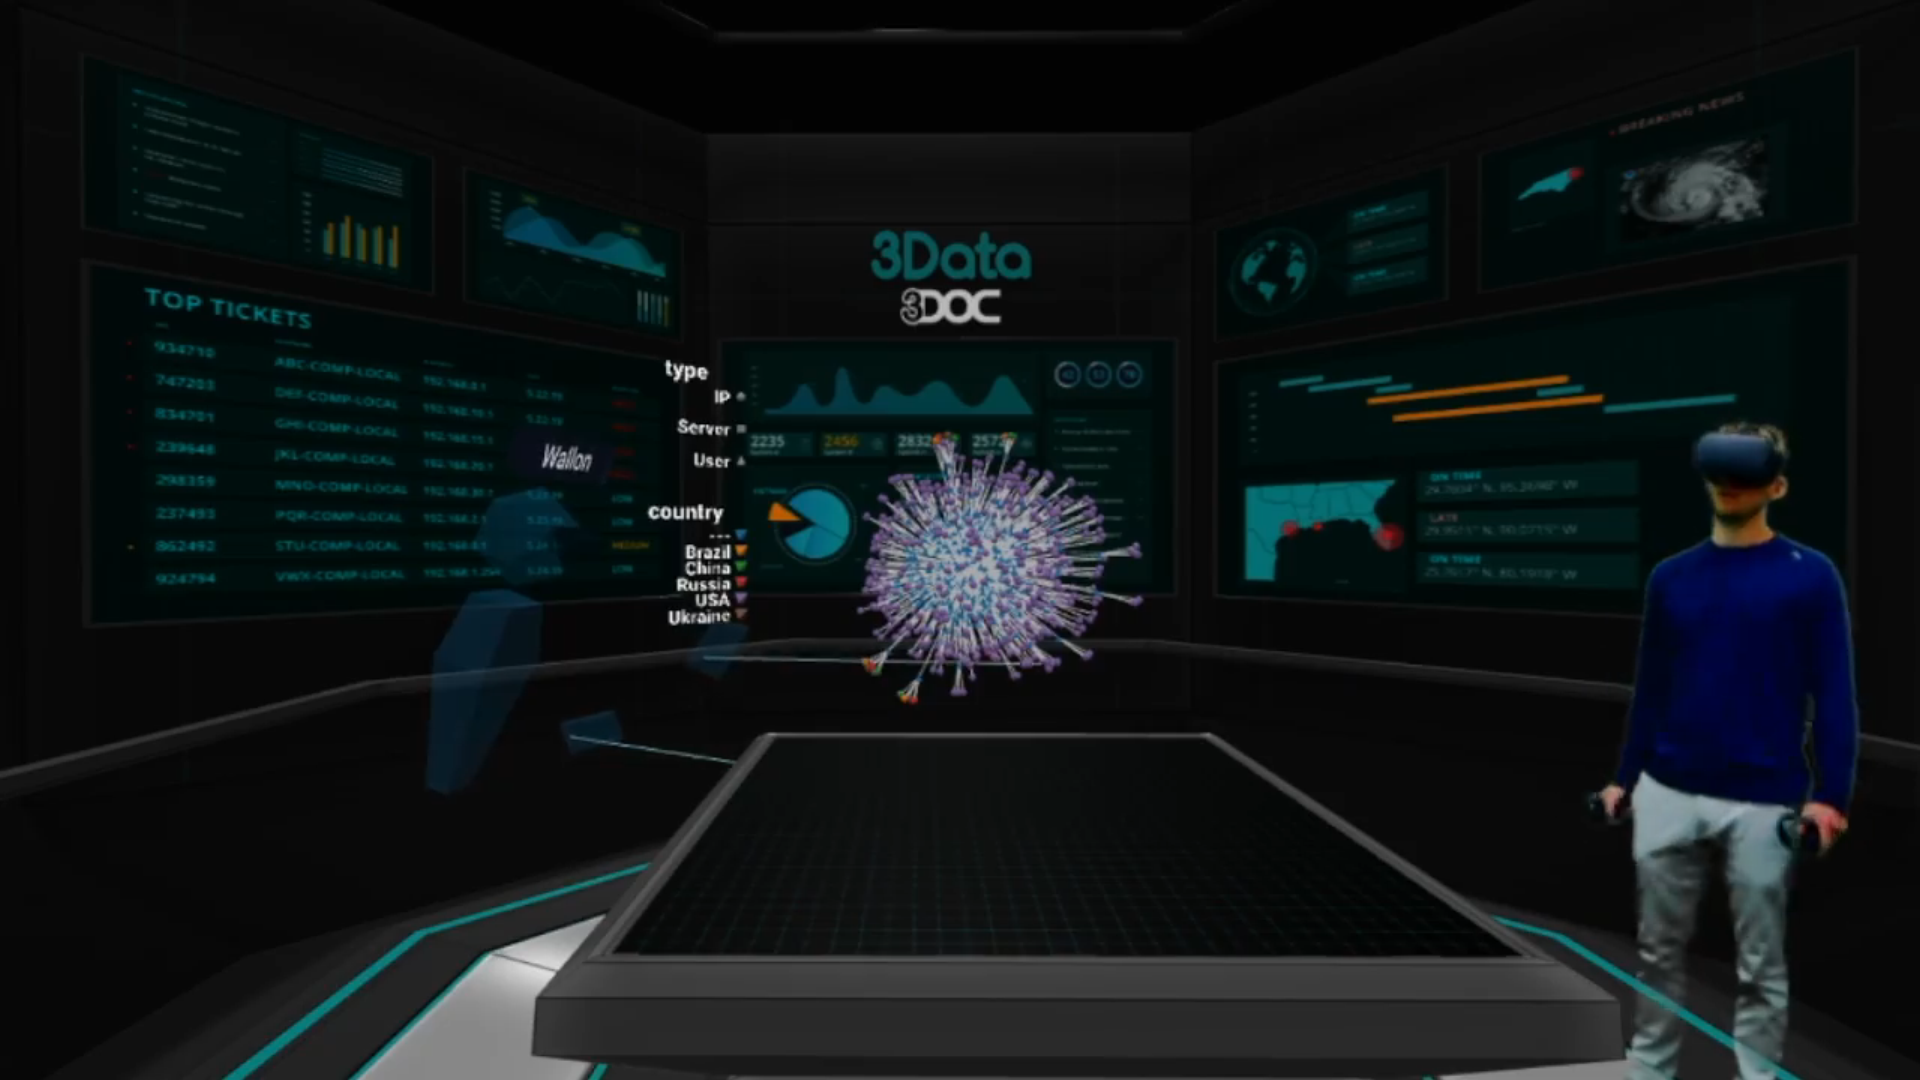
\includegraphics[scale=0.2]{3data}
\caption{3Data's immersive VR environment.\autocite{3datavideo}}
\label{fig:3data}
\end{figure}

Its user interface, dubbed \emph{3Data Operations Center}, seems similar to Virtualitics with a plot front and center and details surrounding the user in a virtual room, albeit slightly less polished. Like its competitor, 3Data also offers collaboration features.

\newpage

The product is sold solely to companies as an applications suite called \emph{3Data Power Office}, which in addition to the VR viewer includes tools for creating immersive presentations and collaboration with other stakeholders. Datasets can be self-hosted, 3Data promises direct connection to databases and existing BI tools.\autocite{3datasuite}

A defining feature of 3Data is its ability to run across multiple classes of devices. The visualization component is compliant with the WebVR specification, which enables it to run on VR/AR headsets, handheld mobile devices and personal computers in both 2D and immersive modes.\autocite{webvr} 3Data does not seem to offer a dataset editing tool of its own, relying instead on third-party applications.

At the moment, the product does not support any analytical features, however support for \emph{IBM Watson} is coming soon. After a detailed inspection, we concluded that there are no FOSS components whatsoever.

\subsection{Summary}

We have analyzed three products from the area of immersive analytics. The following chart compares their features.

\begin{figure}[!h]
\centering
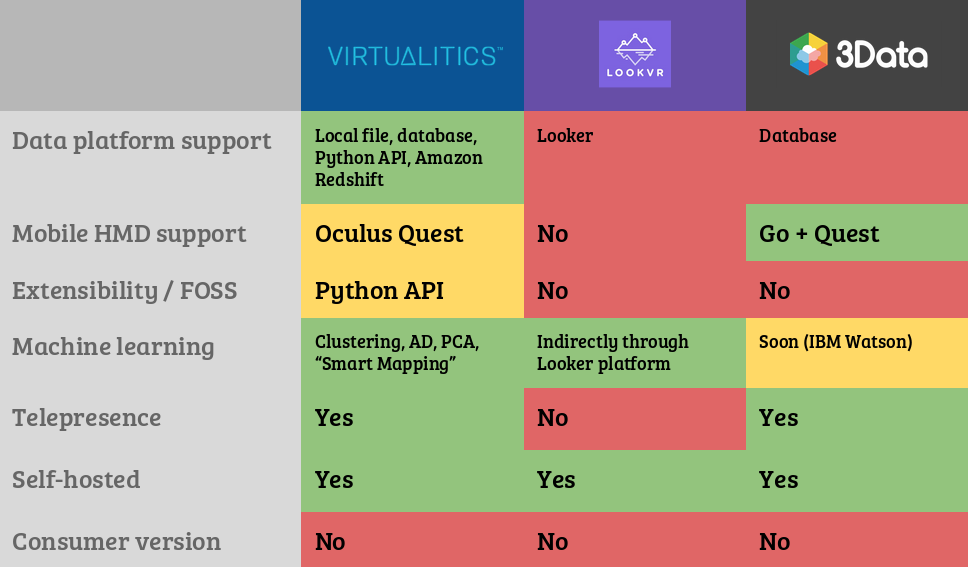
\includegraphics[scale=0.35]{comparison}
\caption{Comparison of VR data visualization applications.}
\label{fig:comparison}
\end{figure}

\chapter{Design}

In this chapter we will discuss in detail the target user group and use cases of our application, specify important goals that we would like to meet, select features to help us meet these goals and talk about implications of virtual reality prototyping on our design process.

\section{Personas}

The following personas characterize potential users of our application.

\subsection{Novice}

\begin{figure}[ht]
\centering
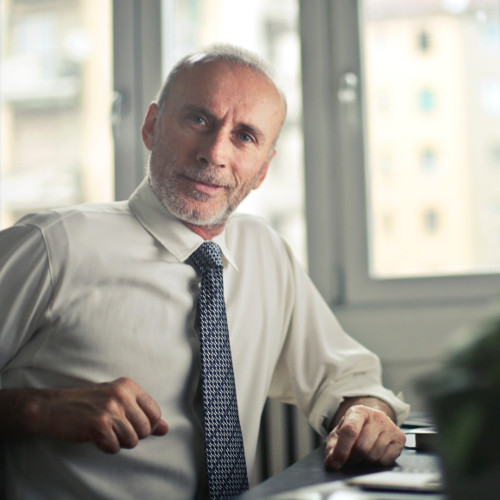
\includegraphics[scale=0.15]{persona_frank}
\caption{Persona --- Frank.}
\label{fig:persona_frank}
\end{figure}

Frank is a hobbyist. He is capable of performing basic computer operations, such as browsing the Internet or using an office suite. Lately, he came across an interesting dataset that highlights population growth in different areas of the world over the past couple centuries. Frank is quite impatient when it comes to computers and gets easily frustrated with complex pieces of software. As such, he is looking for a tool that will enable him to view this data without too much hassle.

\subsection{Power user}

\begin{figure}[ht]
\centering
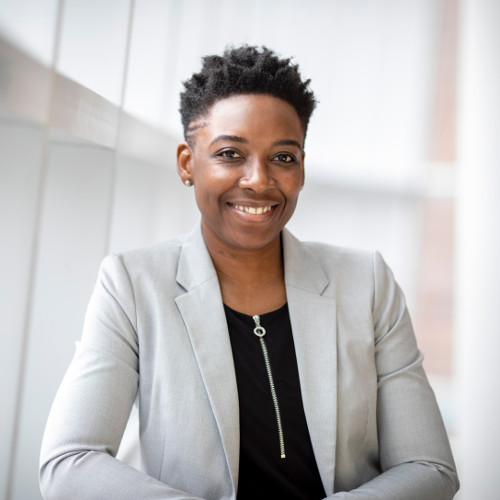
\includegraphics[scale=0.15]{persona_quinn}
\caption{Persona --- Quinn.}
\label{fig:persona_quinn}
\end{figure}

Quinn is a senior data analyst working at a meteorological agency. She possesses advanced programming skills and her current task is to build a networked swarm of drones that gather meteorological data from locations around her neighbourhood. She wants to remotely access the measured data and share measurements from particular days with her colleagues.

\subsection{IT administrator}

\begin{figure}[ht]
\centering
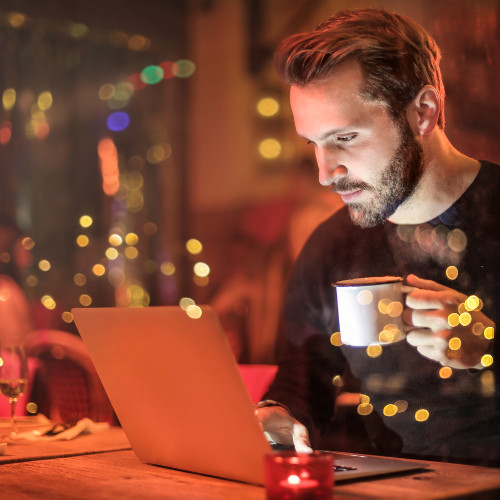
\includegraphics[scale=0.15]{persona_paul}
\caption{Persona --- Paul.}
\label{fig:persona_paul}
\end{figure}

Paul works as an IT technician at a corporate bank. He has been tasked by the company to find and recommend an immersive analytics platform to be used by its employees. Paul wants the software to store data locally in order to achieve compliance with new data regulations, integrate easily with existing processes inside the company and have the ability to audit the software. Although he is an experienced administrator with many years under his belt, he always enjoys software that is hassle-free to run and easy to set up.

\section{Task analysis}

The goal of our research is to create a virtual reality visualization environment that is accessible to everyone, is easily extensible by outside developers and works on 3DOF and 6DOF HMDs, no matter whether they are connected to a personal computer or function as standalone devices. Different control styles should be taken into account when designing interactions. The following graph illustrates tasks that are typical for immersive analytics software (and for the most part, traditional business intelligence tools). High-level tasks are broken down into subtasks as is commonplace in hierarchical task analysis.\autocite{hta}

\begin{figure}[ht]
\centering
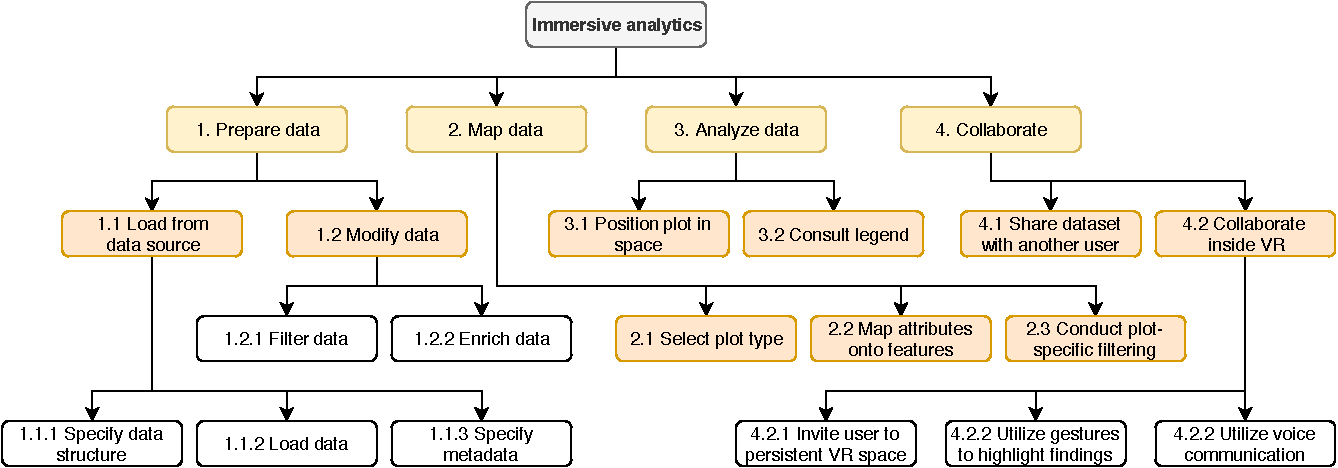
\includegraphics[scale=0.55]{hta}
\caption{Hierarchical task analysis of typical immersive analytics software.}
\label{fig:hta}
\end{figure}

The users typically traverse these tasks in order, however, depending on the scenario, they may want to repeat tasks 2-4. It is important to note, that when collaborating with another user, tasks 1-2 can be skipped. Detailed descriptions of each task follow.

\begin{table}[]
\centering
\caption{Description of tasks in hierarchical task analysis.}
\label{hta-desc}
\scalebox{0.7}{
\begin{tabularx}{\textwidth}{|l|X|}
Task & Description\\
Prepare data & The user has to define the underlying structure of data they want to use. This is typically a local file in a certain format or an API provided by a third-party application. They can then proceed to retrieve such data and specify various associated features (\emph{metadata}), such as attribute types or labels (in case of multivariate data). They are also able to select a subset of data to work with or fill in missing values.\\
Map data & The user makes an informed decision on which plot type they wish to use and associates attributes from their dataset with its features. They are also able to conduct plot-specific filtering (e.g. by modifying the range of displayed values on a spatial axis in scatter plots).\\
Analyze data & This task includes looking at plots from different viewpoints and discovering further information by consulting the legend.\\
Collaborate & Collaboration can be divided into two distinct areas --- synchronous and asynchronous. If the user we are collaborating with is available for real-time collaboration, we can invite them to a persistent virtual space and communicate using voice and physical gestures that map onto our virtual avatars. Alternatively, we are able to send them a copy of our dataset, which they can analyze at their leisure.
\end{tabularx}
}
\end{table}

\section{Scenarios}

Let us specify three scenarios that highlight certain use cases.

\subsection{Loading a dataset from a local file}

Frank opens up the application, logs in and proceeds to add a new dataset representing population growth in the last century. He locates a CSV file on his computer and answers a series of simple questions. After the application finishes loading the dataset, he promptly checks whether the data has been correctly loaded and attribute types correctly assigned. He notices that several attributes have been mistyped as numerical instead of locational and that several attribute labels are ambiguous. He proceeds to fix these issues and puts on a virtual reality headset.

Inside VR, Frank selects the dataset he had just uploaded and creates a globe plot. He assigns locational attributes onto compatible features of the plot and specifies a numerical attribute as value. As Frank rotates the globe, he observes several hotspots around the world --- eastern portions of China catch his eye. He moves the globe closer towards him and continues to explore.

\subsection{Creating an integration}

Quinn has recently finished work on her new fleet of Internet-connected drones. She is using Python to periodically gather measurements of temperature, humidity, wind direction and wind speed. Every day at a set time, the drones travel along a pre-programmed path and log measurements at certain locations. These measurements are then dumped into a file, which is stored in the drone's internal memory. Quinn, wanting to utilize the full capabilities of her drones, decides to add an integration to her Python script. She opens up our application, logs into her account and adds the file containing her last measurements as a new dataset. She then turns on a feature called \emph{version history}, that enables her to upload multiple versions of the same dataset.

Quinn proceeds to look up the API key specific to the dataset she had just added along with instructions on how to set up the Python integration. After installing the integration from Python's package manager, she replaces the bit of code that saves measured data as a file with a snippet that she found. The next day after her drones return from their travels, Quinn notices that a new version of data has been added to her dataset. She puts on her VR headset, creates a map plot and assigns attributes from her dataset onto its features. Quinn then changes between the two versions and can see that today's measurements indicate higher humidity in certain areas as well as a change in wind direction.

\subsection{Collaborating with another user}

Quinn wants to share her findings with her fellow employee, Bob. While in VR, she opens her friends list and notices that Bob is online. She invites him to join her in VR. Bob gets a notification and puts on his VR headset. He accepts the invitation and after waiting several seconds for Quinn's data to load, appears in a shared virtual space beside Quinn's virtual avatar. Quinn then briefs Bob on the current meteorological situation using the application's voice communication functionality. She points to the area of interest and both agree that the situation is unusual. Bob requests a personal copy of the dataset and Quinn is happy to oblige. She takes off her VR headset and sends the dataset to Bob who then receives a prompt to accept the share request.

\section{Design goals}

Let us specify key design goals for our application.

\subsection{Inclusivity}

The application should be accessible to users without any prior experience with data analysis. Workflows that are expected to be utilized by the vast majority of users should be straightforward. More advanced functionality can be available for experienced users, but its presence should not deter newcomers from using the product.

\subsection{Extensibility}

The application has to be extensible to a certain degree as to give stakeholders the ability to integrate it with their existing software stack.

\subsection{Data security}

Users are not to be held hostage inside the application's ecosystem (\emph{vendor lock}). All data should be retrievable with ease by the user and a system administrator where applicable. There should be an option to store data locally without a requirement to connect to outside servers.

\subsection{Collaboration}

The application should facilitate collaboration between multiple users. They should be able to share data with one another without being forced to resort to external tools. In an optimal scenario, they should have the ability to communicate and interact with one another inside the virtual environment.

\subsection{Non-specificity}

Use cases of our application should not be limited to a select field or domain of data.

\subsection{Focus on VR}

The application's user interface should be tailor-made for virtual reality. It is to be designed around a spatial environment while mitigating all shortcomings of present-day virtual reality technology.

\subsection{Availability}

The application is to be available on all major virtual reality platforms across PC, mobile and standalone categories. The user should be able to retain a persistent copy of their data across all devices as they may for instance use a workstation at their workplace and a standalone system at home.

\subsection{Automatization}

When adding a new dataset, the application should be able to predict certain features, such as attribute type or structure of an uploaded dataset. The user should only be prompted if there is a high degree of uncertainty. In the inverse case, we will choose the most likely settings and allow the user to make modifications later at their leisure.

\section{Feature selection}

In this section, we will set the scope of our application by selecting features to meet aforementioned design goals and use cases. The user should be able to load industry-standard comma-delimited (CSV) files into the environment. Two data structures are to be supported --- \emph{multivariate datasets}, which contain multiple attributes arranged in columns and two-dimensional arrays of numerical values, which will be further referred to as \emph{matrix datasets} for the lack of a more suitable term. Multivariate datasets may or may not include attribute labels. If they are present, they should be presented as a comma-delimited list on the first row of the file as per the example below.

\begin{lstlisting}
Sepal length,Sepal width,Petal length,Petal width,Species 
5.1,3.5,1.4,0.2,Iris-setosa
5.6,3.0,4.1,1.3,Iris-versicolor
6.3,3.3,6.0,2.5,Iris-virginica
\end{lstlisting}

\begin{lstlisting}
0.3,0.4,0.6,0.4,0.3
0.4,0.5,0.7,0.5,0.4
0.6,0.4,0.5,0.4,0.6
0.4,0.5,0.7,0.5,0.4
0.3,0.4,0.6,0.4,0.3
\end{lstlisting}

When loading a new dataset into our application, the data type of each attribute should be automatically determined and presented to the user along with an option to change to another type that suits the provided data. In addition, the user should be presented with basic statistical data and data preview, so that they can make an informed decision regarding the data type of each attribute. The specifics of each attribute type are discussed later in this section. Users should also be able to change the label of each attribute and decide on how to fill in missing values.

The user should be able to load a new version of the dataset, provided the data structure meets dataset specifications. They are to be given an option to replace existing data or add a new \emph{version}. In the latter case, the user will have the ability to change between versions when visualizing data from said dataset.

When in VR, the user will be able to choose between five types of plots discussed below, position them freely around the virtual environment, adjust their rotation and scale, assign dataset attributes onto features of the plot and view basic dataset metadata and statistics of attributes contained within said dataset. The user should also be able to filter by attribute value, regardless of whether said attribute is assigned onto a feature of the plot.

Collaboration features should include the ability to share datasets with another user directly within the environment and also the ability to invite said user to a shared virtual environment with users represented as articulated virtual avatars that are capable of moving in space and voice communication.

Lastly, there should be integration support for popular programming languages that allows programmers to create or update datasets from their programming environment of choice. Since we cannot cater to all, we should provide the ability for outside developers to build their own integrations for other programming languages or environments.

\subsection{Plot types}

In order to satisfy the non-specificity design goal, we have to offer the user a variety of plot options. Six plot types were selected for implementation, four for multivariate and two for spatial data (matrix datasets).

\begin{figure}[ht]
\centering
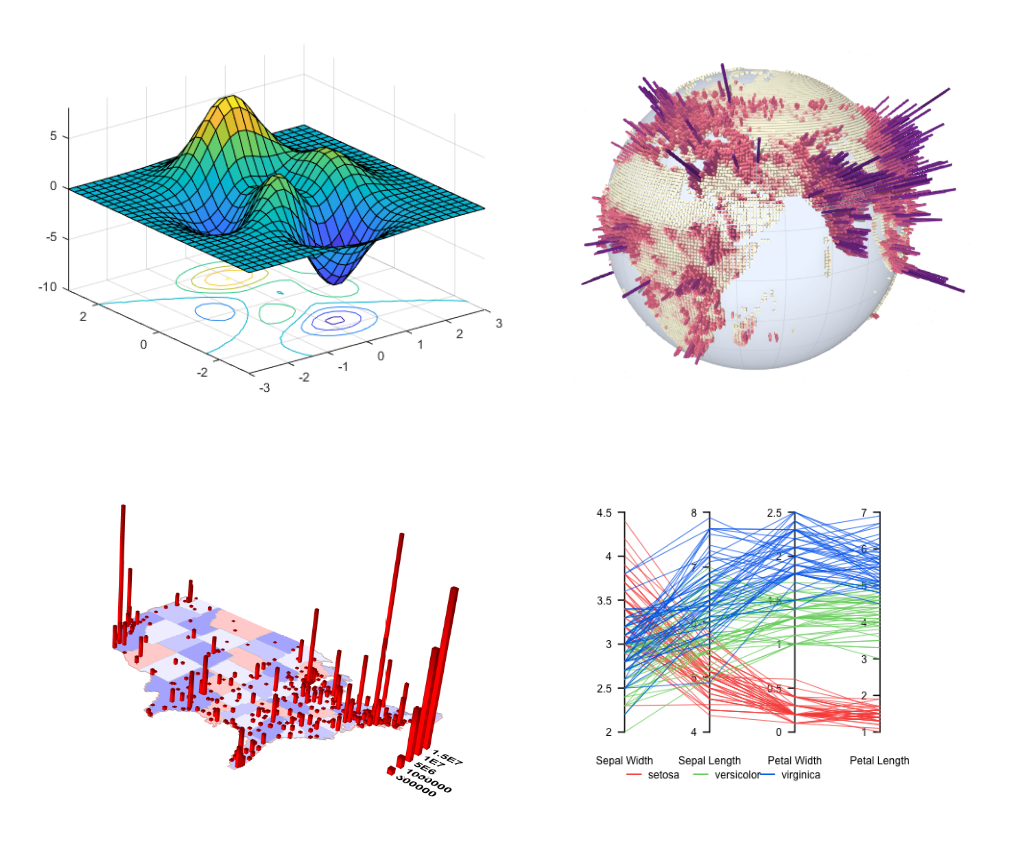
\includegraphics[scale=0.2]{plot_types}
\caption{Clockwise from top left: surface plot, globe plot, scatter plot, bar plot, parallel coordinates plot, map plot.}
\label{fig:plot_types}
\end{figure}

\subsubsection{Scatter plot}

Accepts multivariate data. Allows the user to assign numerical values onto spatial axes, which determine the position of the nodes. Spatial axes also allow for the assignment of categorical attributes, however the ordering in this case is non-deterministic. The user is able to specify bounds for each axis. Assignable non-spatial features include color, size, shape and label, which is set to appear when the user points at a node.

Color mapping differs based on the type of the assigned attribute. Numerical attributes map onto a gradient, which can be diverging (if the attribute includes both positive and negative numbers) or sequential (otherwise). When assigning a categorical attribute, each unique value is given a color with distinct hue. Size only accepts numerical attributes. Shape accepts either numerical or categorical attributes. In the former case, the values are divided into two bins of a similar size with median used as the division point, each half is then rendered as a different glyph. In the latter case, we try to map each unique value onto a distinct glyph. If the number of distinguishable glyphs is smaller than the number of unique values, one of the glyphs can substitute a greater number of unique values.

\subsubsection{Globe plot}

Accepts multivariate data. The globe plot accepts two locational attributes for coordinates (latitude, longitude) and a single numerical or categorical attribute. If a numerical attribute is assigned as a value, it renders bars that protrude from the globe. Assignment of a categorical attribute will result in the rendering of uniformly-sized marks of different colors, the hue of which is again distinct for each unique value.

\subsubsection{Map plot}

Accepts multivariate data. A flat version of the globe plot suitable for viewing smaller geospatial areas.

\subsubsection{Parallel coordinate plot}

Accepts multivariate data. Contains two or more axes, each of which represents a numerical or categorical attribute. A polyline is then created between the axes with vertices positioned in the same way as values on a spatial axis of a scatter plot. The user is able to position the axes around the space using an interaction technique borrowed from a distinguished paper.\autocite{imaxes}

\subsubsection{Surface plot}

Accepts spatial data. Renders a continuous mesh, the elevation of which is determined by numerical values at a specified position in the two-dimensional matrix.

\subsubsection{Bar plot}

Accepts spatial data. Renders a series of bars, with their height determined in the same way as with the surface plot.

\begin{figure}[ht]
\centering
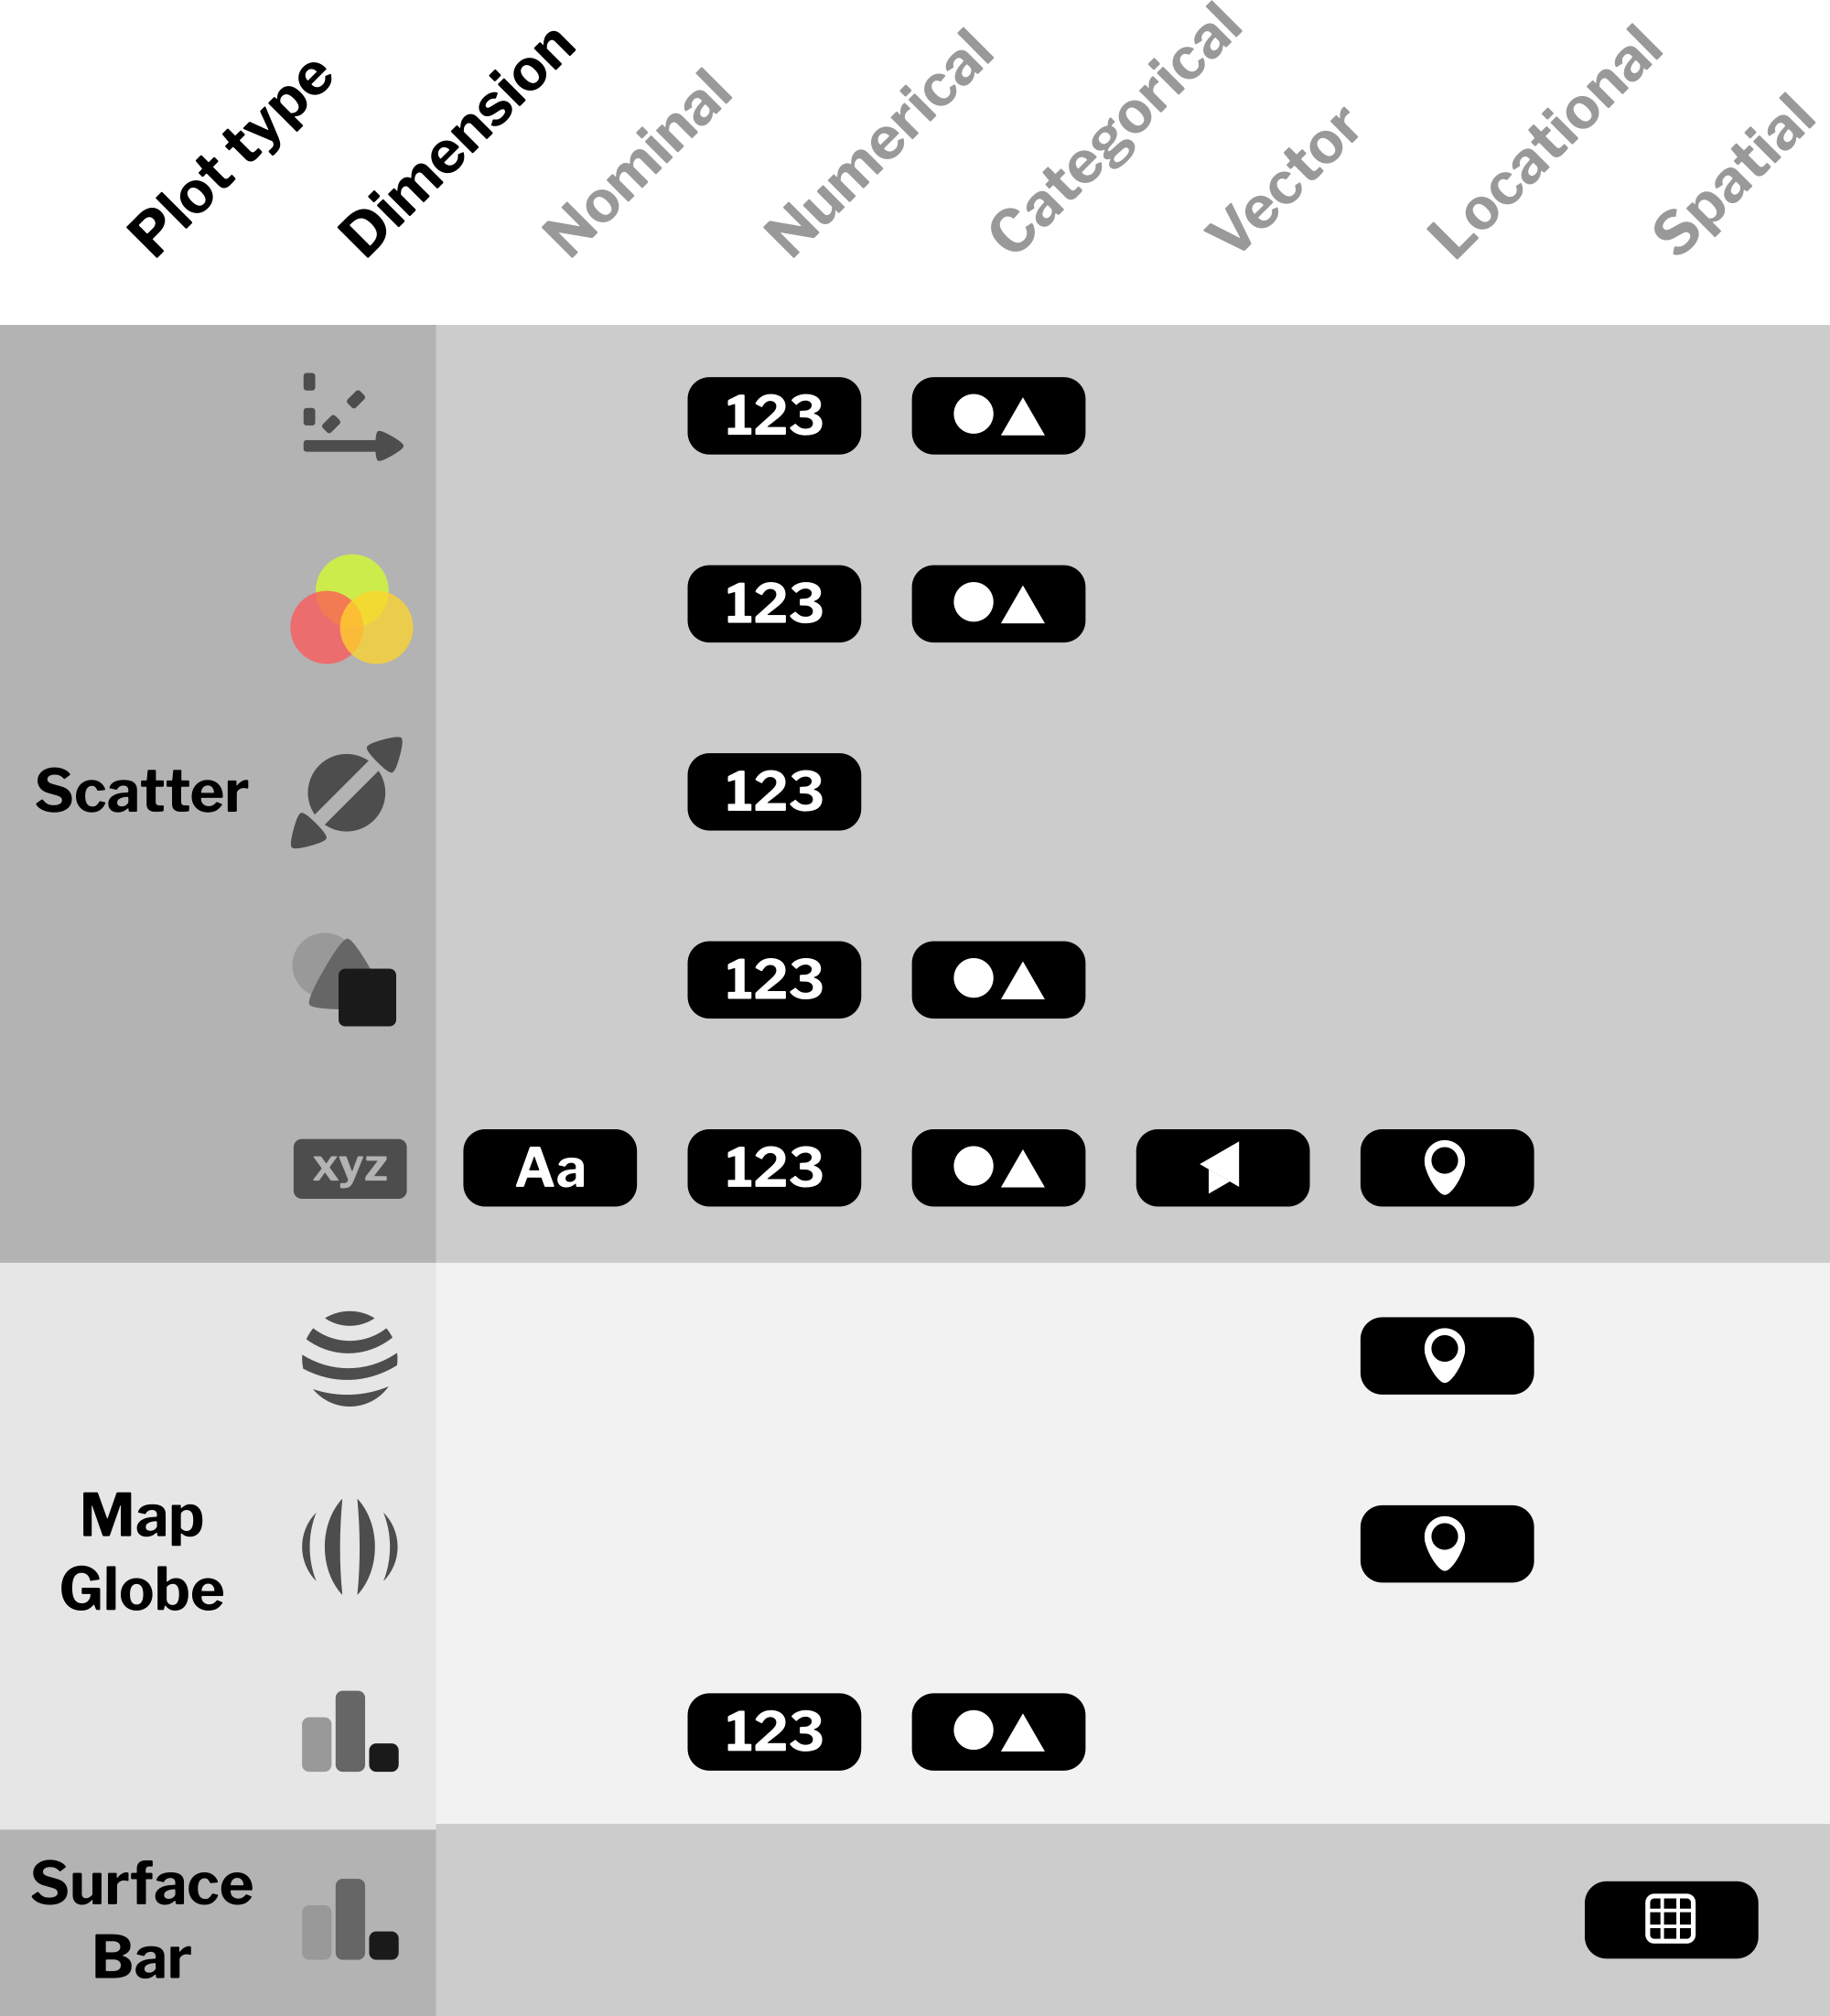
\includegraphics[scale=0.06]{type_matrix}
\caption{Type compatibility with different features of each plot.}
\label{fig:type_matrix}
\end{figure}

\subsection{Attribute types}

This subsection lists attribute types to be supported by our application. As mentioned earlier, an attribute type is automatically assigned when loading a new dataset. The user is then given the ability to change to any other type provided the attribute in question meets the type's requirements. Flow of the auto-assignment process is detailed by the following decision tree.

\begin{figure}[ht]
\centering
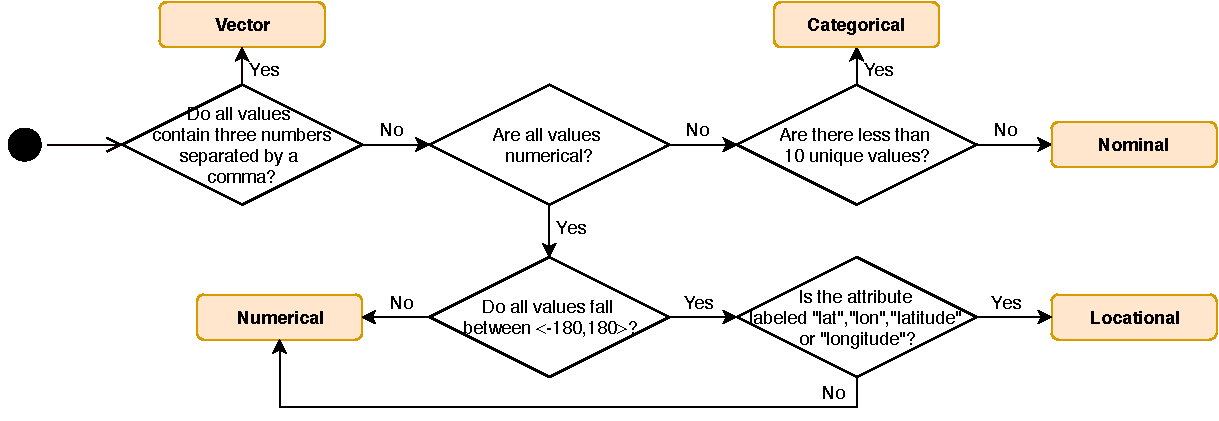
\includegraphics[scale=0.6]{attribute_assignment}
\caption{Decision tree for automatic assignment of attribute types in multivariate datasets.}
\label{fig:attribute_assignment}
\end{figure}

\newpage

\subsubsection{Nominal}

Nominal attributes do not have any special requirements. Attributes default to this type should they fail all other assignment checks.

\subsubsection{Numerical}

Numerical attributes represent numbers in both decimal and integer formats. Decimal point is to be represented by a dot. The type is automatically assigned if all of the attribute's values are numeric and do not satisfy conditions set for the locational type.

\subsubsection{Categorical}

Categorical attributes do not have any special requirements. The type is automatically assigned if the attribute in question has less than 10 unique values, where 10 is an arbitrary number chosen by the author.

\subsubsection{Vector}

Vector type is designed for storing three-dimensional vectors. The accepted format is specified as three numerical values separated by spaces. If all values of a specific attribute adhere to this convention, the type is automatically assigned.

\subsubsection{Locational}

Locational type is a subset of the numerical type representing geospatial coordinates. Decimal values between --180 and 180 are permitted. The full range is used to represent longitude, while a reduced range from --90 to 90 represents latitude. An attribute is automatically determined to be spatial if it meets the requirements and is labeled as one of the following (case-insensitive):

\begin{itemize}
\item latitude,
\item longitude,
\item lat,
\item lon
\end{itemize}

\subsubsection{Spatial}

Spatial type is exclusive to matrix datasets, where it represents the sole “attribute” containing all data. It is automatically assigned and cannot be changed by the user. As it only supports numerical data, datasets that do not satisfy this condition will be treated as multivariate instead.

\section{Component design}

Two big issues in present-day virtual reality technology that we would like to focus on are low pixel density of displays on most consumer HMDs compared to modern computer monitors and non-intuitiveness of text input in VR. The first fact leads to poor legibility of text below a certain size. This effect is compounded in HMDs with an OLED screen, due to their characteristic pentile subpixel arrangement. Text input in VR typically consists of pointing the controller towards a virtual keyboard, the layout of which is reminiscent of its smartphone variant. Using such keyboard for a short amount of time is a mere inconvenience, attempting to do so for longer periods of time will lead to fatigue, due to the need to precisely position a controller in space.

\begin{figure}[ht]
\centering
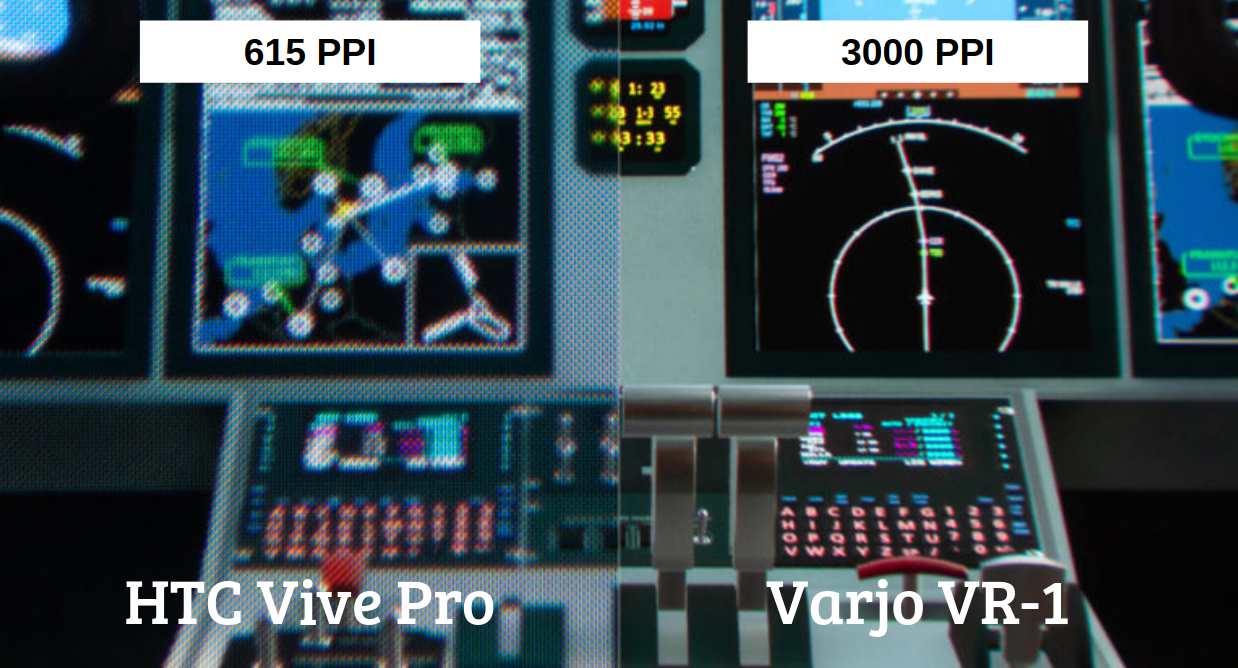
\includegraphics[scale=0.2]{pixel_density}
\caption{Comparison of pixel density between a high-end consumer headset and a business-oriented HMD.\autocite{varjocomparison}}
\label{fig:pixel_density}
\end{figure}

Over the years, there have been many attempts to come up with a solution that mitigates the fatigue, one of which is a project called Punchkeyboard.\autocite{punchkeyboard} We had originally planned on designing a similar solution, however doing so would only work in 6DOF, requiring us to use a traditional keyboard interface in 3DOF. In order to alleviate both these issues, we came up with a component design, which divides the overall workflow --- text input is done inside a WIMP interface on the computer, allowing the user to use the computer keyboard they are most likely already familiar with. Furthermore, usage of text in the VR part of our application is greatly reduced in favor of using icons.

\begin{figure}[ht]
\centering
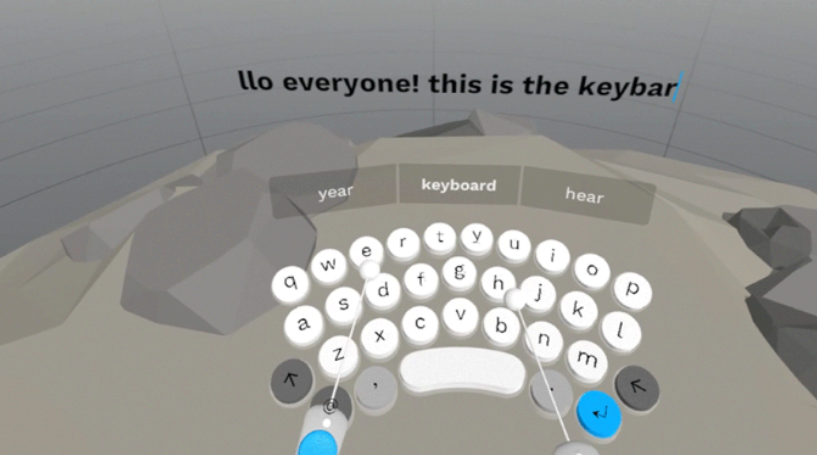
\includegraphics[scale=0.4]{punch_keyboard}
\caption{Example use of Punchkeyboard.\autocite{punchkeyboard}}
\label{fig:punch_keyboard}
\end{figure}

The three distinct components that we have chosen to divide our environment into are as follows --- plugins, Manager and Navigator. \emph{Plugins} are API integrations written for different programming languages that allow the user to create a new dataset or update an existing one. \emph{Manager} enables the user to view and edit all of their datasets and also facilitates loading files from the local computer. \emph{Navigator} allows the user to interact with their data in virtual reality. The following visualization pipeline shows the distribution of tasks among our components.

\begin{figure}[ht]
\centering
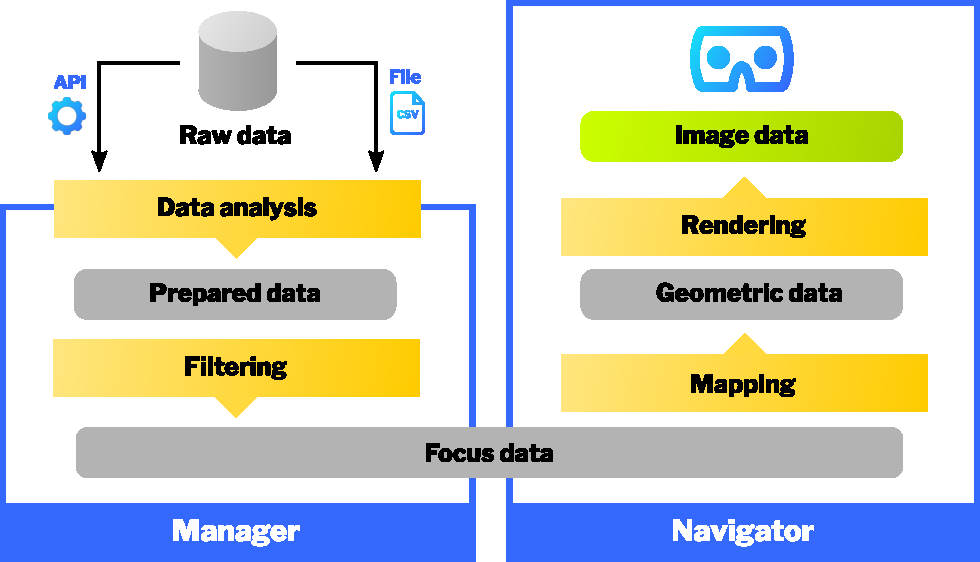
\includegraphics[scale=0.6]{pipeline}
\caption{Adapted version of Haber–McNabb dataflow model for scientific visualization in the context of our environment.\autocite{santos}}
\label{fig:pipeline}
\end{figure}

\section{Challenges of VR design}

The spatial nature of virtual reality applications carries with it certain design challenges, which make it difficult to utilize the typical prototyping workflow. As interaction techniques in VR are much more complex than in typical WIMP applications, we are unable to create a rich interactive prototype without being forced to delve into code. The typical workflow for VR prototyping consists of drawing sketches, creating 2D and 3D assets that we intend to use in our project and then positioning said assets inside a \emph{static} 3D environment (\emph{spatial prototyping}). The user is then able to move between these scenes and also in 3D space, but they are unable to interact with any of the objects.\autocite{vrprototyping} Commonly used tools for spatial prototyping include Google Blocks\autocite{googleblocks} and Microsoft Maquette\autocite{msmaquette}. We will be using the latter as it is the more advanced of the two.

When it comes to our workflow, we will begin by creating a sketch of basic interactions. This is key, as the design of our user interface greatly depends on limitations imposed by the interaction scheme that we are going to use. We will follow up by creating a UI design for our application, which will share its design language with Manager, allowing for a consistent experience. Afterwards, we will alternate between designing prototypes in Maquette and implementing new features in our game engine of choice. After each run, we gather user feedback and attempt to incorporate it into our design.

\chapter{Manager}

\begin{figure}[ht]
\centering
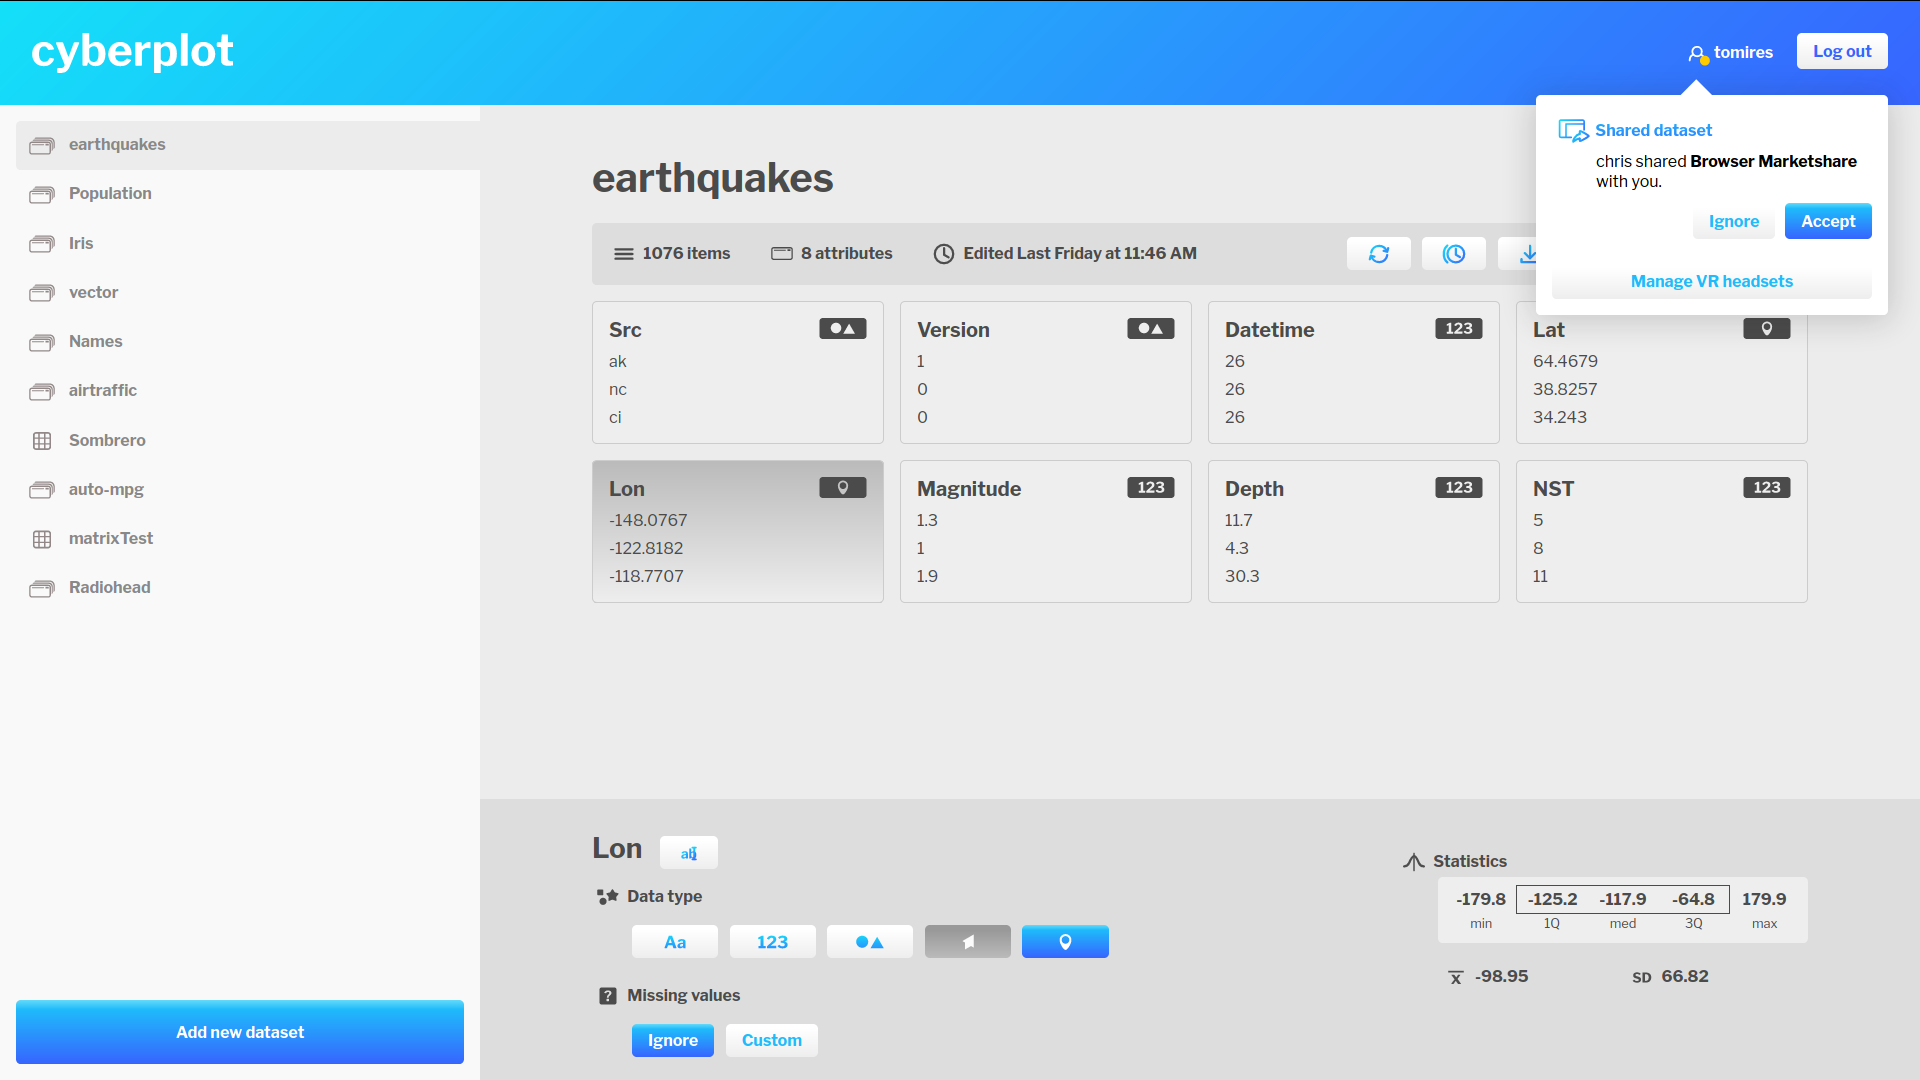
\includegraphics[scale=0.2]{manager}
\caption{User interface of Manager.}
\label{fig:manager}
\end{figure}

Manager is the name for a component which enables the user to load datasets from their local computer and perform basic editing operations, such as data enrichment and attribute specification. In order to satisfy the design goal of mitigating all shortcomings of VR (\emph{Focus on VR}), we have created a separate component that is accessible from a personal computer. Facilitation of collaboration, another of our design goals, demands that we create a centralized server node. 

This backend will provide the users with a user account as well as a space to store all of their datasets and associated metadata. The design goal of availability mandates that the VR portion of our application suite should be made available on mobile and standalone headsets, as well as PC-based systems. As such, we had to figure out a way to access the data on any computer --- an elegant solution is to create a web-based frontend.

To simplify our component design, we will use the term \emph{Manager} to refer to both backend and frontend portions of this application, even though they are separate implementation-wise. Extensibility and data security will be achieved by open-sourcing the component, which enables outside developers to create integrations (\emph{plugins}) and other stakeholders to audit the software.

\section{Required functionality}

Users should be able to do the following:

\begin{itemize}
\item create a user account,
\item upload new datasets,
\item access previously uploaded datasets,
\item download previously uploaded datasets,
\item update an existing dataset,
\item change attribute types,
\item rename attribute labels and datasets,
\item share datasets,
\item delete datasets
\end{itemize}

\section{Wireframes}

We began our design process by creating wireframes of the user interface. Two versions have been designed, the first consists of two separate views. The first view includes a listing of all uploaded datasets along with basic metadata --- time of the last edit and users the dataset has been shared with. The presentation is reminiscent of folder listing in Google Drive.\autocite{gdrive} The second view contains basic dataset metadata along with a selection of dataset-specific actions on the right-hand side. Data preview contains a histogram where applicable and a complete listing of data. It has been inspired by the UI of Kaggle.\autocite{kaggle} Attribute-specific changes would have taken place inside a modal.

\begin{figure}[ht]
\centering
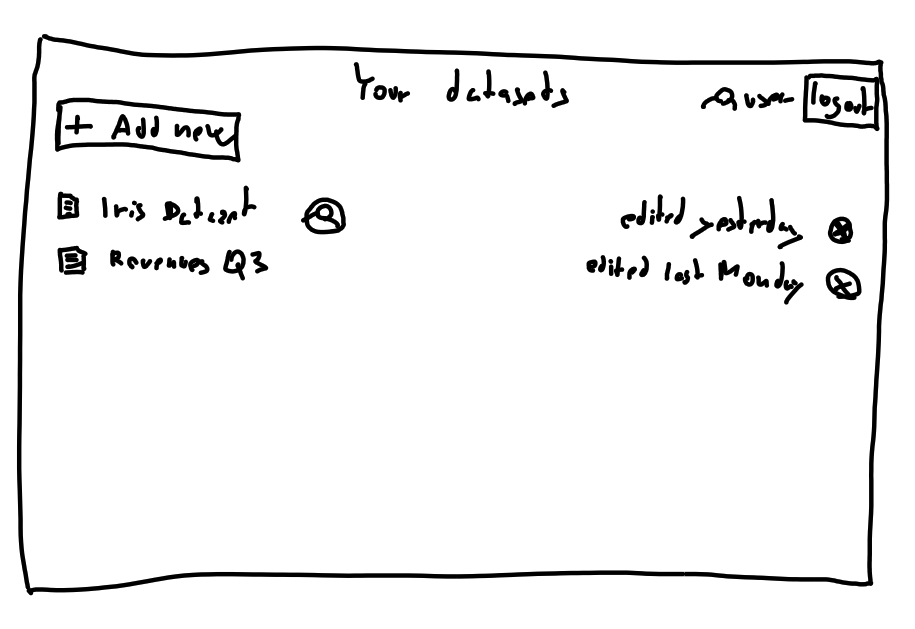
\includegraphics[scale=0.2]{wireframe_dataset1_1}
\caption{Wireframe of Manager's interface (version 1) --- dataset listing.}
\label{fig:wireframe_dataset1_1}
\end{figure}

\begin{figure}[ht]
\centering
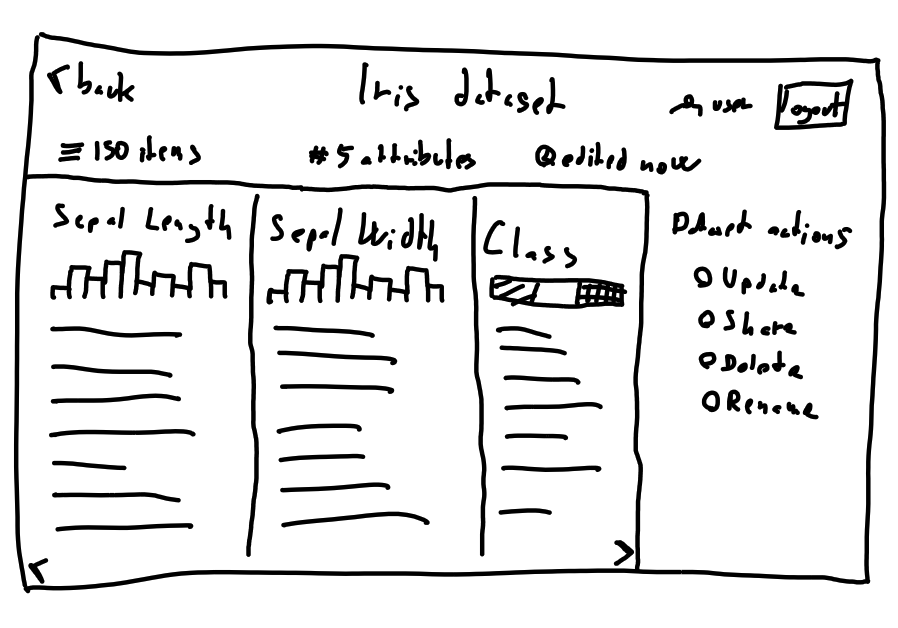
\includegraphics[scale=0.2]{wireframe_dataset1_2}
\caption{Wireframe of Manager's interface (version 1) --- dataset view.}
\label{fig:wireframe_dataset1_2}
\end{figure}

The second version includes a more compact interface with a listing of datasets in a sidebar on the left, dataset information in the center and attribute-specific information in the bottom-right portion of the screen. Dataset-specific actions are accessible in the upper portion of the screen, followed by the listing of attributes, which use design consistent with the data panel in Navigator.

\begin{figure}[ht]
\centering
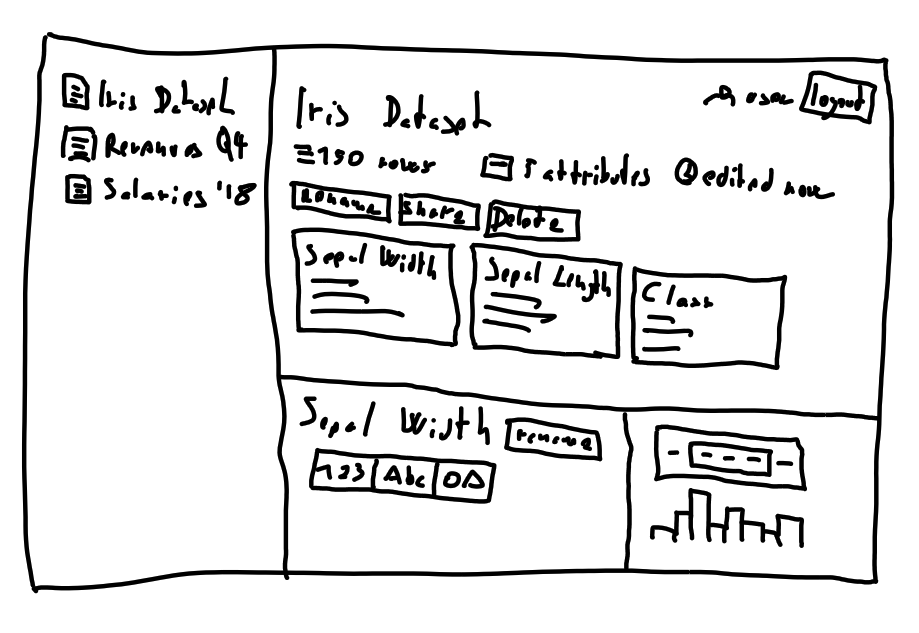
\includegraphics[scale=0.2]{wireframe_dataset2}
\caption{Wireframe of Manager's interface (version 2).}
\label{fig:wireframe_dataset2}
\end{figure}

Most interaction takes place in modals, the following wireframe illustrates the process of adding a new dataset from local file. In accordance with the design goal of automatization, the user is only asked to input necessary information --- in our case the user has to select whether headers are present in the file.

\begin{figure}[ht]
\centering
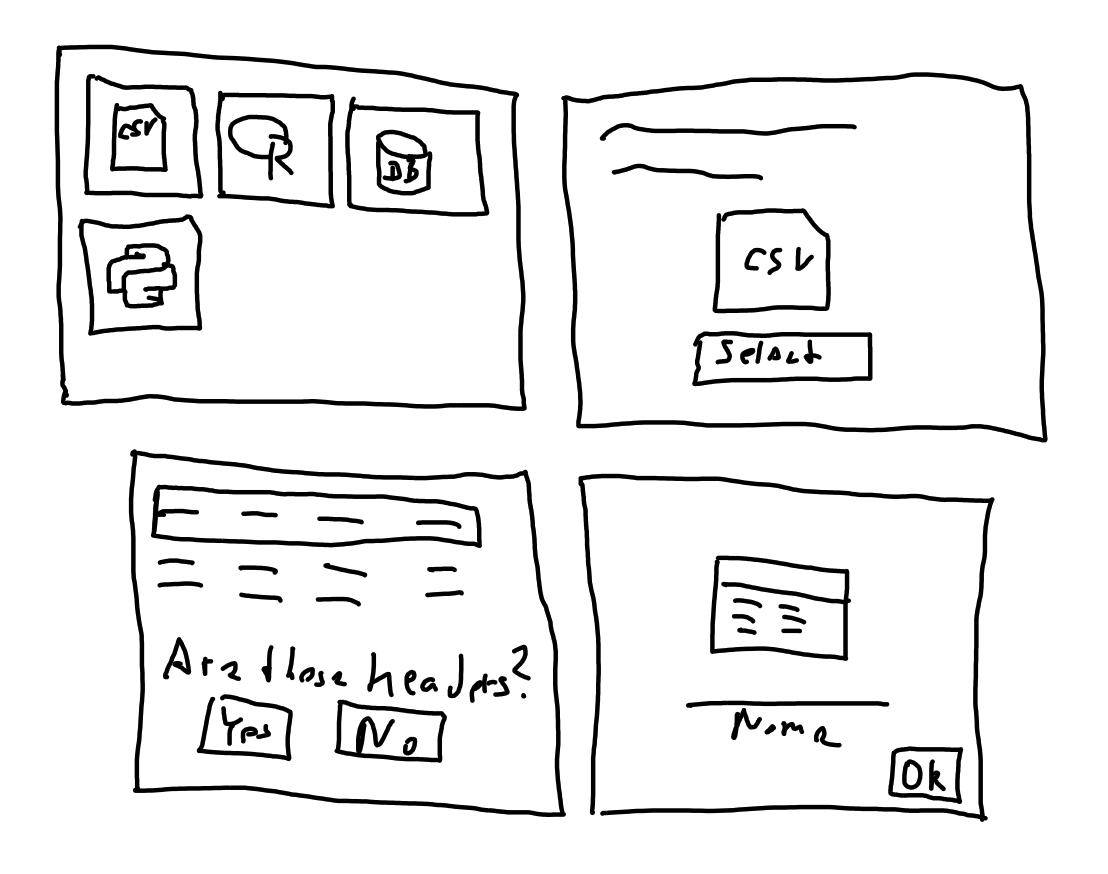
\includegraphics[scale=0.2]{wireframe_upload}
\caption{Wireframe detailing the process of uploading a new dataset from local file.}
\label{fig:wireframe_upload}
\end{figure}

\section{Design stage}

In this stage, we have created a low-fidelity prototype of our user interface based on the second version discussed earlier. Inkscape vector imaging software was used.\autocite{inkscape} The full version of the low-fidelity design is included with this thesis as a digital copy.

\begin{figure}[ht]
\centering
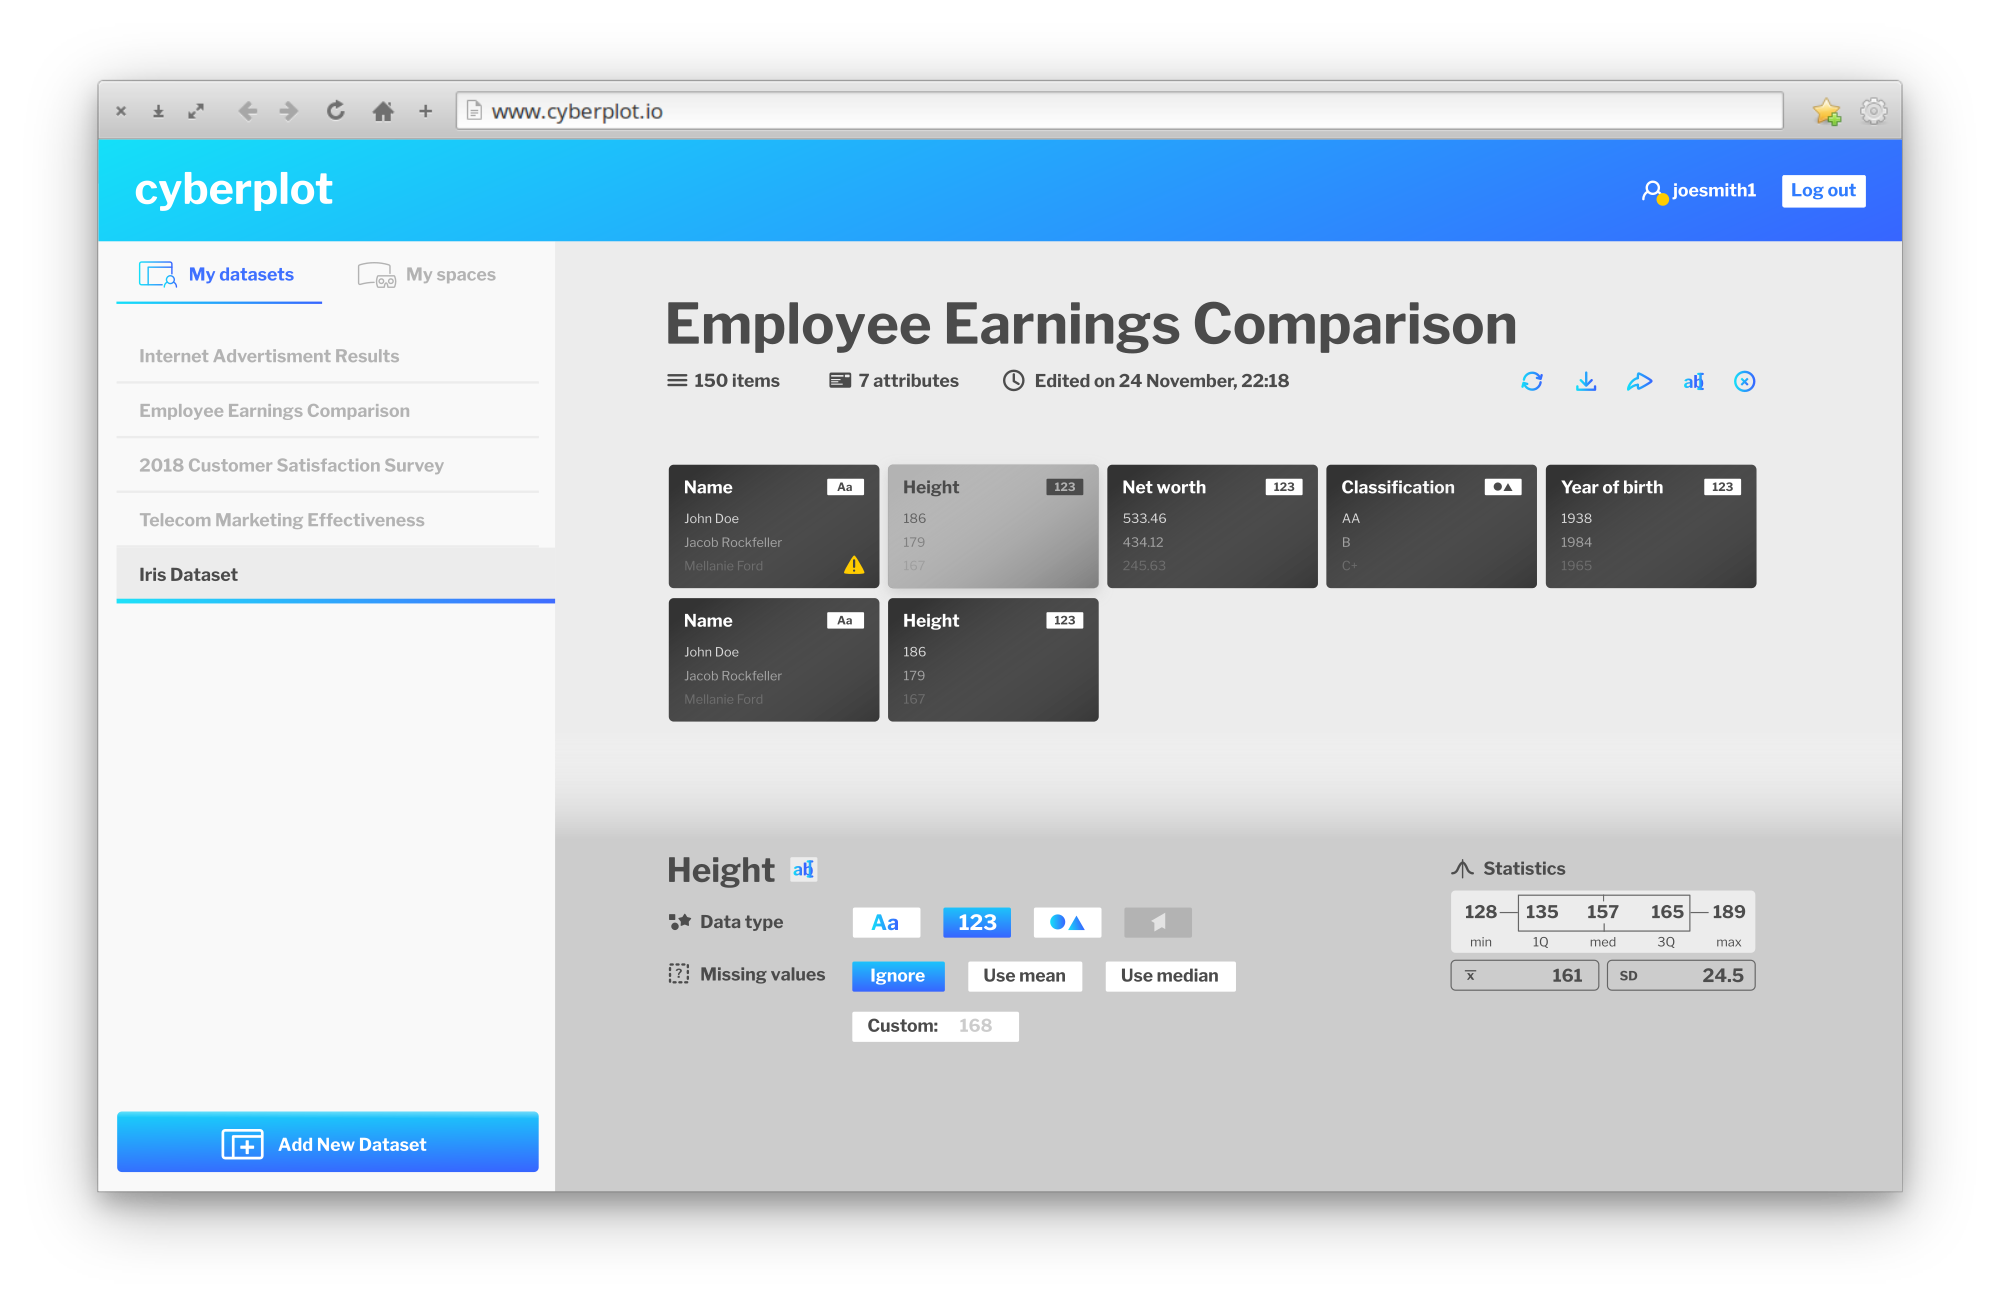
\includegraphics[scale=0.3]{manager_lofi}
\caption{Low-fidelity prototype made in Inkscape.}
\label{fig:manager_lofi}
\end{figure}

\section{Implementation}

The next stage included implementation of the component using Flask\autocite{flask} and Vue.js\autocite{vuejs} frameworks. Details are available in the chapter discussing used technology. The following two subsections include an overview of functionality available inside Manager.

\subsection{August build}

As Manager is a multi-user application, the user first has to create an account. After logging in, they are presented with a list of their datasets on a sidebar to the left. In the upper right corner of the screen, they can see their username and access a notification center, which is where they are able to answer share requests and, most importantly, access the VR headset management window. This window gives them information on headsets associated with their account, such as an identifier (name of HMD as well as the computer's domain name if provided by host OS) and time of association.

In the lower left corner is a button titled \emph{Add new dataset}. Pressing it opens up a wizard for adding a dataset. The same wizard with slight differences is also used when updating an existing dataset. In the first step, the user can select their data source. If they choose a programming environment, they receive instructions on how to use the plugin system.

\begin{figure}[ht]
\centering
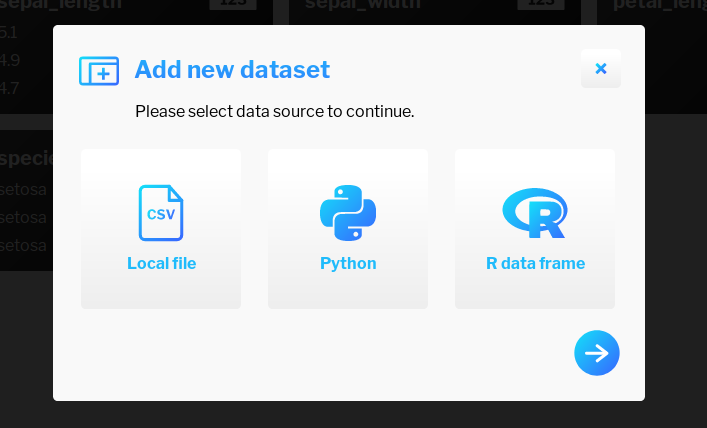
\includegraphics[scale=0.4]{manager_add}
\caption{Options for adding a dataset.}
\label{fig:manager_add}
\end{figure}

\newpage

If they choose to create a dataset from a local file, they are prompted to select a CSV file by either opening an OS-native file picker dialog or by dragging a file icon into their web browser. In the next step, they have to decide whether the first line of their file includes labels. After selecting an appropriate answer, the dataset is uploaded and appears in the sidebar. Attribute types are assigned automatically.

\begin{figure}[ht]
\centering
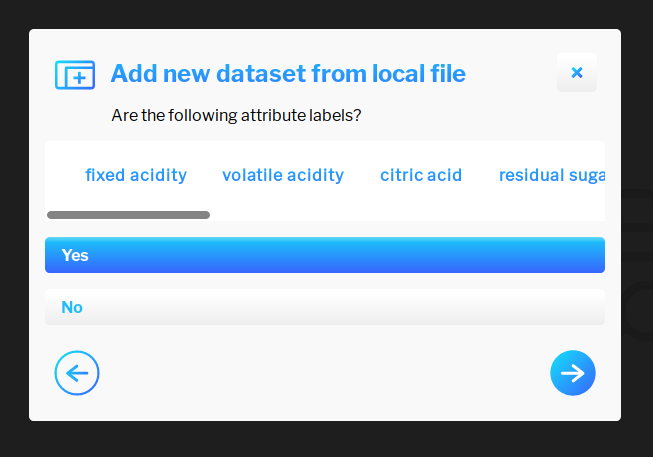
\includegraphics[scale=0.4]{manager_labels}
\caption{Dataset addition wizard.}
\label{fig:manager_labels}
\end{figure}

Clicking on a dataset in the sidebar brings up the dataset view, which contains select metadata (number of attributes, row count, timestamp of last edit), buttons for accessing various functions and a listing of all attributes. For each attribute, we can see its label, data type and a preview of its values. Clicking on an attribute brings up the attribute view that contains options to rename an attribute, change its data type (nominal, numerical, categorical, vector) and decide on which action to take in case some values are missing. With numerical attributes, we are able to view select statistical information, such as quartiles, mean and standard deviation.

If we return back to dataset-wide actions, we have the following options:

\begin{itemize}
\item update dataset,
\item manage dataset versions,
\item download dataset file,
\item share dataset with another user,
\item rename dataset,
\item delete dataset
\end{itemize}

\begin{figure}[ht]
\centering
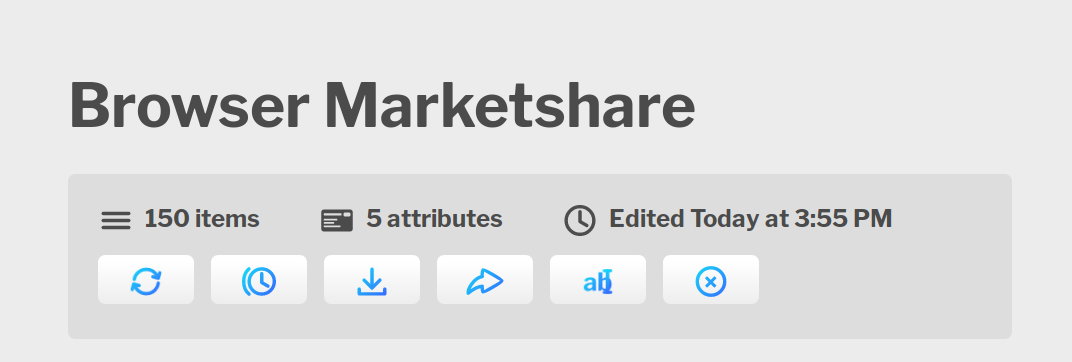
\includegraphics[scale=0.3]{manager_actions}
\caption{Dataset actions. From left: Update, manage versions, download, share, rename, delete.}
\label{fig:manager_actions}
\end{figure}

Sharing a dataset allows us to select a user with whom to share. The next time they log in, they are presented with a notification that enables them to either accept or decline the share request. Should they accept, the dataset is copied onto their account.

Datasets can be updated in the same way as they are created, that is using a local file or via the plugin system. The system checks for any type discrepancies and will refuse upload of data incompatible with current attributes. By default, existing data is overwritten on update. However, we can choose to enable versioning in order to keep multiple copies of the same dataset, essentially adding a temporal dimension to our data. Examples of using this feature include a smart device for gathering data, which periodically uploads said data using the plugin system. Versions can be individually downloaded and deleted using the version management interface. Versioning can also be turned on or off on a per dataset basis.

\begin{figure}[ht]
\centering
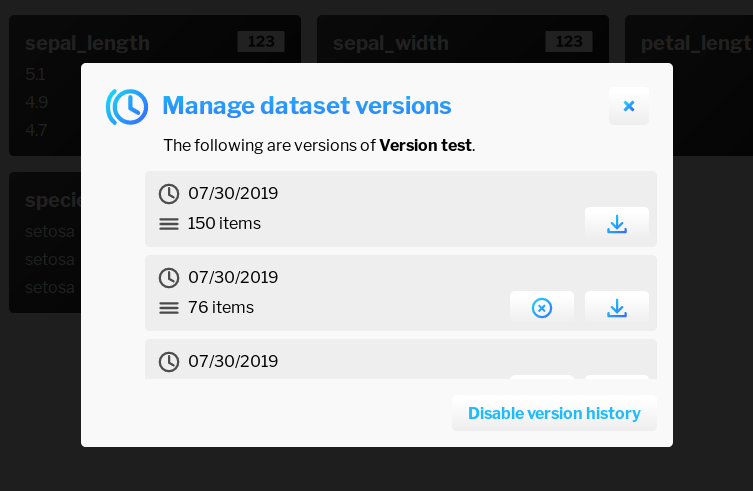
\includegraphics[scale=0.4]{manager_versions}
\caption{Version management in Manager.}
\label{fig:manager_versions}
\end{figure}

\subsection{December build}

The December build of Manager includes the addition of a new attribute type for storing locations, a brand new installation script that allows the administrator to install from source code using a single command as well as a number of bug fixes.

The most significant feature is support for spatial datasets. When adding all-numeric datasets, the user is asked to select whether the dataset in question is multivariate or spatial. Spatial datasets are compatible with certain plots inside Navigator, in both components they are represented as a single unified attribute with a special type.

\begin{figure}[ht]
\centering
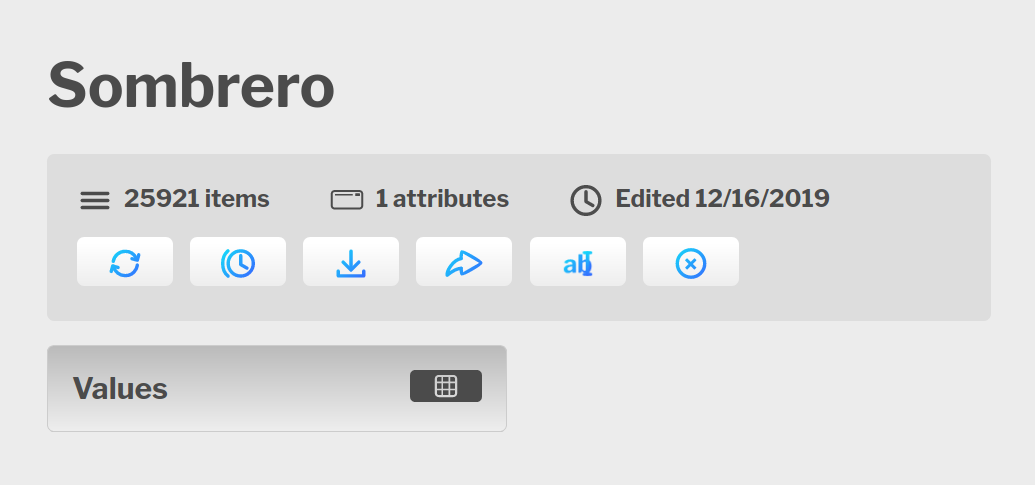
\includegraphics[scale=0.35]{manager_matrix}
\caption{A spatial dataset in Manager.}
\label{fig:manager_matrix}
\end{figure}

\chapter{Plugins}

Plugins are intended for developers or power users to incorporate dataset creation and updating functionality into their applications and scripts. We have implemented integrations for Python and R, as they are the most commonly used programming languages by data scientists. Manager provides a set of APIs that enable outside developers to create their own integrations and as both Manager and official plugins are open-source\autocite{github}, it is a very straightforward process.

\begin{figure}[ht]
\centering
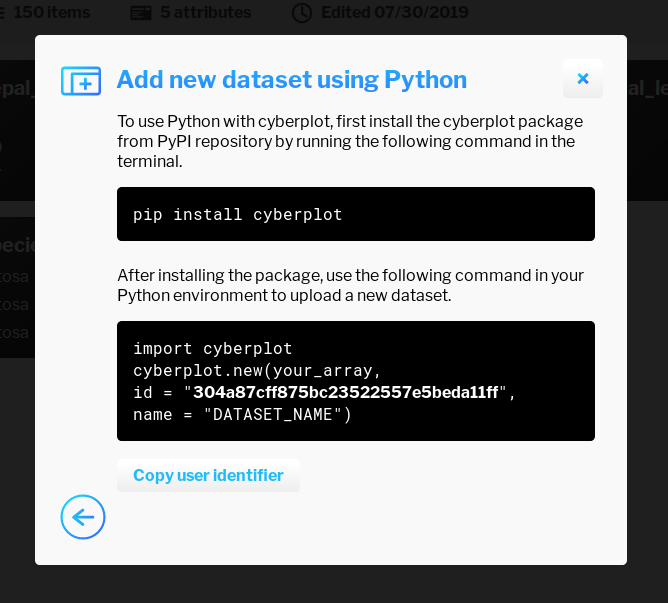
\includegraphics[scale=0.4]{manager_python}
\caption{Guide for adding a dataset using Python.}
\label{fig:manager_python}
\end{figure}

From the user's perspective, the workflow to add or update a dataset is as follows:

\begin{enumerate}
\item Log into Manager.
\item Access the create/update dataset modal.
\item Select programming language or environment.
\item Copy API key that is unique for user (when creating a dataset) or dataset (when updating an existing dataset).
\item Import a library in the programming environment of choice.
\item Insert an applicable command.
\item Run your program.
\end{enumerate}

The following code snippet showcases the use of plugins for adding a new dataset and updating an existing one in R.

\begin{lstlisting}
cyberplot.new(swiss, id = "304a87cff875bc23522557e5beda11ff", name = "Swiss Dataset")
cyberplot.update(iris3, id = "09fee44cff6a79cdf2a6176b2ffb1008")
\end{lstlisting}

The December update adds an option to upload compatible data in the form of matrix datasets by specifying an optional parameter. This opens up the possibility for visualizing mathematical functions using surface plots by first creating their discrete approximations and uploading them as a spatial dataset.

\begin{lstlisting}
cyberplot.new(data, id = "304a87cff875bc23522557e5beda11ff", name = "Matrix dataset", matrix = TRUE)
\end{lstlisting}

\chapter{Navigator}

Navigator is the name for the virtual reality component of our application. It is designed to be used in a wide variety of headsets, including mobile, standalone and PC-based systems, and support both 3DOF and 6DOF tracking.

The original intent was to design two different versions of the application, one with support for room-scale interactions (for 6DOF headsets) and a scaled-down version for 3DOF headsets, however we have decided later in the design process to combine the two as the room-scale version required physical movement between plots, which are distributed around the space. This was deemed uncomfortable and the two versions were merged into one. There are minor differences in both the user interface and user experience between the two, but the basic interaction methods remain the same.

\section{Required functionality}

Users should be able to do the following:

\begin{itemize}
\item associate Navigator with their account,
\item access datasets previously uploaded with Manager,
\item create plots detailed in the design chapter,
\item assign attributes onto plots,
\item conduct basic data filtering,
\item position plots in space,
\item view statistics,
\item collaborate with other users using avatars
\end{itemize}

\section{Interaction design}

We began the design process by creating sketches that highlight interaction techniques used within Navigator. Let us start by introducing the two pivotal user interface elements --- the attribute and the plot. The attribute element displays the label, type of the attribute as well as a data preview.

\begin{figure}[ht]
\centering
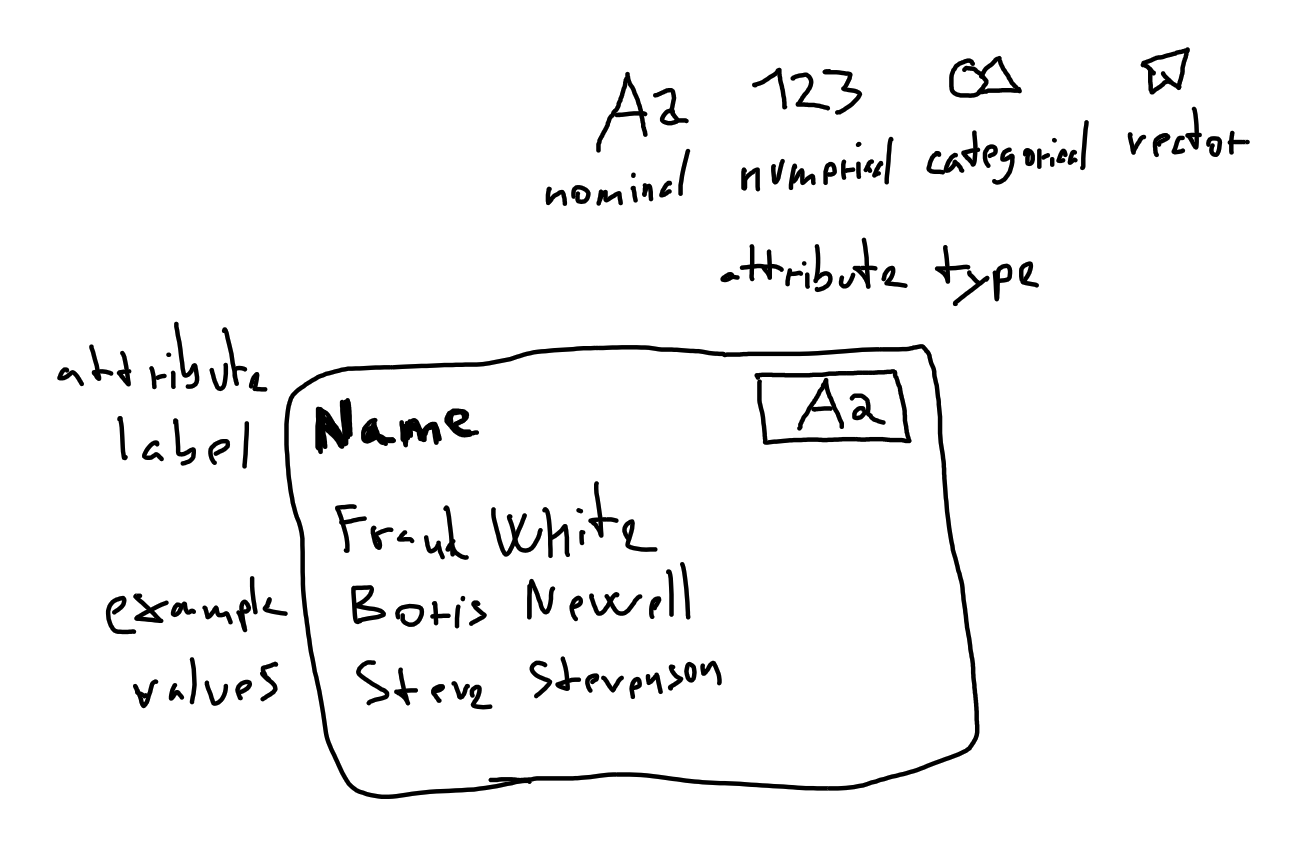
\includegraphics[scale=0.7]{sketch_attribute}
\caption{Attribute element in VR.}
\label{fig:sketch_attribute}
\end{figure}

Plots can be positioned around the user and depending on plot type, a number of features can be assigned to. As discussed previously, the scatter plot accepts assignments to its spatial axes and four non-spatial features --- color, size, shape and label. Assignments are made by dragging the attribute from the data panel onto the feature label. Four shapes were designed for use as glyphs in scatter plots. The following 3D shapes have been selected due to their geometry, which is recognizable from every angle.

\begin{figure}[ht]
\centering
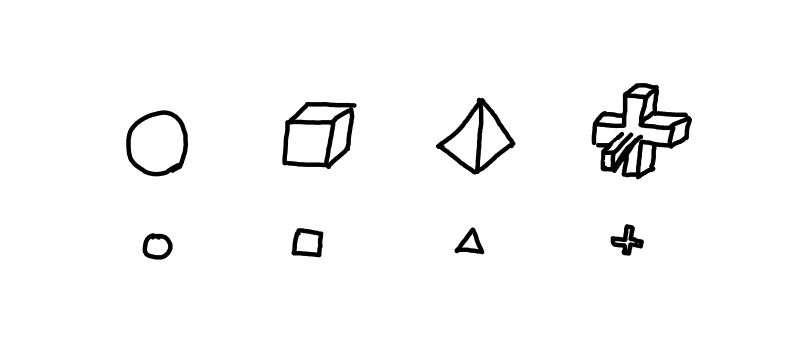
\includegraphics[scale=0.75]{sketch_shapes}
\caption{2D and 3D variants of shapes used in scatter plots.}
\label{fig:sketch_shapes}
\end{figure}

\newpage

\begin{figure}[ht]
\centering
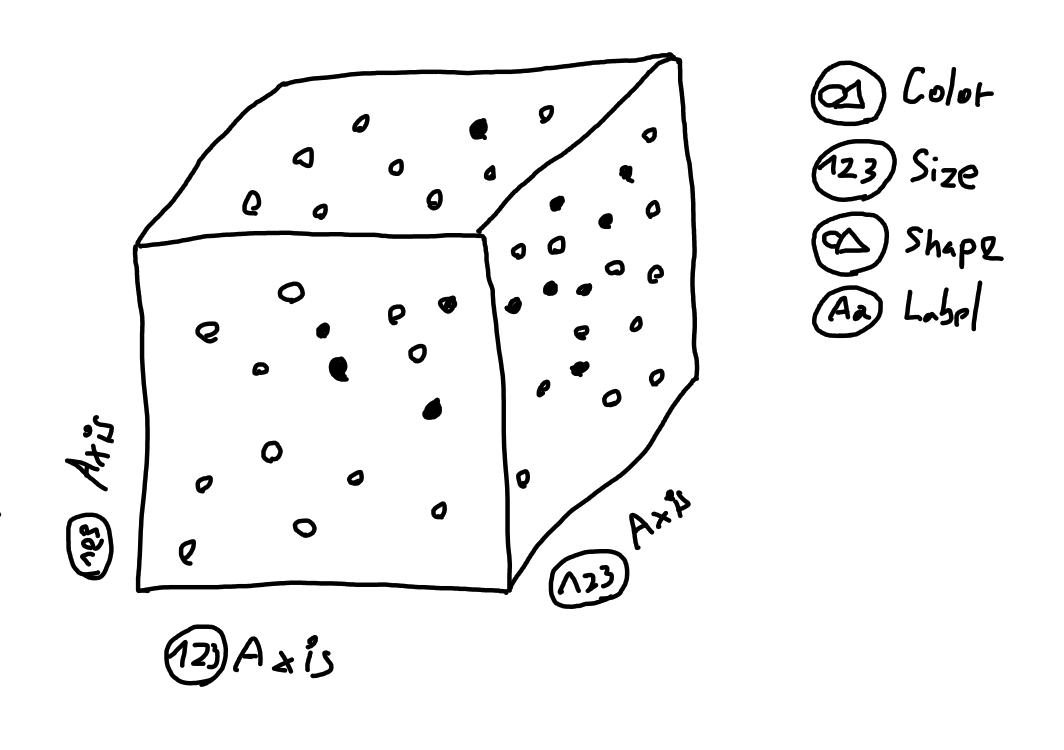
\includegraphics[scale=1]{sketch_plot}
\caption{Plot in VR.}
\label{fig:sketch_plot}
\end{figure}

The original design included a \emph{hot corners} feature, which enabled the user to physically grab corners of plot in 6DOF and stretch the plot by doing so. The August release substituted this feature for a more conventional resizing gesture. The faces of a plot's bounding box were to be used for setting bounds on spatial axes. Both features were replaced in the August build due to their reliance on room-scale --- the user was supposed to move around the room, which would make the experience uncomfortable. They were also incompatible with 3DOF input methods.

\begin{figure}[ht]
\centering
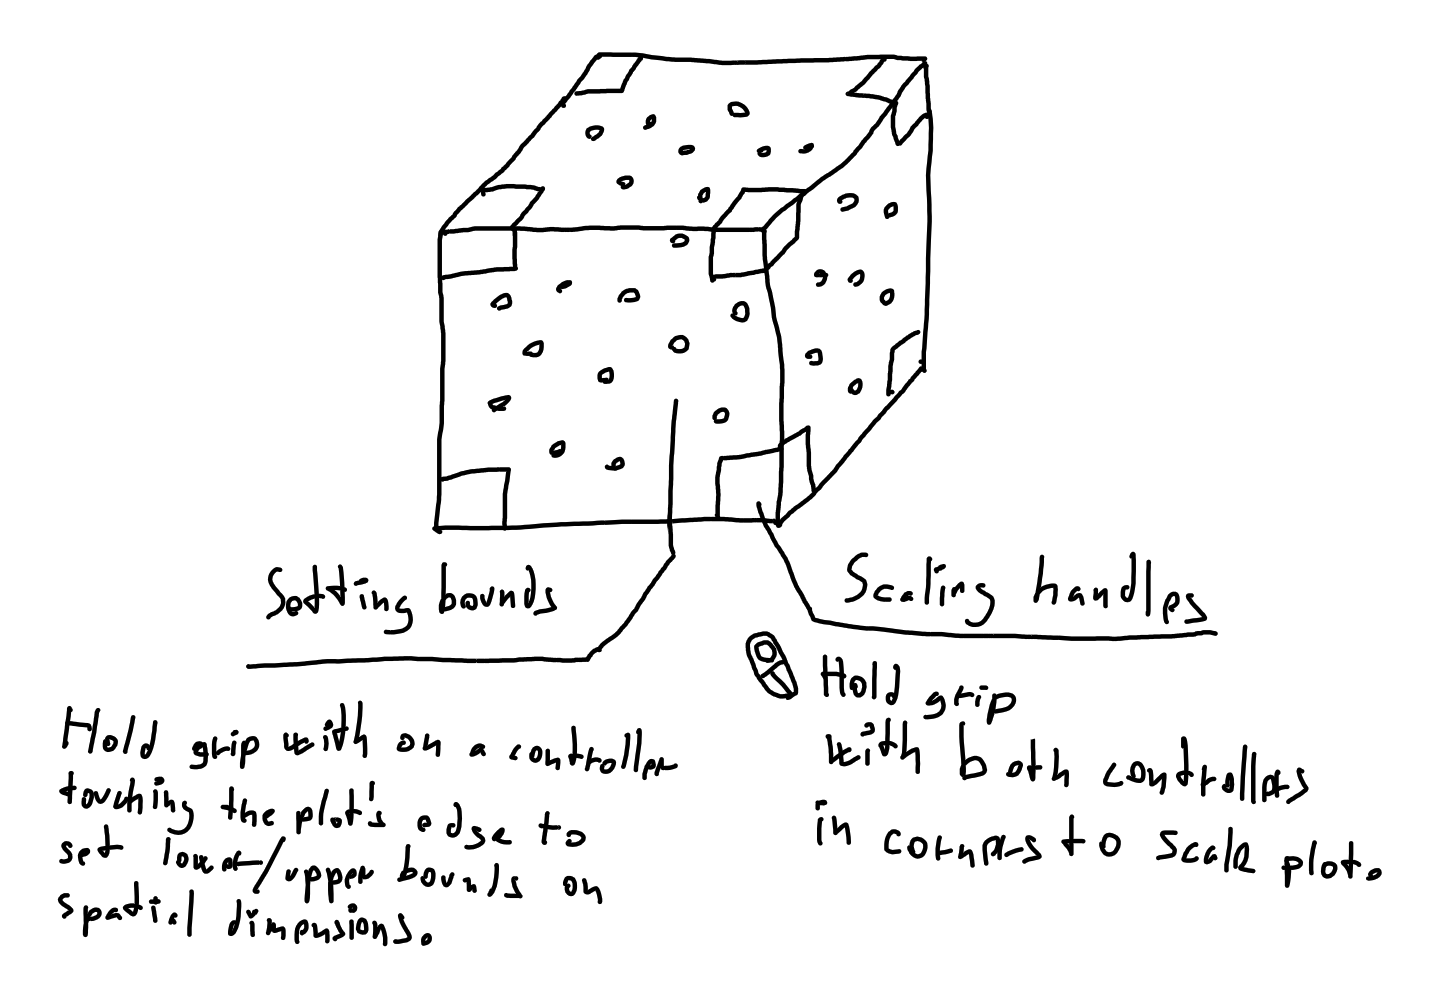
\includegraphics[scale=0.85]{sketch_6dofresize}
\caption{Plot resize interaction in 6DOF.}
\label{fig:sketch_6dofresize}
\end{figure}

The 6DOF version includes a panel attached to one of the controllers. This is possible due to the fact that 6DOF systems utilize two controllers --- the other controller can be used for dragging the attribute from the panel.

\begin{figure}[ht]
\centering
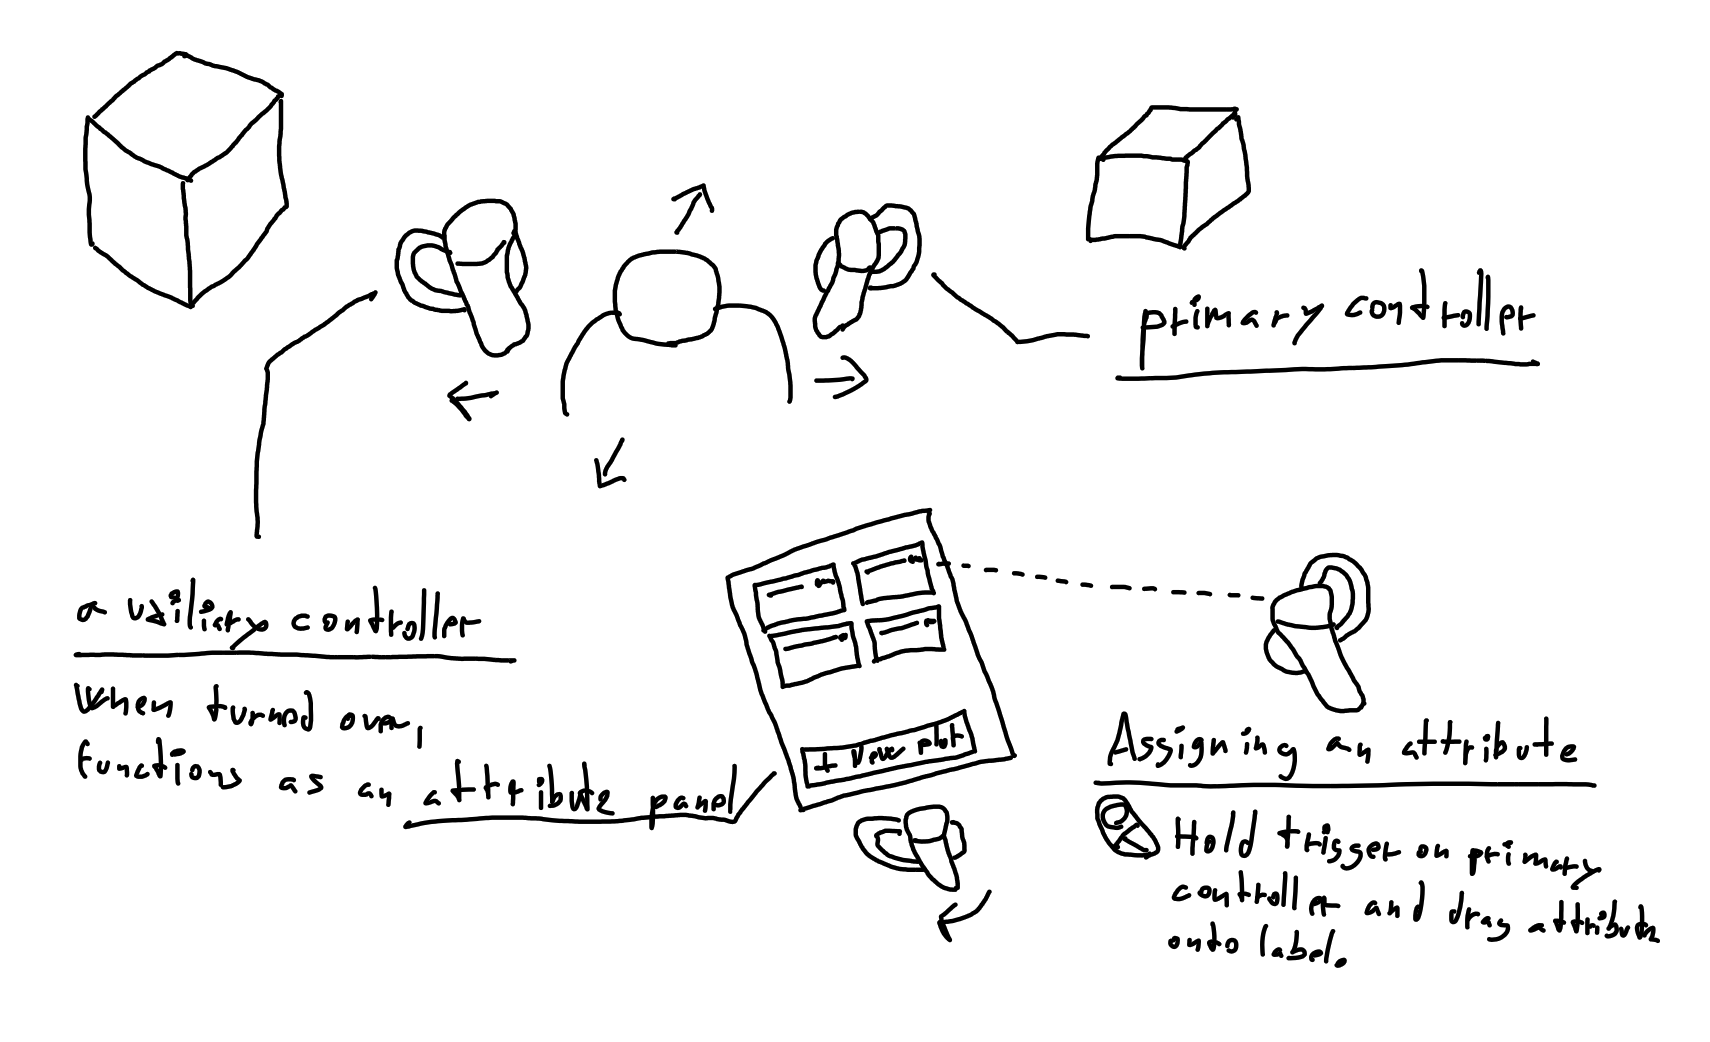
\includegraphics[scale=0.85]{sketch_6dofpanel}
\caption{Attribute assignment in 6DOF.}
\label{fig:sketch_6dofpanel}
\end{figure}

3DOF version offers no such luxury --- the panel is fixed in space. The plot can be moved along paths that resemble concentric rings and also pushed away from or towards the user. This design was subsequently used in both 3DOF and 6DOF, due to its comfort.

\begin{figure}[ht]
\centering
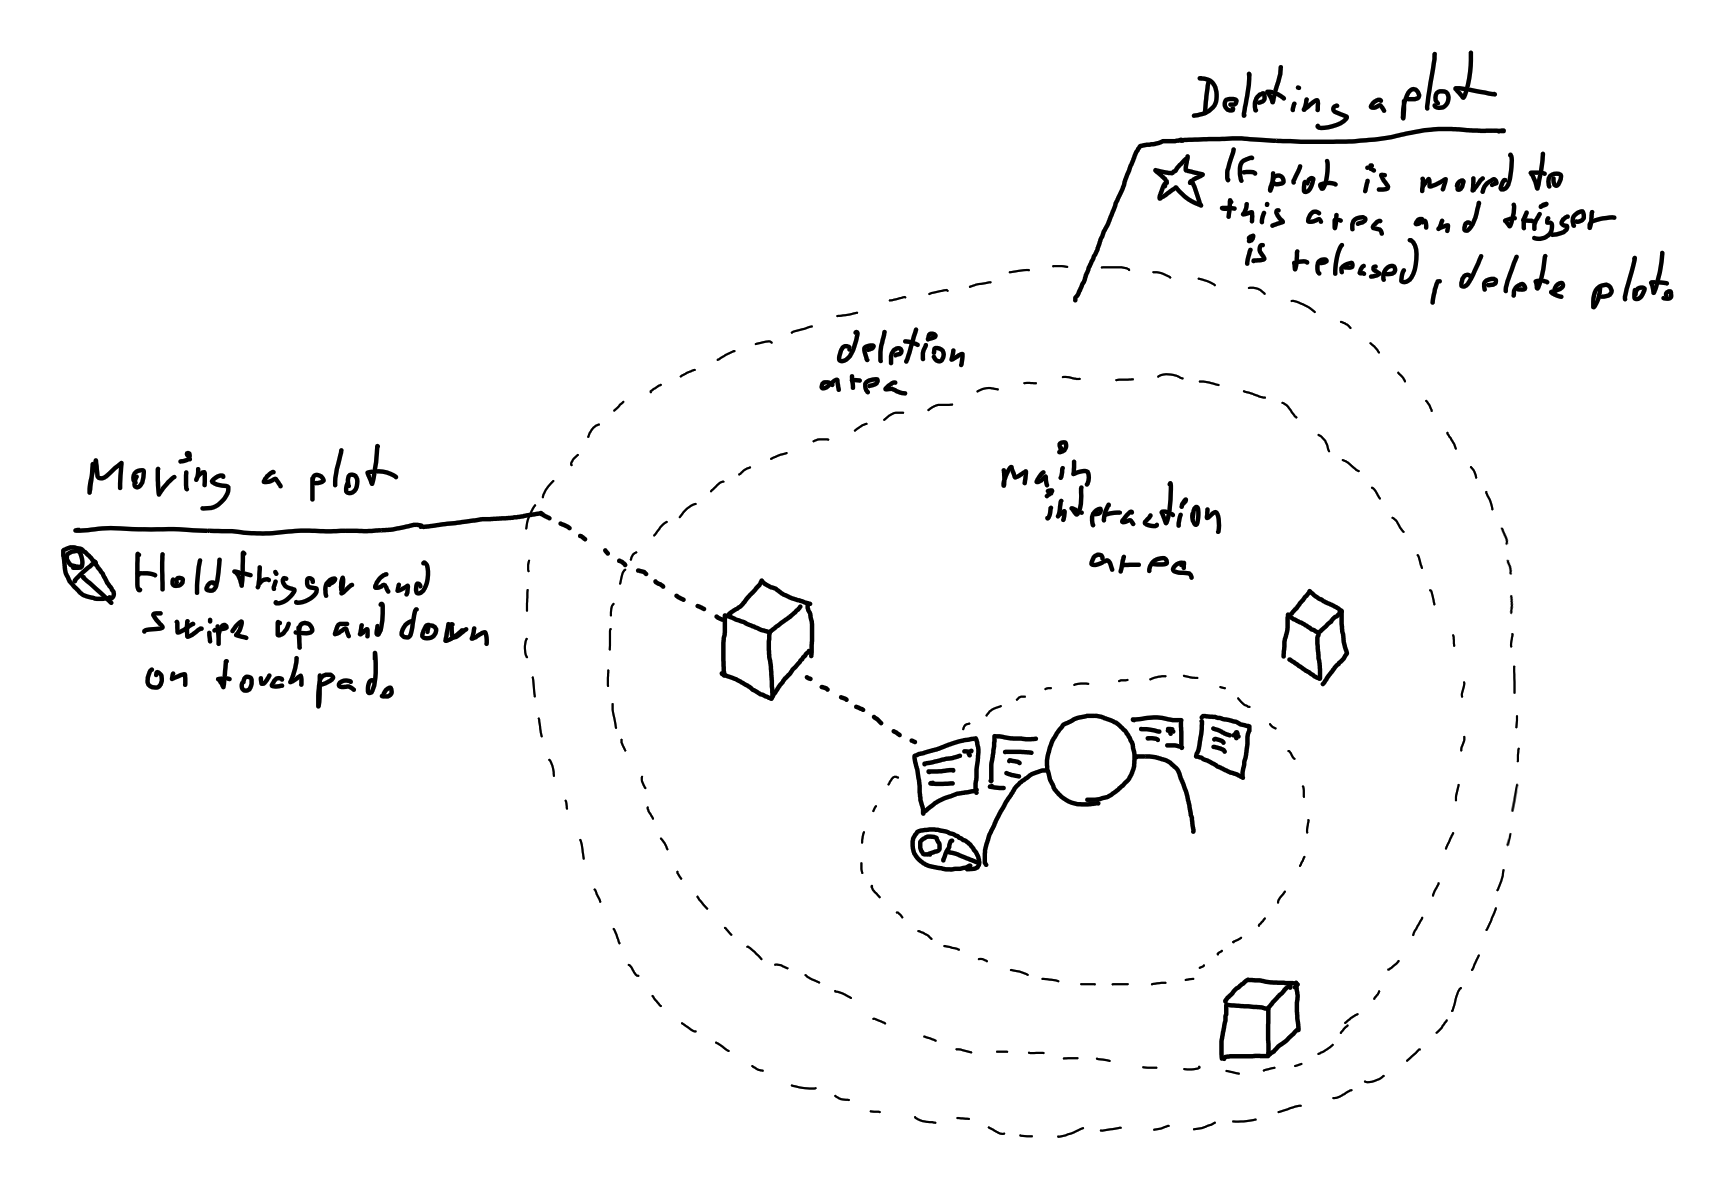
\includegraphics[scale=0.85]{sketch_3dofspace}
\caption{Spatial design of the 3DOF version.}
\label{fig:sketch_3dofspace}
\end{figure}

Another limitation of 3DOF headsets is their controller (provided there is any). The following sketch shows input options of an Oculus Go controller along with bindings for Navigator.

\begin{figure}[ht]
\centering
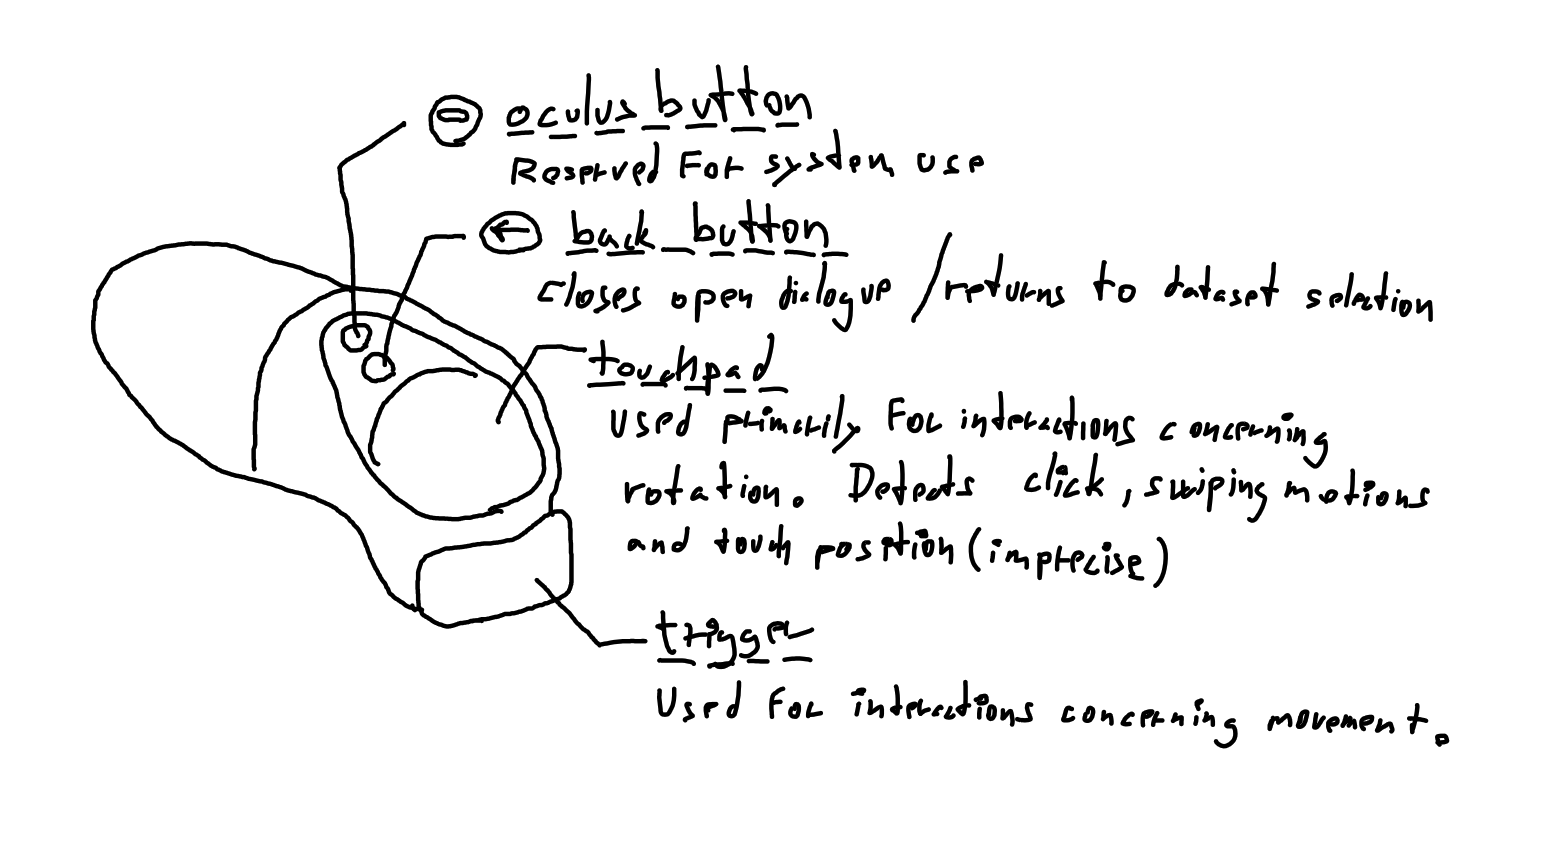
\includegraphics[scale=0.85]{sketch_3dofcontroller}
\caption{Input capabilities of an Oculus Go controller.}
\label{fig:sketch_3dofcontroller}
\end{figure}

\section{January build (1901)}

\begin{figure}[ht]
\centering
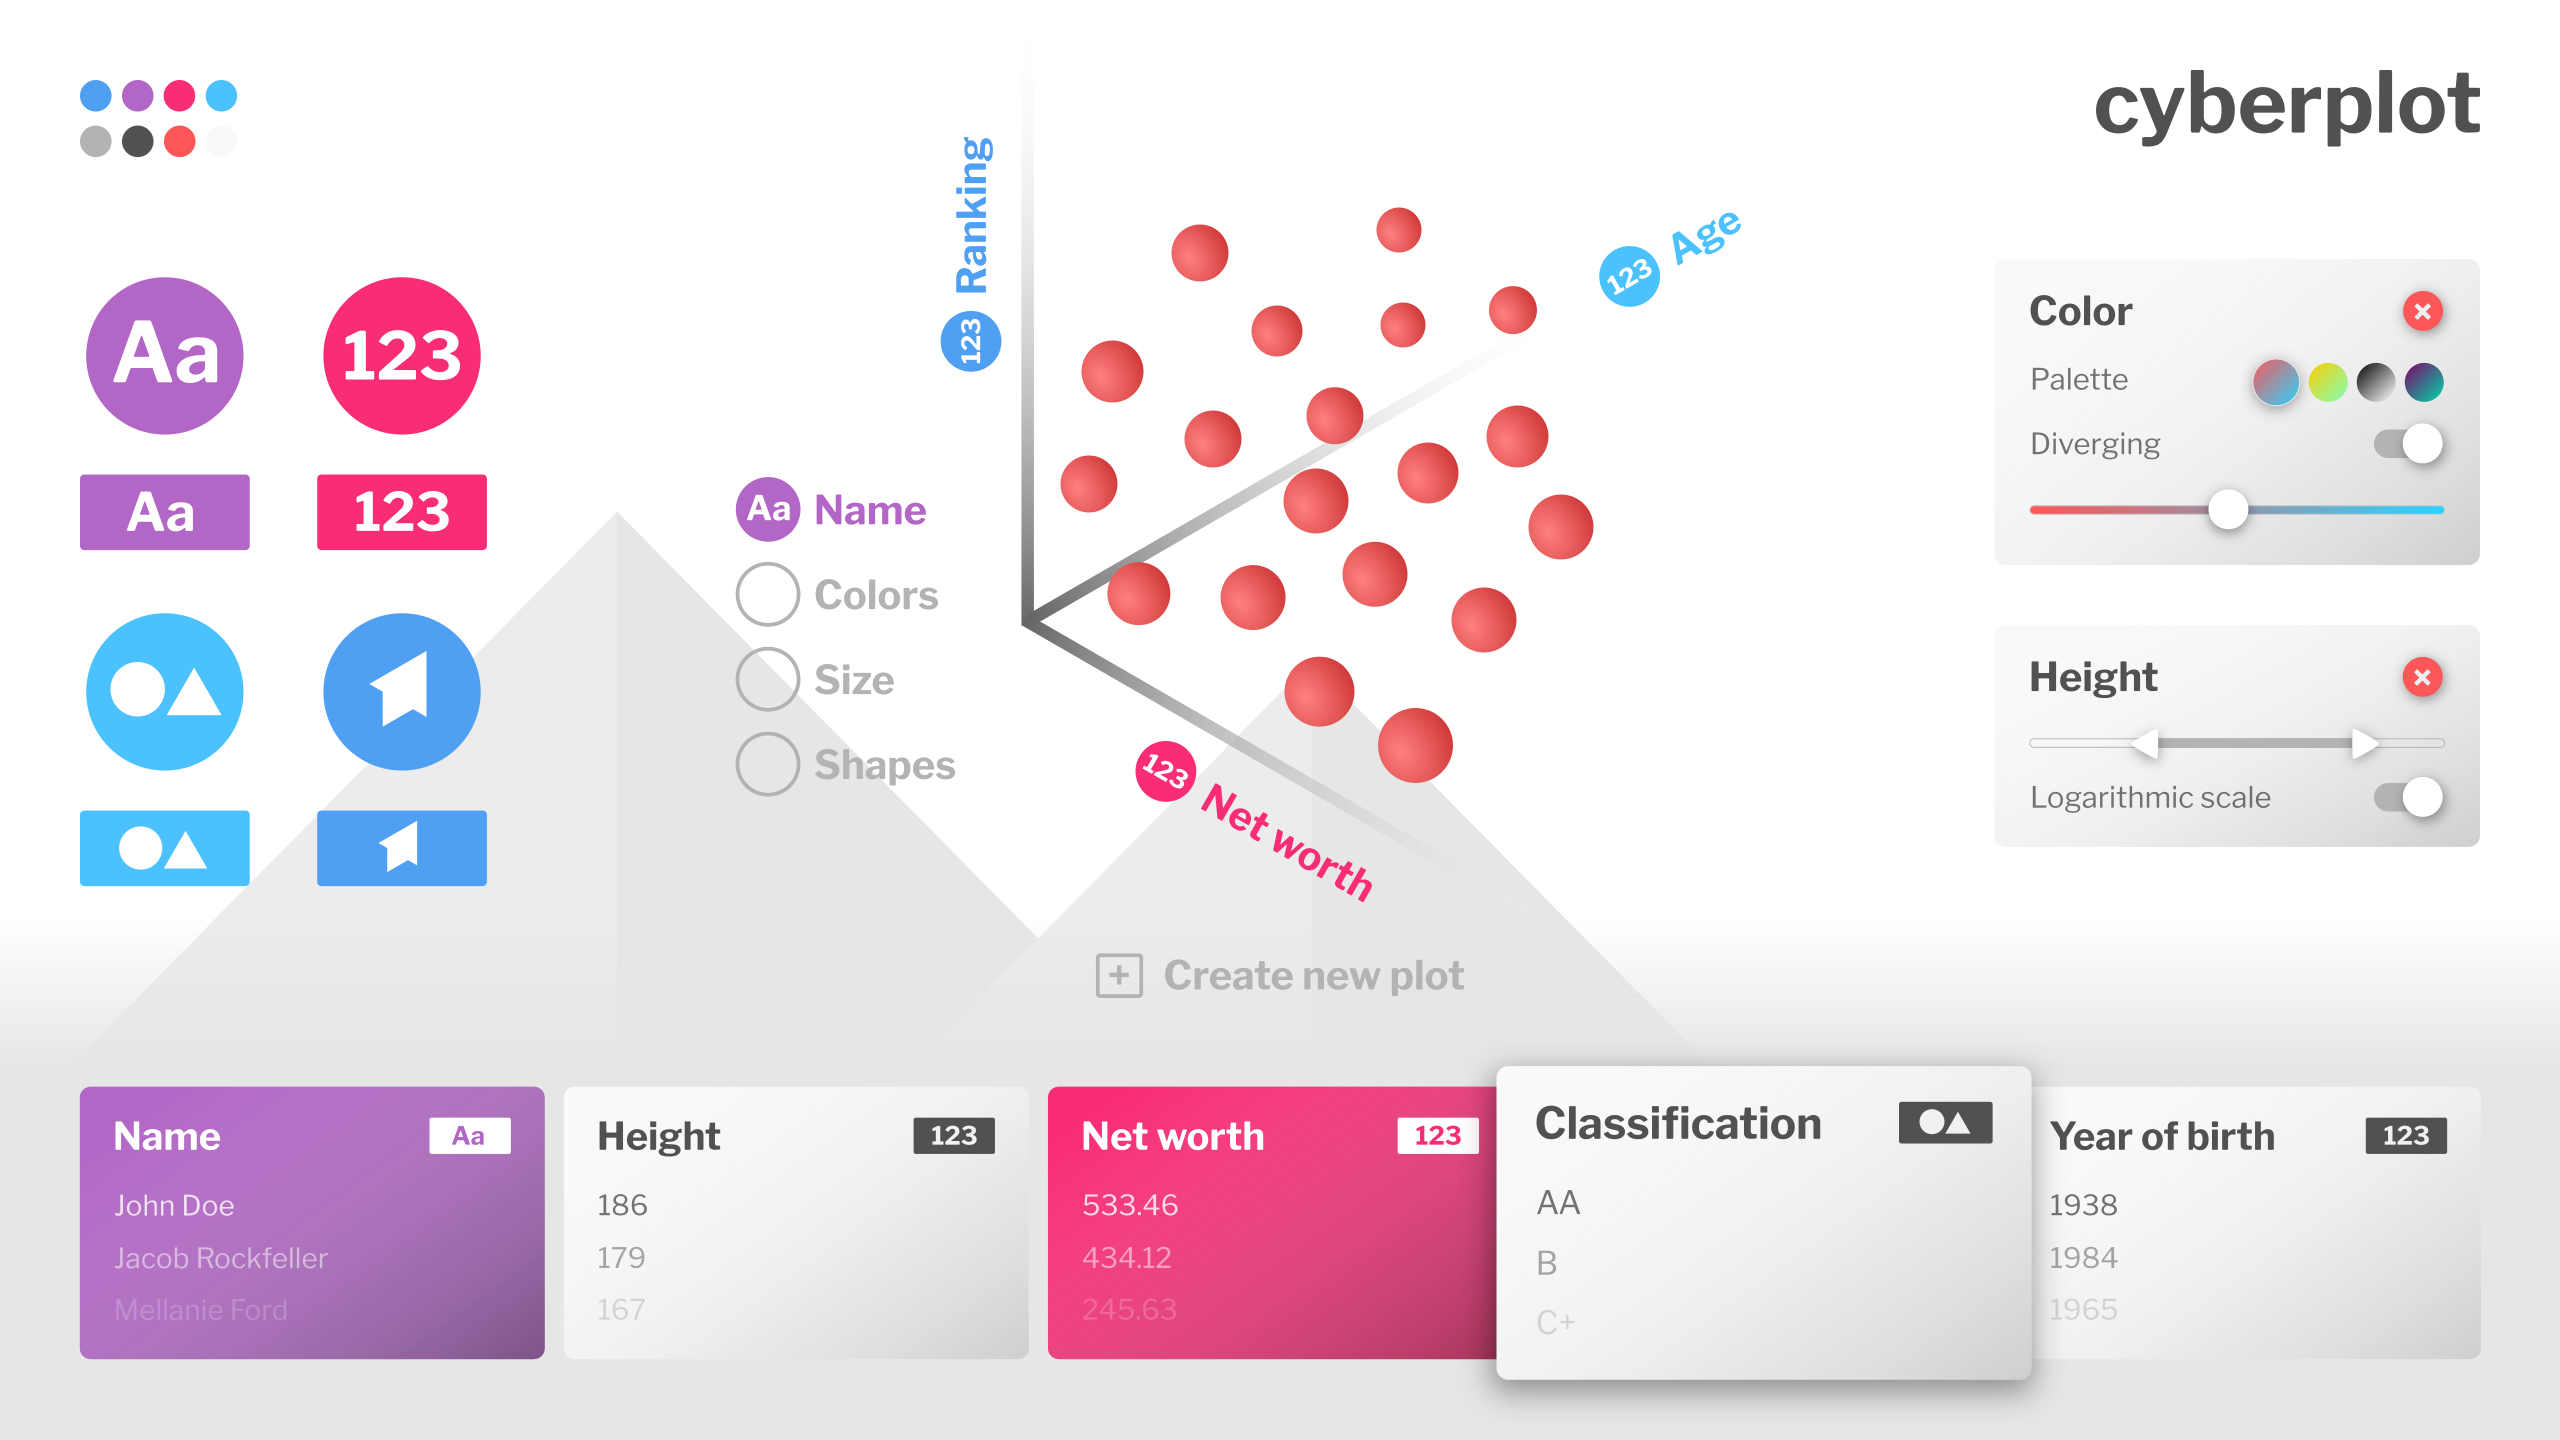
\includegraphics[scale=0.2]{ui_design}
\caption{Initial user interface design for Navigator.}
\label{fig:ui_design}
\end{figure}

The January build highlighted basic interactions in 3DOF. User interface design was influenced by Google's Material Design\autocite{materialdesign} and a tech demo called Daydream Elements.\autocite{daydreamelements} The user was able to select one of the preloaded datasets, create scatter plots, position them in space and assign attributes to them. The design of dataset panel remained unchanged in later revisions. Attributes are color-coded on assignment, which is useful when working with multiple plots. In this version, the user can assign attributes onto spatial axes of a plot as well as the color feature, however the functionality is still quite basic --- spatial axes only support numerical attributes, while the color feature only accepts categorical attributes. The background used a mixture of white and light gray and has been scrapped in future revisions due to the fact that it caused fatigue.

\begin{figure}[ht]
\centering
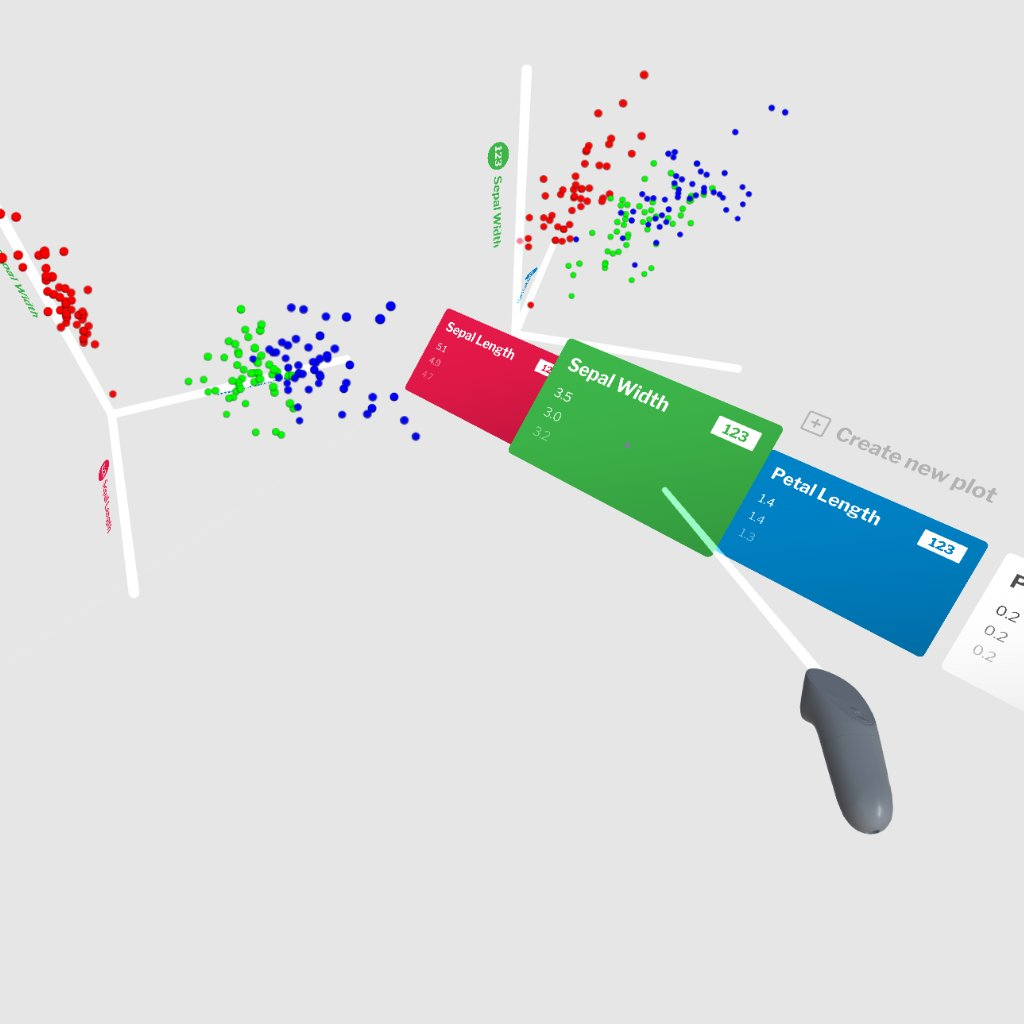
\includegraphics[scale=0.2]{navigator_1901}
\caption{Screenshot from the January build of Navigator.}
\label{fig:navigator_1901}
\end{figure}

\section{Lo-fi prototype}

The next stage of prototyping involved using Microsoft Maquette.\autocite{msmaquette} More detailed versions of panels discussed in the subchapter on interaction design were created, this time taking multiple datasets into account.

\begin{figure}[ht]
\centering
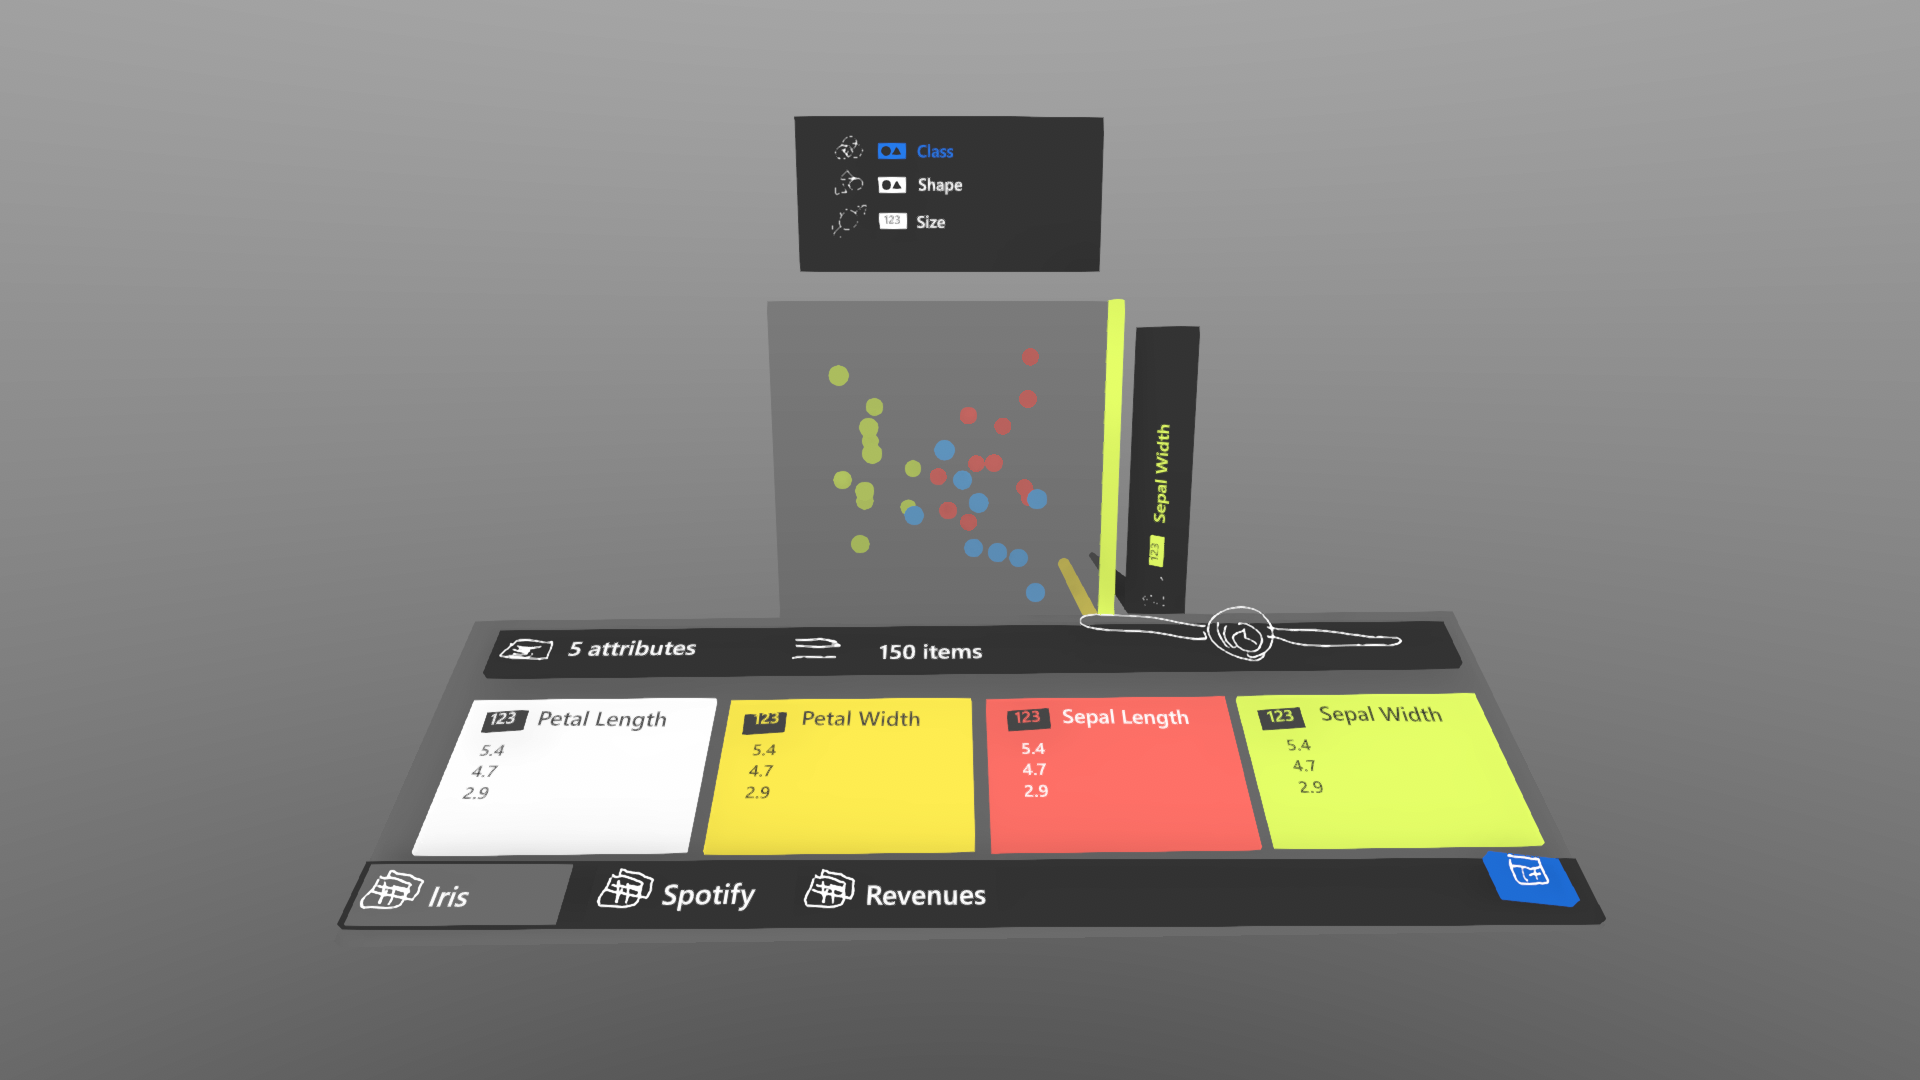
\includegraphics[scale=0.15]{maquette_databrush_3dof}
\caption{Prototype of 3DOF interface.}
\label{fig:maquette_databrush_3dof}
\end{figure}

New hierarchy was introduced around this time, alongside terminology like space and version. \emph{Space} is defined as an area in which visualization takes place. Inside the space, the user can interact with multiple \emph{datasets}, which can contain multiple versions. Attributes from datasets can be assigned to a number of \emph{plots}, which in turn display data from the currently selected 
\emph{version}.

\begin{figure}[ht]
\centering
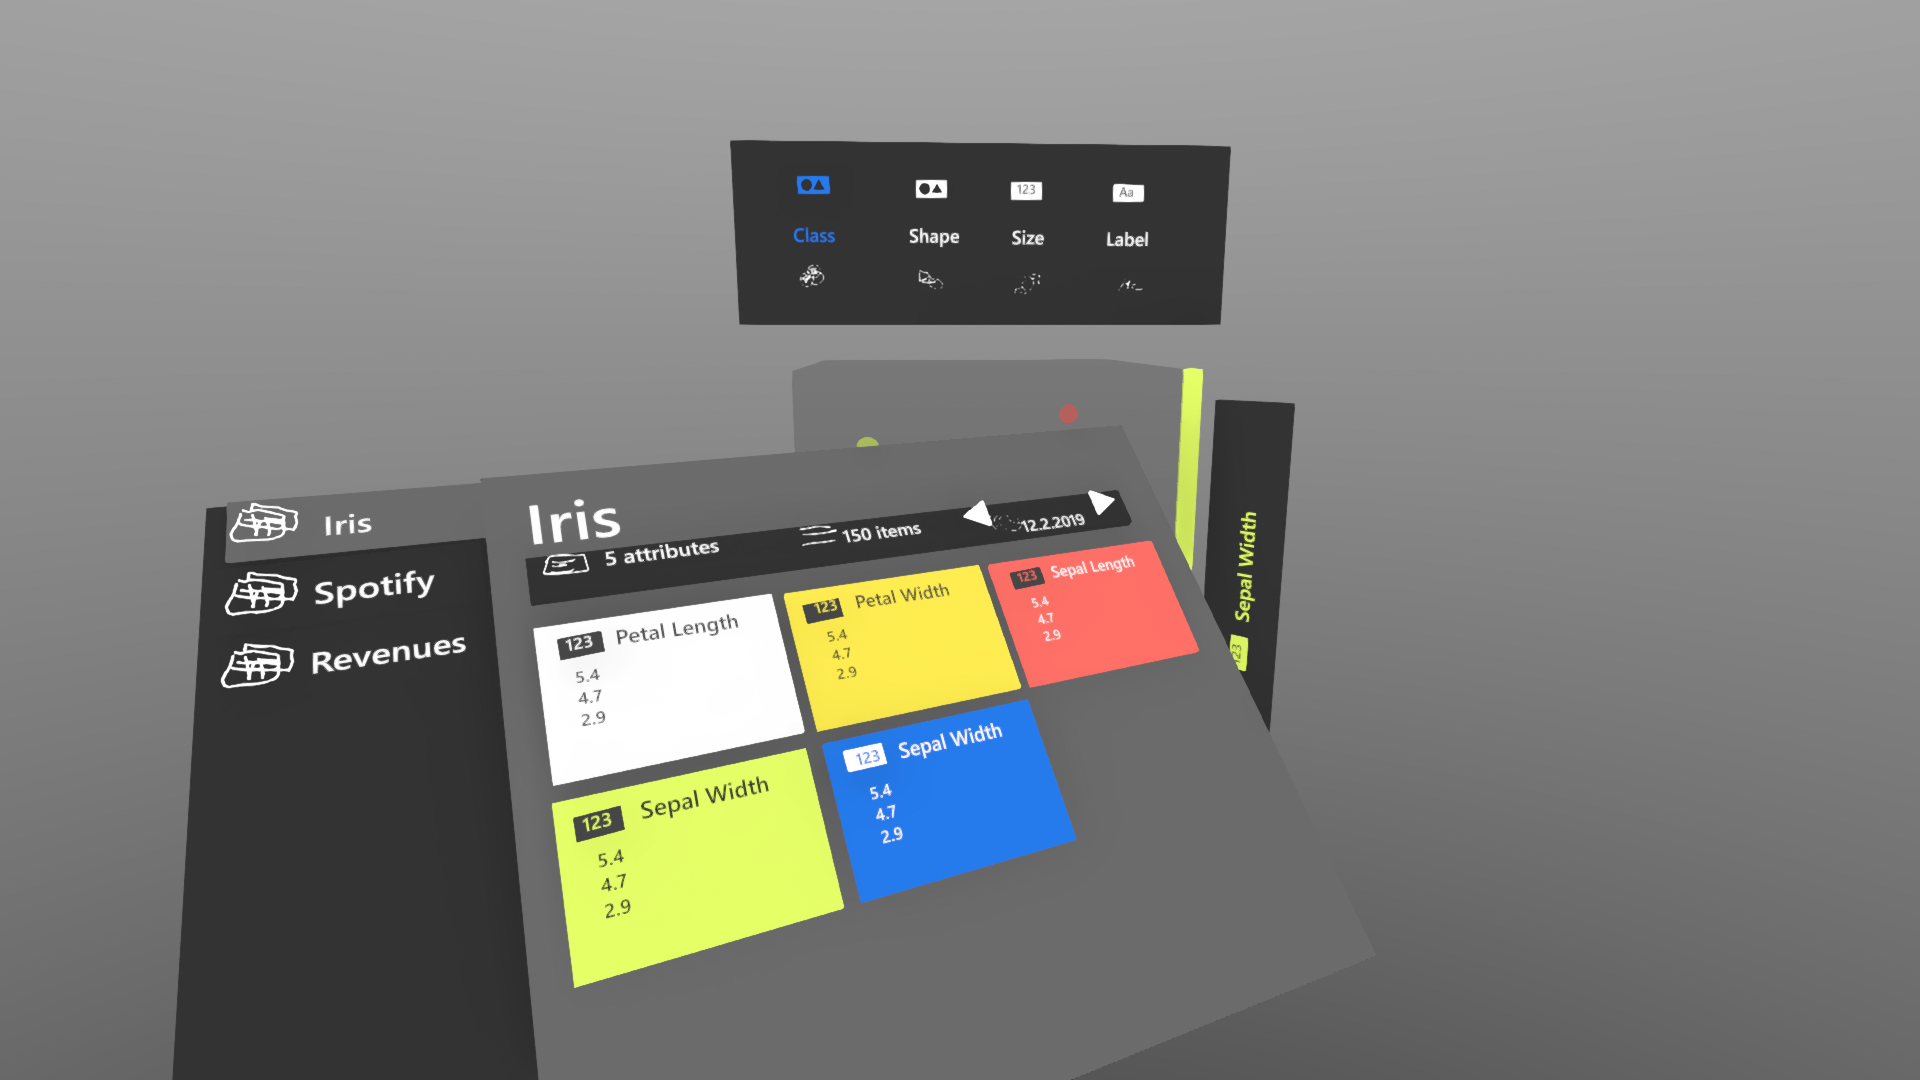
\includegraphics[scale=0.15]{maquette_databrush_6dof}
\caption{Prototype of 6DOF interface highlighting the 6DOF data brush.}
\label{fig:maquette_databrush_6dof}
\end{figure}

\section{August build (1908)}

The August build of Navigator added integration with Manager. When the user first launches Navigator on their VR headset, they are presented with a 5-digit numeric code, which is used for pairing their account. This system was chosen in order to mitigate poor text input capabilities in virtual reality.

\begin{figure}[ht]
\centering
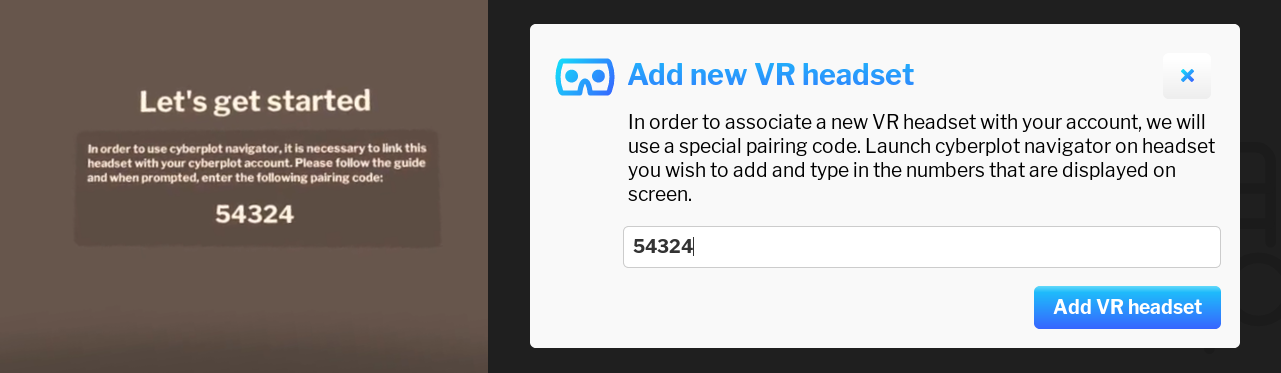
\includegraphics[scale=0.2]{pairing}
\caption{Left: Pairing prompt in Navigator. Right: Adding a new headset in Manager.}
\label{fig:pairing}
\end{figure}

After logging in, the user can select one of their datasets, which is then loaded onto what we call a \emph{data brush}, essentially a simplified version of Manager's dataset view. In the 3DOF version, the data brush is present in a fixed position in front of the user's pelvis and while its visibility can be toggled, it is visible for the most part. In the 6DOF version, the user can display the data brush by holding down the grip button. It is then displayed on top of one of their controllers. The data brush displays dataset metadata and attribute listings, which look similar to their Manager counterpart. In order to reduce the amount of text and provide more information, we have opted to display histograms in place of data preview for numerical attributes. The user can move between pages of attributes by utilizing a flick gesture using their controller's analog stick or touchpad. They are also able to switch between versions if versioning is on for selected dataset and load additional datasets. The users are able to have multiple datasets open at the same time.

\begin{figure}[ht]
\centering
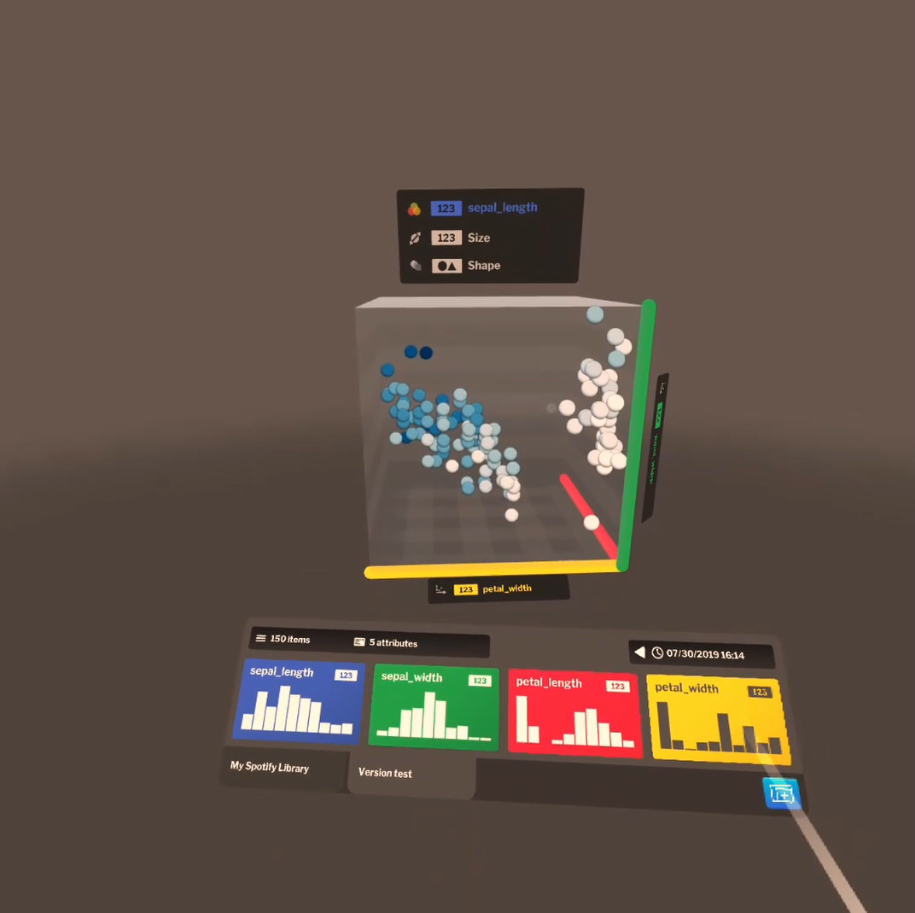
\includegraphics[scale=0.2]{cyberplot_3dof}
\caption{Navigator's 3DOF interface.}
\label{fig:cyberplot_3dof}
\end{figure}

Plots can be created by pointing at the floor and holding the trigger, which opens up a pie menu with available plot types. Selection can be made by moving the pointer onto an icon and releasing the trigger. This interaction enables the user to quickly create a plot anywhere inside the virtual environment. Plots can be moved around the user's current position by using the trigger and brought closer or further away by using the analog stick or joystick in conjunction with the trigger. If the user drags the plot far away, it turns red and, should the user release the trigger, is deleted from the scene.

Plots can also be rotated 90 degrees by pointing at them and using the aforementioned flick gesture. In 3DOF, we try to mitigate the lack of positional movement (which further enhances spatial perception) by offering a free-form rotation mode, which is triggered by pointing at the plot and pressing down on the touchpad. Doing so maps the rotation of a controller onto the rotation of the plot.

The plot can also be scaled, although the mechanics differ depending on VR system used. In 6DOF, one can scale a plot by pointing at it with both controllers, pressing the trigger and dragging inwards or outwards, a fairly standard gesture in VR interface design. In 3DOF we are unable to use this gesture, as most 3DOF systems come with only one controller. We have instead chosen to utilize a twisting motion, where the user twists their wrist in order to control the plot's scale. Such interaction technique had been previously implemented in the VR game \emph{Virtual Virtual Reality}.\autocite{vvr}

\begin{figure}[ht]
\centering
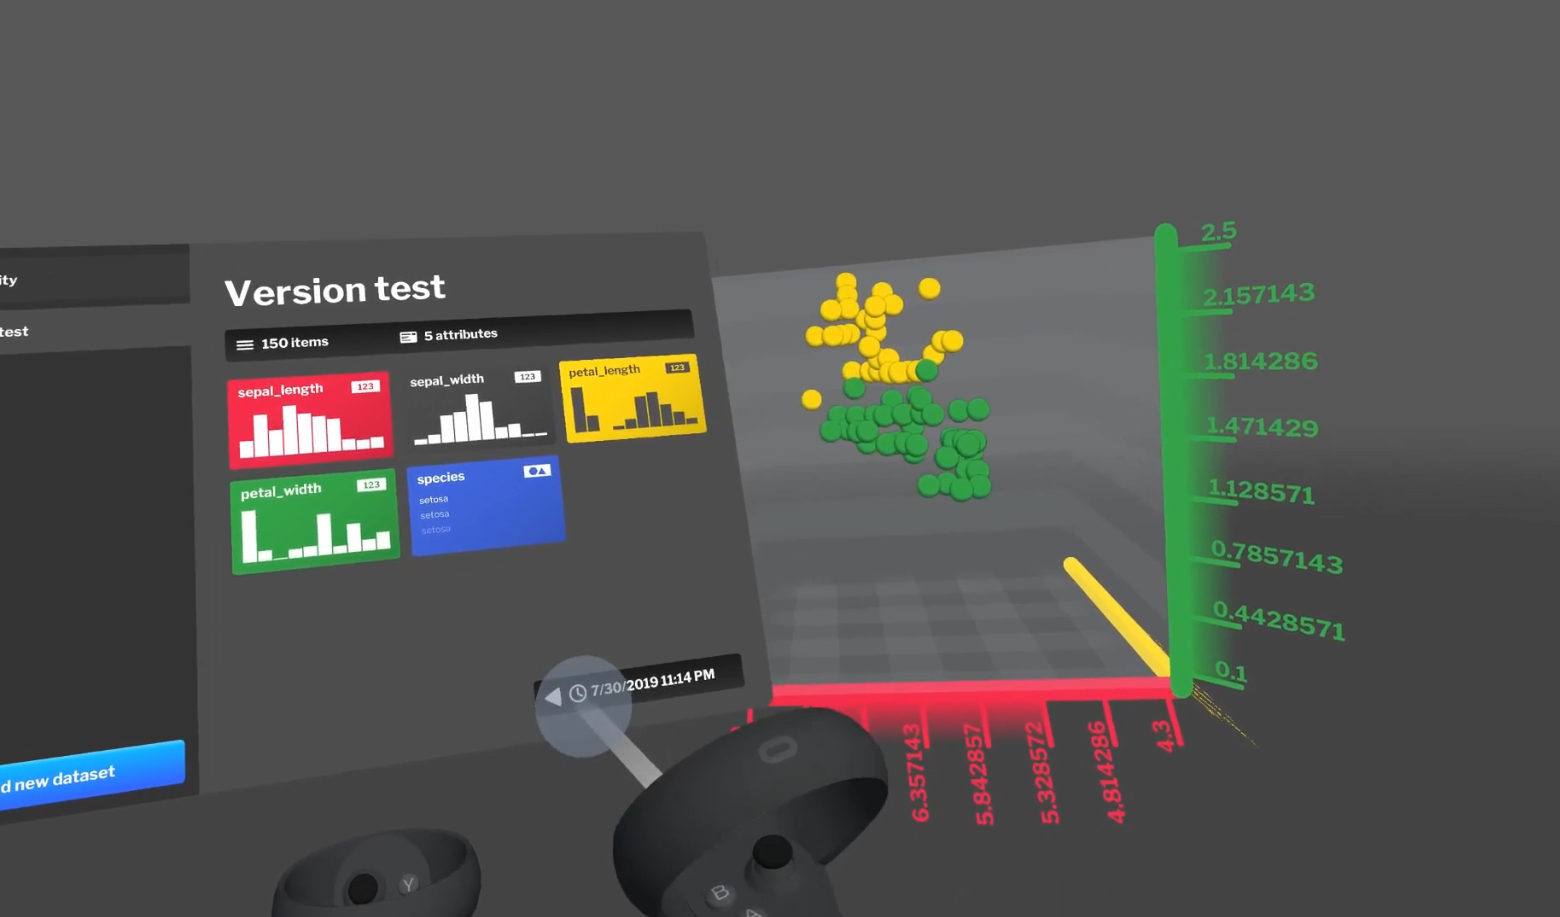
\includegraphics[scale=0.2]{cyberplot_6dof}
\caption{Navigator's 6DOF interface.}
\label{fig:cyberplot_6dof}
\end{figure}

Attributes can be dragged from the data brush onto individual plots by using the trigger button. In the case of scatter plots, they can be assigned to spatial axes and non-spatial features like color and size. When we assign an attribute onto spatial axes, the position of nodes is smoothly interpolated to their new position in order to provide a visual cue to the user. Once an attribute is assigned, it is color-coded on both the plot and the data brush. Color-coding persists until the attribute in question is removed from all plots. Assignments can be reversed by using the trigger button.

Scatter plots also display scales. For numerical attributes we display numerical values for a set number of steps, for categorical attributes, steps are made for each value. The user is able to slice the plot by creating bounds. These are created by pressing on a desired position on a scale.

\section{Lo-fi prototype #2}

The next iteration of prototyping revolved around work on immersive mode, statistics panel, collaboration features and a filtering interface.

Immersive mode is a feature that enables the user to physically enter one of the plots. In addition to enabling the user to immerse themselves in a subset of data, it also allows us to do some technical optimization, an example of which is rendering glyphs in scatter plots. When immersive mode is inactive, all glyphs are rendered as billboarded sprites. Upon entering immersive mode, they change into 3D meshes, which is a necessity given they can move much closer to the user.

\begin{figure}[ht]
\centering
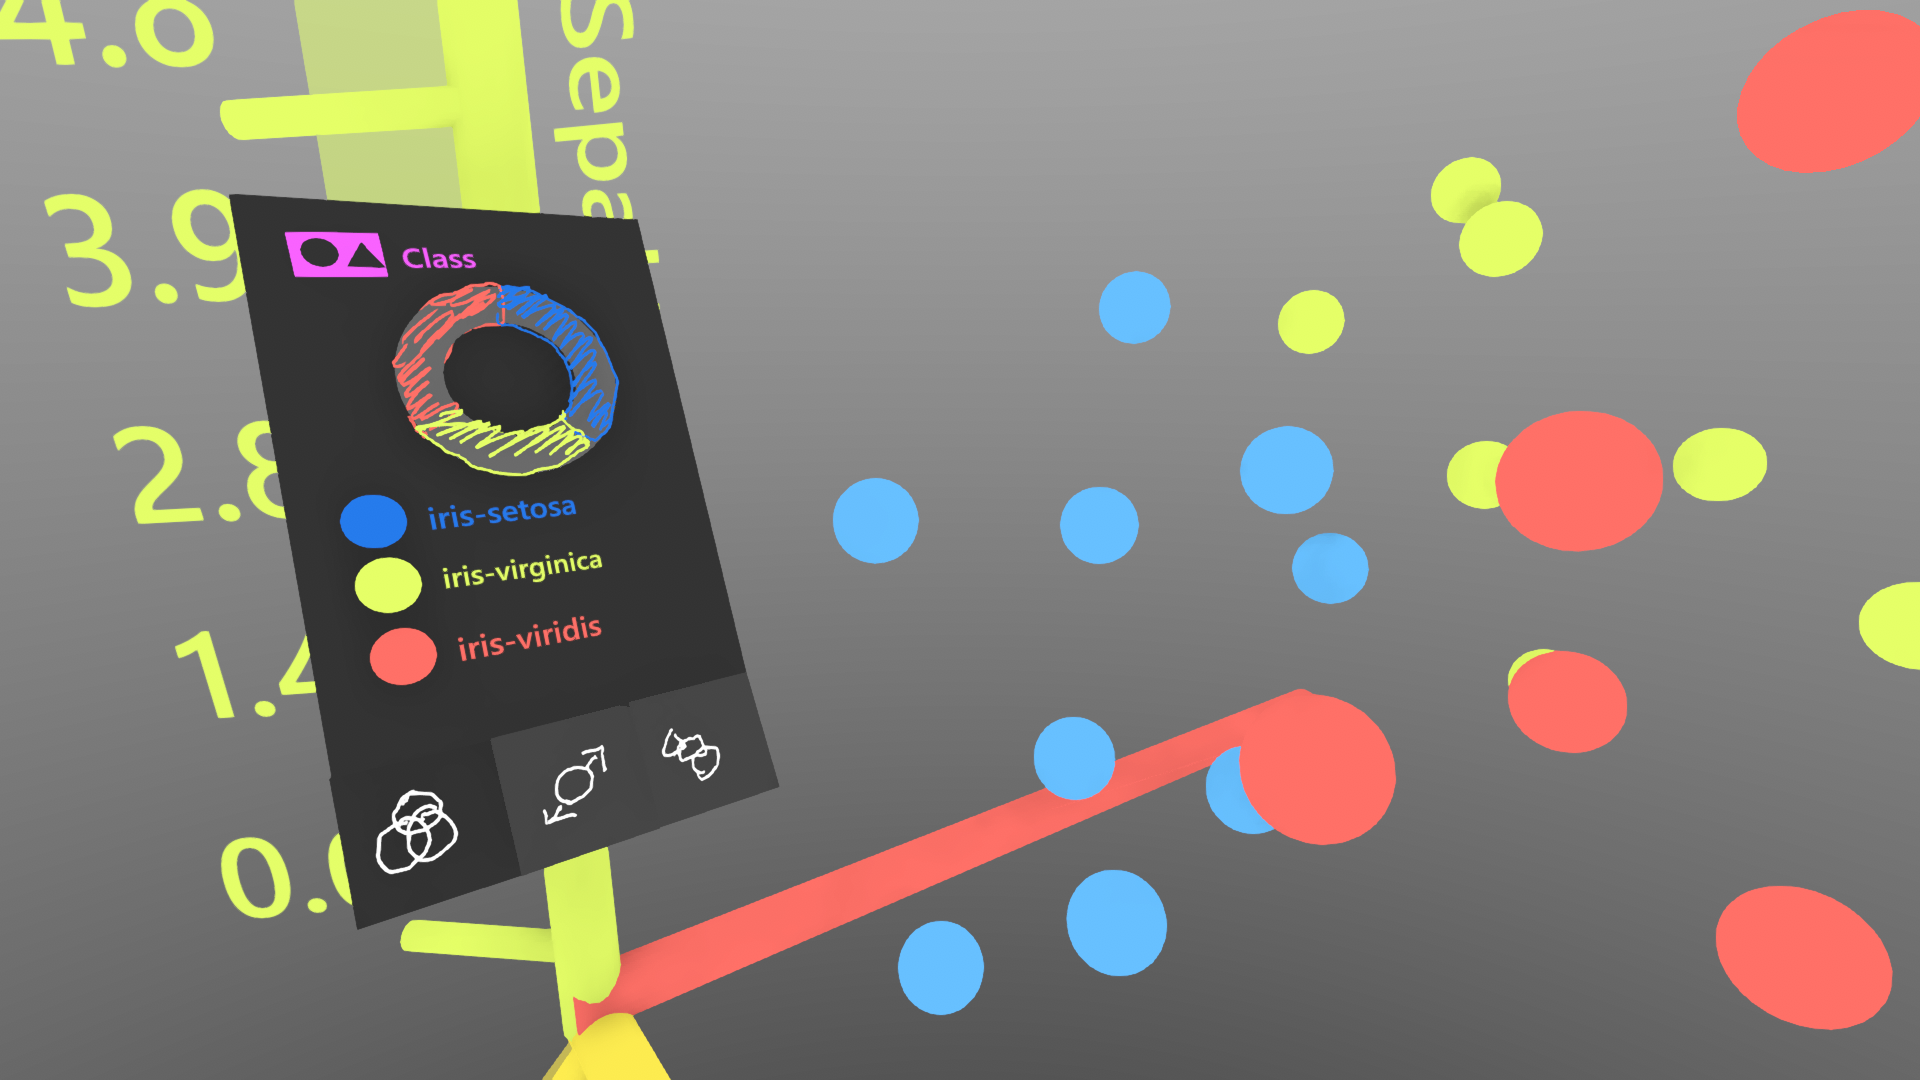
\includegraphics[scale=0.15]{maquette_statistics}
\caption{Prototype of the immersive mode.}
\label{fig:maquette_statistics}
\end{figure}

When the user enters immersive mode, they have the option of displaying statistics for non-spatial features of the plot. These are displayed on a panel above the controller.

\begin{figure}[ht]
\centering
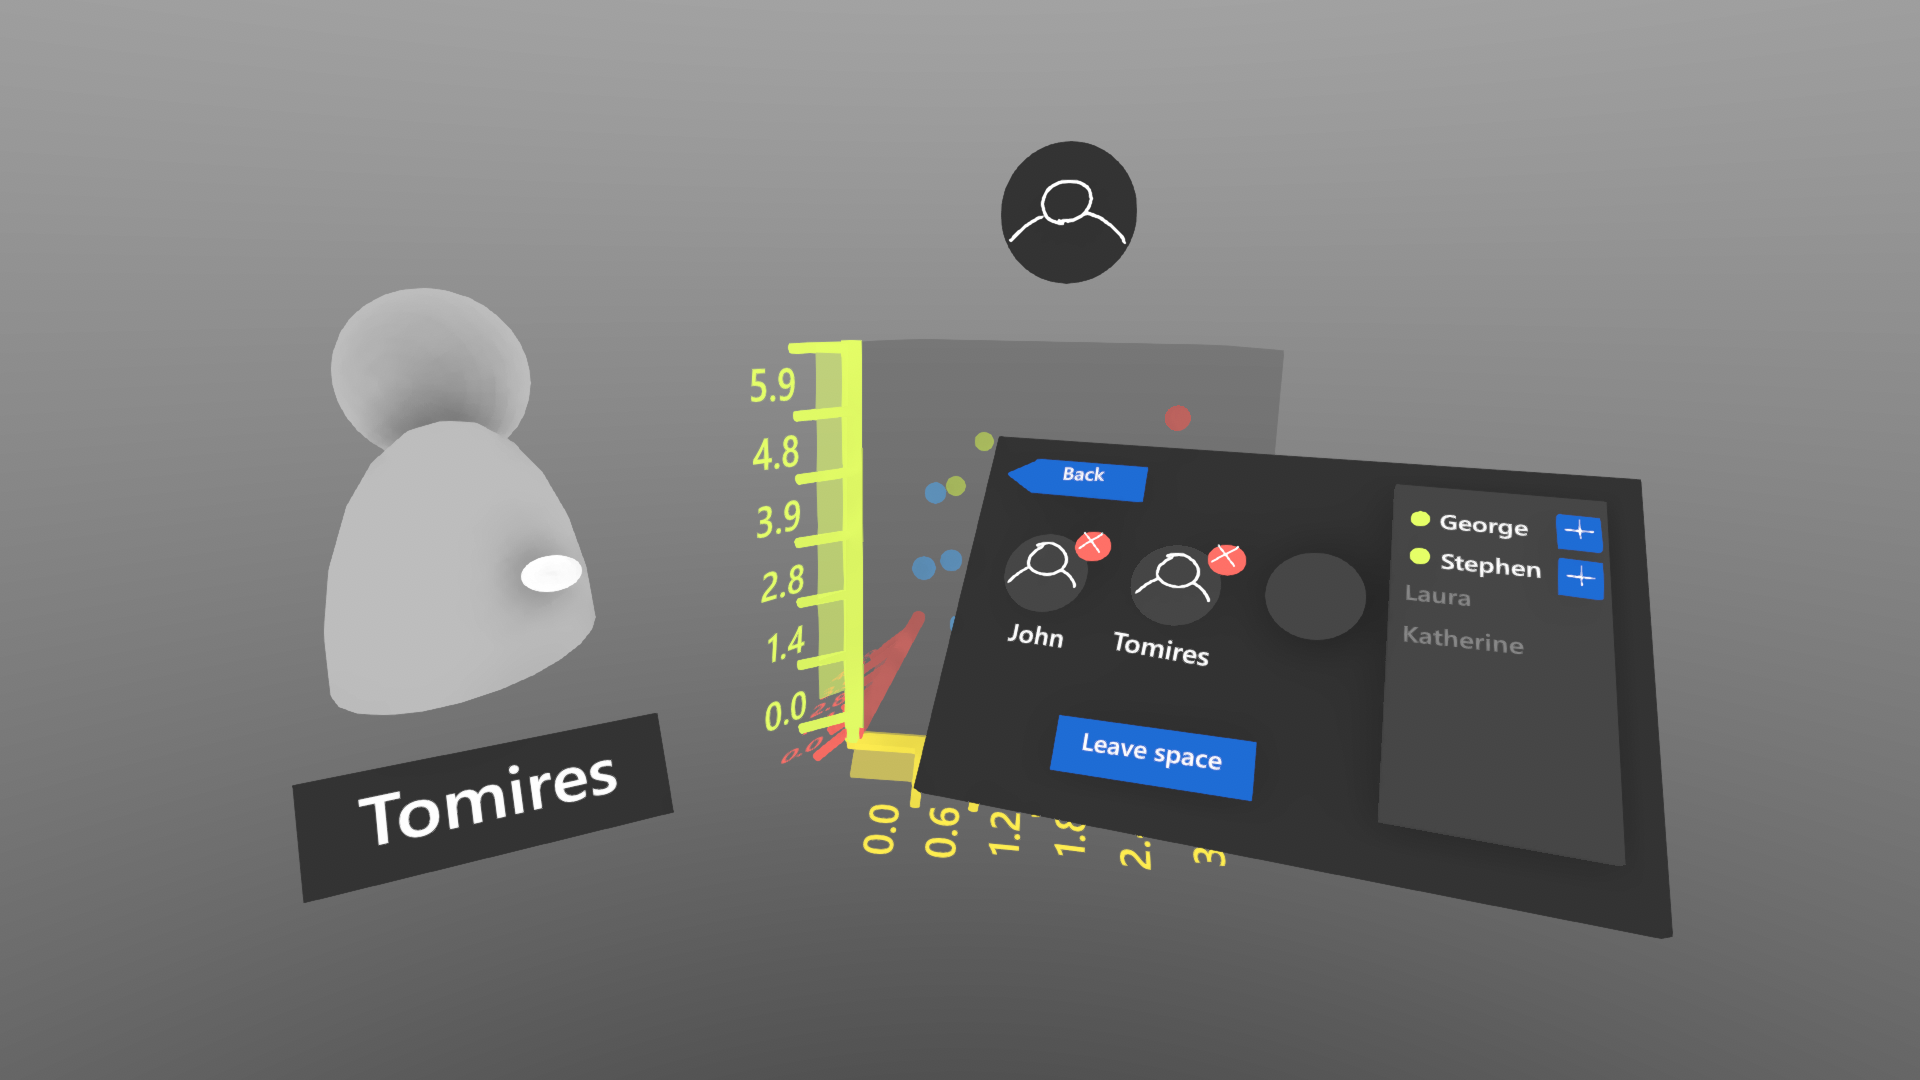
\includegraphics[scale=0.15]{maquette_collaboration}
\caption{Prototype of collaboration with two other users, one of which is inside immersive mode.}
\label{fig:maquette_collaboration}
\end{figure}

Collaborative features allow the user to invite their colleagues from within the data brush. They can also see their avatars along their sides or, in the case of immersive mode, anywhere inside the plot. Body, head and controller positions are tracked and transmitted over the network, allowing for the utilization of pointing gestures. Voice communication is also enabled.

\begin{figure}[ht]
\centering
\includegraphics[scale=0.15]{maquette_filtering}
\caption{Prototype of the filtering interface.}
\label{fig:maquette_filtering}
\end{figure}

The last feature that we have prototyped is a plot-specific filtering system. It enables the user to select any numerical attribute from the current dataset and change the range of displayed values. This is an extension of the existing \emph{slicing} mechanic present in scatter plots.

\section{December build (1912)}

The December build introduced a variety of new functionality, most notably immersion mode and multiple plot types. Several changes were also made to existing UI elements based on feedback.

\begin{figure}[ht]
\centering
\includegraphics[scale=0.12]{navigator_plottypes}
\caption{Plot types available to the user.}
\label{fig:navigator_plottypes}
\end{figure}

Users now have the ability to choose from 5 distinct plot types. These are selectable from a redesigned pie menu, which features new iconography. Two new attribute types debut in Navigator with the introduction of locational and spatial attributes. The former can be used with globe and map plots, while the latter can be assigned onto box and surface plots.

\begin{figure}[ht]
\centering
\includegraphics[scale=0.4]{navigator_plotselector}
\caption{Pie menu used for selecting the type of a newly created plot.}
\label{fig:navigator_plotselector}
\end{figure}

Free-form rotation mode from the previous version was replaced by the all-new immersive mode. Inside immersive mode, the user can move freely in three dimensions by pointing their controller in a certain direction and pulling on the analog stick or by using the touchpad. A grid is displayed in the background as the user moves around the space in order to reduce the risk of motion sickness. This technique was borrowed from Google Earth VR.\autocite{earthux} As mentioned previously, a statistics panel, dubbed the \emph{Swatch} can be displayed at the user's convenience.

\begin{figure}[ht]
\centering
\includegraphics[scale=0.35]{statistics}
\caption{Screenshot of Navigator highlighting immersive mode. Swatch is visible on the left.}
\label{fig:statistics}
\end{figure}

The motivation for creating the statistics panel was a need to show context for non-spatial features of a plot. The initial design had the user flick their wrist akin to looking at a wristwatch in order to reveal the interface. Later revisions reused the same panel that is used for the data brush.

\begin{figure}[ht]
\centering
\includegraphics[scale=0.075]{statistics_original}
\caption{Unused, alternative layout for statistics.}
\label{fig:statistics_original}
\end{figure}

The final design contains a smaller panel which allows the user to toggle between different non-spatial features of the graph. The layout changes depending on assigned attribute.

\begin{figure}[ht]
\centering
\includegraphics[scale=0.075]{statistics_color}
\caption{Swatches for the plot's color feature.}
\label{fig:statistics_color}
\end{figure}

If a categorical attribute is assigned to the color feature, a pie chart is displayed. A gradient alongside quartiles is displayed for numerical attributes. Mapping onto quartiles is used as a compromise, as suggested by an article found online.\autocite{colormapping}

\begin{figure}[ht]
\centering
\includegraphics[scale=0.075]{statistics_size}
\caption{Swatches for the plot's size feature.}
\label{fig:statistics_size}
\end{figure}

The size feature in scatter plots only allows for assignment of numerical attributes. Quartiles are displayed.

\begin{figure}[ht]
\centering
\includegraphics[scale=0.05]{statistics_shape}
\caption{Swatches for the plot's shape feature.}
\label{fig:statistics_shape}
\end{figure}

When mapping a numerical attribute onto the shape feature, the values are divided into two bins of equal or similar size based on the median value. Each bin is then assigned a shape. If the attribute in question is categorical, unique values are mapped onto three distinct shapes. If more than three unique values exist, one of the shapes is used for multiple values.

\chapter{Testing}

In this chapter, we will compare the efficiency of our application against that of its contemporary alternatives introduced in the first chapter, introduce our testing methodology and present some of the findings.

\section{Example task}

The following table lists all KLM operations necessary to complete the task of creating a three-dimensional scatter plot as outlined in the second chapter. It presumes we are logged into Manager and have already associated a VR headset with our account.

\begin{table}[!h]
\centering
\caption{Listing of KLM operations for Cyberplot.}
\label{klm-cyberplot}
\scalebox{0.6}{
\begin{tabular}{lll}
Operator & Description & Time (s)\\
M & Initiate opening a file & 1.35\\
M & Find \emph{Add new dataset} button on sidebar & 1.35\\
PB & Point at the button and press it & 1.3\\
PB & Select \emph{Local file} & 1.3\\
PB & Click on \emph{Next} & 1.3\\
PB & Click on \emph{Select file} & 1.3\\
PB & Select file and double click it & 1.3\\
PB & Click on \emph{Next} & 1.3\\
M & Put on the VR headset with Navigator running & 1.35\\
B & Display the data brush by holding the grip button  & 0.2\textsuperscript{6DOF}\\
PB & Point on a dataset and press the trigger & 1.3\\
B & Hide the data brush by releasing the grip button & 0.2\textsuperscript{6DOF}\\
PBPB & Point on the ground, hold trigger, select scatter plot icon, release the trigger & 2.6\\
B & Display the data brush by holding the grip button & 0.2\textsuperscript{6DOF}\\
M & Locate the data brush & 1.35\textsuperscript{3DOF}\\
2*(PBPB) & Drag attributes onto two of the spatial dimensions & 5.2\\
PB & Rotate the plot & 1.3\\
PBPB & Drag an attribute onto the remaining spatial dimension & 2.6\\
PBPB & Drag an attribute onto the color dimension & 2.6\\
B & Hide the data brush by releasing the grip button & 0.2\textsuperscript{6DOF}\\
PB & Point at the scale and press the trigger to slice the plot & 1.3\\
\end{tabular}
}
\end{table}

The total time necessary to complete the tasks is 29.55 seconds for 6DOF and 30.1 seconds for 3DOF versions, considerably faster than with contemporary tools introduced in the first chapter.

\section{User testing}

In addition to smaller user feedback sessions that took place over the entire course of development, two complex testing runs have been conducted in August and December 2019. In this section, we will discuss the testing methodologies and share key findings.

\subsection{August test}

This round of testing took place at Tohoku University in Sendai, Japan with four participants taking part. Testing sessions were designed to take approximately 45 minutes of time, however the typical length of each session was closer to one hour. The schedule was as follows:

\begin{enumerate}
\item Questionnaire --- section on previous experience.
\item Introduction to data visualization.
\item Showcase of ParaView.
\item Showcase of Tableau.
\item Questionnaire --- section on traditional tools.
\item Introduction to Cyberplot.
\item Demo of Manager and plugins.
\item Demo of Navigator on Oculus Go (3DOF).
\item Demo of Navigator on Oculus Rift (6DOF).
\item Timed tests incorporating all components.
\item Questionnaire --- Cyberplot-specific section.
\end{enumerate}

\newpage

Sections 4-5 and 8-9 were conducted in random order in order to mitigate the effects of confounding influences of practice. Participants have been selected from a diverse range of backgrounds, with emphasis on a large variance of experience with virtual reality and the fields of data analysis, statistics and visualization. Timed tests utilized a modified version of Navigator capable of creating automatic logs and displaying instructions to the user. Testing tasks are detailed further into this section.

We began by asking the participants a series of questions about their background:

\begin{itemize}
\item Do you have any prior experience with virtual reality? (Yes/No, list devices if any)
\item Do you experience motion sickness in virtual reality? (Not at all/Occasionally/Often)
\item Are you familiar with the area of data analytics? (Yes/No)
\item How much experience do you have with programming? (No experience/Little experience/Some experience/Lot of experience)
\item Have you ever used a BI/visual analytics tool in the past? (Yes/No, list software if any)
\end{itemize}

After completing the first part of our questionnaire, participants were shown two pieces of traditional visualization software --- ParaView and Tableau. They were instructed to load a multivariate dataset from file, look up basic statistical information for each attribute, rename an attribute label, create a scatter plot, assign attributes onto spatial axes and color feature of the plot and lastly, to change the range of values shown on spatial axes. Second part of the questionnaire followed:

\begin{itemize}
\item I felt ParaView was easy to use. (1-5, where 5 denotes full agreement)
\item I felt Tableau was easy to use. (1-5)
\end{itemize}

After answering the two questions, the participants were shown a video introducing them to our application. They were then instructed to launch Manager, create a user account, add a dataset, change attribute type, rename an attribute label, share a dataset with another user, accept an incoming share request and associate a fresh copy of Navigator with their account. A short demo of our plugin system had the participants load a dataset from R Studio.

Brief demos of 3DOF and 6DOF versions of Navigator were then given, each preceded by a short tutorial video. Participants were instructed to load the previously added dataset, create a plot, change plot assignments, position the plot in space, toggle between different versions of a single dataset and delete the plot. The 3DOF version was tested on an Oculus Go, while Oculus Rift was used for testing the 6DOF version of Navigator.

A timed test was then administered with participants being given the following tasks:

\begin{enumerate}
\item Load dataset \emph{Iris}.
\item Create a bar plot.
\item Move plot to desired position.
\item Move plot to desired position and scale it appropriately.
\item Delete the bar plot.
\item Create a scatter plot.
\item Move plot to desired position.
\item Move plot to desired position and scale it appropriately.
\item Delete the scatter plot.
\item Create a new scatter plot in front of you.
\item Assign \emph{Sepal Width} to one of spatial axes.
\item Assign \emph{Petal Width} to another spatial axis.
\item Assign \emph{Sepal Length} to the third spatial axis.
\item Assign \emph{Class} to plot's color.
\item Slice the plot to isolate the green cluster using Petal Width.
\item Create a new scatter plot.
\item Load dataset \emph{Abalone}.
\item Assign \emph{Diameter} to one of spatial axes.
\item Assign \emph{Length} to another spatial axis.
\item Assign \emph{Whole weight} to the third spatial axis.
\item Assign \emph{Sex} to plot's color.
\item Assign \emph{Rings} to plot's size.
\item Slice \emph{Whole weight} from 0.8 to 2.0.
\end{enumerate}

After concluding the timed test, participants were given the third and final part of our questionnaire. They were tasked to choose whether they agree with the following statements on a scale from 1 to 5:

\begin{itemize}
\item Cyberplot is easier to use than traditional 2D visualization tools.
\item I was able to easily grasp information presented to me.
\item Moving objects in 3D space felt intuitive.
\item The size of the virtual environment felt adequate.
\item I perceived benefit in percepting data using Cyberplot compared to using traditional 2D tools.
\item The process of getting data from computer to virtual reality felt straightforward.
\item Scale labels on plot were legible.
\item Changing slice boundaries was easy.
\item Free-form rotation felt natural.
\item Using Cyberplot felt fun.
\item Plot nodes felt three-dimensional.
\item I did not encounter issues with controls in VR. (white/3DOF headset)
\item I did not encounter issues with controls in VR. (black/6DOF headset)
\item Using the plugin system was easy.
\end{itemize}

An open-ended question followed --- “Is there anything you found frustrating about Cyberplot? Are there any features or plugin integrations you would like to see implemented?”.

Participants were then asked to rank the following plots in the order of their interest:

\begin{itemize}
\item 3D bar plot,
\item map plot,
\item parallel coordinate plot,
\item surface plot,
\item globe plot
\end{itemize}

Testing concluded with a standardized Simulator Sickness Questionnaire (SSQ).\autocite{sickness}

\subsubsection{Findings}

One participant out of four did not have any prior experience with virtual reality. ParaView was universally regarded as being hard to use with Tableau being rated 4/5 on average. Out of all interactions, changing slice boundaries was the most problematic, with an average rating of 3/5 on the easiness scale. Timestamps in test reports confirm this fact. There was a large variance in the question regarding the simplicity of our plugin system --- participants with no prior programming experience have both given a rating of 2/5. 

When conducting demonstrations of Navigator, participants often had trouble recalling interactions shown in the tutorial video, one participant mentioned this fact in the questionnaire, adding that the videos could be faster. Another participant voiced their frustration with assigning attributes onto non-spatial features of a scatter plot. Exact plot positioning in the timed test also proved challenging, especially when using the analog stick of an Oculus Rift controller.

\newpage

Overall interest in plots was as follows (1 --- most interested):

\begin{enumerate}
\item globe plot,
\item map plot,
\item bar plot,
\item surface plot,
\item parallel coordinate plot
\end{enumerate}

Participants experienced at worst mild symptoms of motion sickness (with a 50\% incidence among those susceptible to motion sickness in VR as per question #2).

\subsection{December test}

This round of testing took place at Czech Technical University in Prague. Seven participants took part. Based on the experience from our August test, we have redesigned the test schedule in order to reduce the time required for each session. Nevertheless, test sessions took slightly over one hour on average. Hardware-wise, the demo of Virtualitics was conducted on HTC Vive, while Navigator was showcased on Oculus Quest. The schedule was as follows:

\begin{enumerate}
\item Questionnaire --- section on previous experience.
\item Introduction to data visualization.
\item Showcase of Tableau.
\item Showcase of Virtualitics.
\item Questionnaire --- section on traditional tools.
\item Introduction to Cyberplot.
\item Demo of Manager and plugins.
\item Demo of Navigator on Oculus Rift (6DOF).
\item Timed tests incorporating all components.
\item Questionnaire --- Cyberplot-specific section.
\end{enumerate}

We have been able to acquire an evaluation version of Virtualitics immersive analytics software, which replaced ParaView in our testing schedule. Demonstration of the 3DOF version of Navigator has been omitted due to time constraints. Emphasis was placed on newly added features, most notably the new plot types and immersive mode.

The first part of our questionnaire was left intact, while the second part substituted ParaView for Virtualitics and now reads as follows:

\begin{itemize}
\item Rank ease of use of Tableau. (1-5, where 5 means easy to use)
\item Rank ease of use of Virtualitics.
\end{itemize}

The timed test consisted of the following tasks:

\begin{enumerate}
\item Load dataset \emph{Iris}.
\item Create a scatter plot.
\item Assign \emph{Sepal Width} to one of spatial axes.
\item Assign \emph{Petal Width} to another spatial axis.
\item Assign \emph{Sepal Length} to the third spatial axis.
\item Assign \emph{Class} to plot's color.
\item Assign \emph{Class} to label.
\item Rotate the plot.
\item Enter immersive mode.
\item Slice \emph{Sepal Width} approximately from 0.78 to 1.8.
\item Slice \emph{Petal Width} approximately from 2.8 to 3.7.
\item Scale the plot.
\item Move about.
\item Exit immersive mode.
\item Load dataset \emph{Population}.
\item Create a globe plot.
\item Assign \emph{latitude}.
\item Assign \emph{longitude}.
\item Assign \emph{population} onto values.
\item Enter immersive mode.
\item Open up the statistics panel.
\item Scale and rotate the globe.
\item Exit immersive mode.
\item Create a surface plot.
\item Load dataset \emph{Sombrero}.
\item Assign \emph{values} onto newly created surface plot.
\item Enter immersive mode.
\item Move about.
\item Exit immersive mode.
\item Delete one of the plots.
\item Listen to instructions.
\item Listen to instructions.
\item Listen to instructions.
\end{enumerate}

The last three tasks were more involved and required answering an open-ended question regarding a specific dataset based on observation. As such, they require manual confirmation by the test conductor, which is done by pressing a button on a connected game controller (DualShock 4). The reporting capabilities of our automated testing suite were greatly improved with the addition of action-based logging --- please see the appendix for details.

\newpage

The third part has been updated with newly added features and rephrased as to reduce any possible bias, which the author felt were present in the first version of the questionnaire. Participants were asked to rank their satisfaction with the following:

\begin{itemize}
\item Ease of use compared to 2D visualization tools (ex. Tableau)
\item Ease of use compared to immersive analytics tools (ex. Virtualitics)
\item Intuitiveness of plot positioning in 3D space
\item Added benefit in perception of data using Cyberplot compared to traditional 2D tools
\item Ease of loading new datasets from a local file (Manager)
\item Ease of modifying uploaded datasets (Manager)
\item Legibility of text on scales
\item Ease of changing slice boundaries
\item Navigation inside immersive mode
\item Quality of information provided by statistics panel in immersive mode
\item Spatial (three-dimensional) feel of plots
\item Clarity of iconography, visual design
\item Ease of assigning attributes from a data set onto a plot
\item Overall ease of use (Navigator)
\item Ease of use of the plugin system (Python/R)
\end{itemize}

An open-ended question then followed with the same phrasing as in the original version of the questionnaire. Afterwards, participants were asked to order plots that have been recently implemented by the level of their interest. A new section has been added, in which participants have to provide a textual description for icons present around the interface. Testing once again concluded with the standardized Simulator Sickness Questionnaire.

\subsubsection{Findings}

This time all of our seven participants have had at least some experience with virtual reality. One of our participants answered that they often suffer from motion sickness in VR, although according to their SSQ results, they did not feel any moderate or severe discomfort, whereas another participant, who does not typically suffer from motion sickness, noted that they suffered from moderate fatigue and blurred vision after using our application. Most of our test participants had at least some experience with programming. There was again correlation between programming experience and perceived ease of use of our plugin system.

The average rating of Tableau was 3.3/5, whereas Virtualitics fared worse at 2.6/5. For comparison, Navigator received a score of 4/5. We partially attribute the suboptimal rating for Virtualitics to the fact that we have used HTC Vive during its demonstration. The reduced comfort of its controller in comparison to Oculus Touch may have resulted in a slight negative bias. One particular point of discomfort with Virtualitics's UI was the lack of clarity in regards to mapping geospatial attributes onto a globe plot, since the software lists spatial axes as X, Y and Z independently on plot type. Navigator's \emph{latitude}, \emph{longitude} and \emph{value} feature descriptions were universally praised in comparison.

Opinions on the ease of use of Navigator in comparison to Tableau were mixed with two participants preferring the more traditional WIMP interface. However, most participants see the added benefit in using immersive tools. The weakest area of Navigator seems to be the newly added immersive mode with navigation inside immersion mode ranked at 2.9/5. Complaints include the lack of ability to rotate the plot without exiting immersive mode and a suboptimal speed of movement, although none of the participants complained about sickness when positioning a plot in immersive mode, no doubt helped by the addition of the static grid that fills the environment when doing so.

\newpage

Overall interest in plots was as follows (1 --- most interested):

\begin{enumerate}
\item globe plot,
\item map plot,
\item scatter plot,
\item surface plot,
\item bar plot
\end{enumerate}

We can see that the interest in the 3D bar plot fell considerably compared to the first round of testing. One of the participants complained about occlusion present in this particular plot type. We think that adding the ability to slice bar plots could mitigate some of their faults. Globe and map plots were once again voted as the most interesting plot types by participants.

When it comes to iconography, the participants were able to associate most icons with their correct meaning, however there were some outliers. The value icon (three vertical bars) was only recognized in one instance, the arrow sign for vector also proved challenging and will have to be redesigned. Categorical attributes were mostly referred to as \emph{shapes}, corresponding to their association with the glyph feature in scatter plots.

Further criticism included the design of feature labels in plots, which only display after pointing at the graph with a controller and the quality of feedback when selecting an attribute from the data brush. One participant suggested that labels in scatter plots could simultaneously display values from multiple attributes, while another suggested the use of an analog stick to flip between various views inside the statistics panel (\emph{Swatch}).

\chapter{Used technology}

In this chapter we will briefly discuss the technological stack behind our applications suite, which consists of a web component called \emph{Manager} and a VR application called \emph{Navigator}. Plugins are omitted, as their implementation varies on the language that they interface with.

All user data is stored in Manager and is exposed to Navigator using a set of application programming interfaces (API) adhering to the REST (Representational State Transfer) standard.\autocite{fielding}

\section{Manager}

Manager consists of a back end written in Flask, a lightweight web application framework for Python.\autocite{flask} We make use of a number of Python packages, most notably Numpy\autocite{numpy} and Pandas\autocite{pandas}, which allow us to extract statistical information from uploaded datasets, and SQLAlchemy, an object-relational mapper (ORM) that enables developers to easily create and manage database schemas directly in Python.\autocite{sqlalchemy} In production, we make use of the MySQL database system.\autocite{mysql} Front end is written in Vue.js, a JavaScript framework designed for building reactive single-page applications (SPA).\autocite{vuejs}

\newpage

\section{Navigator}

Navigator has been written in C\# using Unity game engine.\autocite{unity} Unity allows us to deploy on mobile headsets running the Android operating system as well as personal computers running Microsoft Windows, while maintaining a single codebase.

In order to support multiple head-mounted units (HMD), we have to target a number of software development kits (SDK), namely Oculus Utilities (Oculus Go, Quest and Rift)\autocite{oculusunity}, Microsoft Mixed Reality Toolkit (Windows Mixed Reality headsets)\autocite{mrtk} and Valve's OpenVR (HTC Vive, Valve Index).\autocite{openvr} While these tools provide some degree of compatibility with headsets from other manufacturers, we have opted to use a wrapper called TButt, which provides abstractions of basic functions for controller handling and locomotion, greatly reducing complexity of our code.\autocite{tbutt}

SDK incompatibilities have long been a large issue in VR development, however the release of version 1.0 of Khronos Group's OpenXR at SIGGRAPH 2019 conference held in July 2019 signifies a leap in this area by offering standardized APIs for all HMDs. The specification is supported by all major VR/AR HMD vendors, as well as other stakeholders in the technology space.\autocite{openxr}

Since we use Unity, we have access to a large number of libraries written for the .NET ecosystem. In our project we utilize a REST client\autocite{restclient} that allows us to effortlessly interface with Manager's APIs, as well as an adapted version of SQLite-net called SQLite4Unity3d.\autocite{sqliteunity} SQLite, a file-based relational database based on SQL language, is used client-side to store dataset metadata.\autocite{sqlite} The aforementioned library was chosen for its support of LINQ, a feature included in modern versions of .NET Framework that allows for easy querying of composite data types.\autocite{linq}

\begin{conclusion}

The purpose of this thesis was to design and implement an application for immersive analytics. We have discussed the benefits of such applications and examined a couple examples of analytics software, immersive and otherwise. We then defined our user group and target platform and followed the user-centered design approach by creating three interconnected parts of our application over the space of three main design iterations. Over the course of development, feedback has been gathered and acted upon. We also went over the tools that were used during the prototyping and implementation stages and discussed the complexities of prototyping virtual reality applications.

The author wishes to continue improving the product after the conclusion of their studies. The first task on their list is to implement the real-time online infrastructure. Other notable future additions include revamping the map plot with features from Mapbox\autocite{mapbox}, support for vectors in Navigator and enhancements of immersive mode and \emph{Swatch} (statistics panel).

\end{conclusion}

\printbibliography[title={Sources}]

\appendix

\chapter{Key-stroke level model (KLM)}

\begin{table}[!h]
\centering
\caption{Excerpt of used operators.\autocite{klm}}
\label{klm}
\scalebox{0.7}{
\begin{tabular}{lll}
Operator & Description & Time (s)\\
K & Keystroke or button press. & 0.28\footnotemark\\
P & Pointing to a target on a display with a mouse. & 1.1\footnotemark\\
H & Homing the hand(s) on the keyboard or other device. & 0.4\\
M & Mentally preparing for executing physical actions. & 1.35\\
B\footnotemark & Clicking a mouse button. & 0.2
\end{tabular}
}
\end{table}
\footnotetext{Non-secretary typist average (40 words per minute).}
\footnotetext{Average. Varies with distance and target size according to \emph{Fitts's Law}: $t_p = 0.8 + 0.1 * log_2(d / s + 0.5) s$}
\footnotetext{Not present as a separate action in the original paper. Instead it is included as part of the homing motion.}

\chapter{Test reports}

In addition to questionnaires, we made use of automated user testing environments to help analyze user behaviour within our application. In addition to times measured for each task, generated test reports list actions conducted by the user complete with timestamps. These include the following:

\begin{itemize}
\item opening up a dataset,
\item spawning a plot of a certain type,
\item assignment of attribute onto an axis,
\item deassignment of an attribute from a plot axis,
\item modification of attribute range,
\item flick-based plot rotation,
\item entering/leaving immersive mode,
\item accessing data brush panel,
\item accessing the Swatch (statistics panel) inside immersive mode,
\item change of plot scale,
\item movement in immersive mode,
\item plot deletion
\end{itemize}

Generated test reports from the second round of testing are available as part of data provided with this thesis.

\chapter{Installation guide}

In this section we will go over the setup procedures for components provided with this thesis. It is important to note that there are multiple builds available for each component --- 1901 (January), 1908 (August) and 1912 (December). Intercompatibility of components from different builds is not guaranteed (i.e. the August build of Navigator may not be compatible with the December build of Manager).

\section{Navigator}

Navigator, the VR component of our application, is provided as a collection of binary files. PC binaries require a computer running the latest version of Microsoft Windows 10 with Oculus software (1908) or SteamVR (1912) installed. Supported headsets include Oculus Rift and Oculus Rift S, December build is also compatible with Windows Mixed Reality via SteamVR. To launch Navigator, open the exe file located in the respective directory. Android binaries require Oculus Go or Oculus Quest standalone headsets with developer mode enabled.\autocite{godevmode} These can be sideloaded using Android Debug Bridge and accessed via the Library interface under Unknown Sources.

\newpage

By default, Navigator tries to connect to the public instance of Manager located at \emph{cyberplot.tomires.eu}. If you would like to connect to a local version of Manager, please edit the \emph{/etc/hosts} file on your operating system (on Windows: \emph{C:/Windows/System32/drivers/etc/hosts}). Insert the IP address of the server running Manager in the following format.

\begin{lstlisting}
127.0.0.1 cyberplot.tomires.eu
\end{lstlisting}

\section{Manager}

Manager, the web component of our application, is provided in the form of source code bundled with an installation script. Functionality has been tested on a clean install of Ubuntu 18.04 LTS. To begin setup, navigate inside the folder and run the provided script as superuser by using the following command:

\begin{lstlisting}
sudo ./install.sh
\end{lstlisting}

Follow on-screen prompts and then wait for the installation to finish. Manager instance should then be accessible using a standard web browser.

\section{Plugins}

Included are sample integrations for Python and R. Before use, please modify the \emph{DEFAULT\_URL} variable or specify the \emph{serverUrl} argument when calling any of the functions. It should point to an IP address or a hostname of a machine running an instance of Manager.

\chapter{List of abbreviations used}
% \printglossaries
\begin{description}
\item [0DOF] 0 degrees of freedom
\item [3DOF] 3 degrees of freedom (pitch, yaw, roll)
\item [6DOF] 6 degrees of freedom (pitch, yaw, roll, 3D movement)
\item [AI] Artificial intelligence
\item [API] Application programming interface
\item [AR] Augmented reality
\item [BI] Business intelligence
\item [CSV] Comma-separated values
\item [FOSS] Free and open-source software
\item [GPU] Graphics processing unit
\item [HMD] Head-mounted display
\item [IMU] Inertial measurement unit
\item [IPD] Interpupillary distance
\item [KLM] Keystroke-level model
\item [LAN] Local area network
\item [LINQ] Language Integrated Query
\item [OLED] Organic light-emitting diode
\item [ORM] Object-relational mapping
\item [OS] Operating system
\item [PC] Personal computer
\item [PCA] Principal component analysis
\item [SDK] Software development kit
\item [SPA] Single-page application
\item [SSQ] Simulator Sickness Questionnaire
\item [SQL] Structured Query Language
\item [REST] Representational State Transfer
\item [UI] User interface
\item [VPS] Virtual private server
\item [VR] Virtual reality
\item [WIMP] Windows-Icons-Menus-Pointing
\end{description}

\chapter{Contents of included DVD}

\begin{figure}
	\dirtree{%
		.1 readme.md\DTcomment{brief overview of DVD contents}.
		.1 builds\DTcomment{directory containing binaries and source code}.
		.1 designs\DTcomment{directory containing full versions of design documents}.
		.1 samples\DTcomment{directory containing sample datasets}.
		.1 tests\DTcomment{directory containing questionnaires and their result summaries}.
		.2 reports\DTcomment{directory containing automated test reports}.
		.1 thesis\DTcomment{source of the thesis in \LaTeX{} format}.
		.1 thesis.pdf\DTcomment{thesis in PDF format}.
		.1 videos\DTcomment{directory containing related videos}.
	}
\end{figure}

\end{document}
